\documentclass[11pt, a4paper]{report}
\usepackage{a4wide}

\usepackage[english]{babel}
%\usepackage[backend=bibtex]{biblatex}
%\addbibresource{bibliography.bib}

% Setează spațiere inter-linie la 1.5
\usepackage{setspace}
%\onehalfspacing

% Modificarea geometriei paginii
\usepackage{geometry}
% Include funcțiile de grafică
\usepackage{graphicx}
% Încarcă imaginile din directorul `images`
\graphicspath{{./images/}}
% Listări de cod
\usepackage{listings}

% Linkuri interactive în PDF
\usepackage[
    colorlinks,
    linkcolor={black},
    menucolor={black},
    citecolor={black},
    urlcolor={blue}
]{hyperref}


% Suport pentru rezumat în două limbi
% Bazat pe https://tex.stackexchange.com/a/70818
\newenvironment{abstractpage}
  {\cleardoublepage\vspace*{\fill}\thispagestyle{empty}}
  {\vfill\cleardoublepage}
\renewenvironment{abstract}[1]
  {\bigskip
  \begin{center}\bfseries\abstractname\end{center}}
  {\par\bigskip}


% Suport pentru anexe
\usepackage{appendix}

% Stiluri diferite de headere și footere
\usepackage{fancyhdr}

\fancypagestyle{front}{
  \fancyhf{}
  \renewcommand{\headrulewidth}{0pt}
  \cfoot{}
}
\fancypagestyle{main}{
  \fancyhf{}
  \renewcommand\headrulewidth{0pt}
  \fancyhead[C]{}
  \fancyfoot[C]{\thepage}
}

% for code snipets
\usepackage{minted}

% for multiple columns
\usepackage{multicol}
\usepackage{subfigure}
\usepackage{rotating}
\usepackage{subfloat}

\def\code#1{\texttt{#1}}

\title{\emph{SmartForms API}: an automated tool for form generation and parsing}
\author{Theodor Pierre Moroianu}

% Generează variabilele cu @
\makeatletter

\begin{document}

% Front matter
\cleardoublepage
\pagestyle{front}
\let\ps@plain\ps@front

% Pagina de titlu
\begin{titlepage}

  % Redu marginile
  \newgeometry{left=2cm,right=2cm,bottom=1cm}
  
  \begin{figure}[!htb]
      \centering
      \begin{minipage}{0.2\textwidth}
          
\includegraphics[width=\linewidth]{logo-ub.png}
      \end{minipage}
      \begin{minipage}{0.5\textwidth}
          \large
          \vspace{0.2cm}
          \begin{center}
              \textbf{UNIVERSITATEA DIN BUCUREȘTI}
          \end{center}
          \vspace{0.3cm}
          \begin{center}
              \textbf{
                  FACULTATEA DE \\
                  MATEMATICĂ ȘI INFORMATICĂ
              }
          \end{center}
      \end{minipage}
      \begin{minipage}{0.2\textwidth}
          
\includegraphics[width=\linewidth]{logo-fmi.png}
      \end{minipage}
  \end{figure}
  
  \begin{center}
  \textbf{SPECIALIZAREA INFORMATICĂ}
  \end{center}
  
  \vspace{1cm}
  
  \begin{center}
  \Large \textbf{Lucrare de licență}
  \end{center}
  
  \begin{center}
  \huge \textbf{\MakeUppercase{\@title}}
  \end{center}
  
  \vspace{3cm}
  
  \begin{center}
  \large \textbf{Absolvent \\ \@author}
  \end{center}
  
  \vspace{0.25cm}
  
  \begin{center}
  \large \textbf{Coordonator \c{S}tiințific \\ Alin \c{S}tef\u{a}nescu}
  \end{center}
  
  \vspace{2cm}
  
  \begin{center}
  \Large \textbf{București, Iunie 2022}
  \end{center}
\end{titlepage}

\restoregeometry
%\restoregeometry
\newgeometry{
    margin=2.5cm
}

\addtocounter{page}{1}

% Rezumatul
\begin{abstractpage}

  \begin{abstract}{}
  Am dezvoltat o aplicatie care extrage in format text continutul unor formulare completate de mana si fotografiate.
  %Am g\u{a}ndit \c{s}i implementat serverul unei aplica\c{t}ii de creare, gestionare \c{s}i parsare automat\u{a} a formularelor.
  Produsul complet este API-ul utilizat de o aplica\c{t}ie web modern\u{a} (web 2.0) numita \textit{Smart Forms}, care ofera urmatoarele functionalita\c{t}i: autentificarea utilizatorilor folosind \textit{OAuth2}, generarea formularelor \c{s}i descarcarea acestora \^{i}n format PDF, completarea formularelor online si extragerea automat\u{a} a raspunsurilor din pozele unui formular imprimat. Aplicatia oferta de asemenea control deplin (citire, creare, modificare si \c{s}tergere) asupra formularelor \c{s}i a r\u{a}spunsurilor.
  
  \^{I}mpreun\u{a} cu aplica\c{t}ia client (implementat\u{a} in cadrul altui proiect de licenta al unui coleg de an), produsul nostru constituie o alternativ\u a a serviciilor precum \textit{Google Forms} sau \textit{Microsoft Forms}. Aplica\c tia este disponibil\u a pe internet la adresa \textit{https://smartforms.ml}, dar poate fi \c si g\u azduit\u a local de utilizatori, codul fiind open-source \c si distribuit sub o licen\c t\u a \textit{MIT} permisiv\u a. Prin capacitatea acesteia de-a citi \c si parsa formulare imprimate \c si completate de m\^ an\u a, aplica\c tia poate fi util\u a pentru profesori, secretariate sau institutii care doresc sa digitalizeze automat cantita\c ti mari de date in format imprimat. 
  
  \end{abstract}
  
  \begin{abstract}{}
  I designed and implemented the backend of an app focused on the creation and management of forms and surveys. The final product is the API server used by a \textit{Web 2.0} application, offering the following functionality: user authentication (using \textit{OAuth 2}),creation of forms and the ability to download them as PDF documents, filling forms online, extracting answers from pictures or scans of filled forms, and CRUD control over forms and answers.
  
  Together with the client app (which was implemented within another project), our software is an alternative to online websites such as \textit{Google Forms} or \textit{Microsoft Forms}. The application is accessible online at \textit{https://smartforms.ml}, but can be also ran locally -- the code is open-source and distributed under a permissive \textit{MIT} licence. Thanks to its ability to digitize printed forms, our software is especially useful to to teachers, receptions or anywhere massive amounts of digitisation are required.
  \end{abstract}
  
\end{abstractpage}

\tableofcontents

% Main matter
\cleardoublepage
\pagestyle{main}
\let\ps@plain\ps@main


% explic pe scurt ce face aplicatia.
% explic din perspectiva userului, fara
% sa dau detalii despre tech side
\chapter{Introduction}

\section{Functionality}

Our project, called \textit{SmartForms}, is centered around creating and digitizing forms with minimal human intervention. By using our software, users can:
\begin{itemize}
    \item Create simple forms downloadable in a \code{.pdf} format, prompting readers either to fill in multiple choice questionnaires or to write personalized answers.
    \item Upload scans of filled forms which are automatically parsed and added to the database.
    \item Share a link to our website users can follow to fill the form online, similar to modern survey websites like \textit{Google forms}.
    \item Fully control (Create, View, Edit, and Delete) forms and answers.
\end{itemize}

\section{Use Case and Target Audience}

The main use case of this software is in situations where massive amounts of physical data need to be digitized and further processed, and also whenever commercial online services like \textit{Google Forms} or \textit{Microsoft Forms} are not envisageable for legal reasons or because of connectivity issues.

Thanks to its flexibility, our software can solve the following scenarios:

\subsection*{Scenario 1: Written Exams}

A teacher wants to organize an exam for a large number of students.\\
The exam is comprised of questions which are either multiple choice, or have a well-defined set of expected answers (e.g., for a geography course, the question ``What is the capital city of Uganda?'' has as admissible answer ``Kampala''; similarly, in a mathematics exam, the question ``What are the first 5 decimals in $\pi$'' requires the answer ``$3.1415$").

The teacher doesn't want to allow the students access to the internet, in order to avoid fraud, so an online form isn't available. On the other hand, a written exam means that the teacher has to manually go throughout each exam paper.

Our software gives the teacher two options:
\begin{enumerate}
    \item Create and print the exam using our form generation tool, have the students fill their answers on paper copies of the form, and then upload scans of their papers in the application. 
    \item Self-host the server locally, letting students connect to the local network without them accessing the internet, and having them submit their answers via our online form submission service.
\end{enumerate}

\subsection*{Scenario 2: Routine medical questionnaires}

While entering institutions such as hospitals, for legal reasons people may be required to fill a simple form with their name, address, contact information and health status.
The front office has to manually go throughout each form and enter the details into the hospital management tool.

Using our software, the hospital can simply upload a scan of the filled forms and extract the entire list of personal details with minimal human intrervention.

\subsection*{Scenario 3:  Legal Issues concerning Data Protection}

With GDPR regulations, data protection has become a top priority for many companies.

In this scenario, our software aims to replace online forms or large email mailing lists, providing a simple, self-contained and self-hosted solution for companies not wanting to use $3^\textrm{rd}$ party questionnaire solutions.

\subsection*{Scenario 4: Street Survey or Petitions}

A group of volunteers are in the street, asking people to fill in a questionaire. At the end of the day, the volunteers have to manually transcribe all of the filled questionaires to a spreadsheet document.

Using our software, the tidious task of manually copying the information can be automated, volunteers only have to load the questionaires to a self-feed scanner and upload the scanned documents.

\section{Scope of the Project}

The software is made in collaboration with another student from my cohort \cite{felix}.
The complete software consists of two components:
\begin{itemize}
    \item The API server, receiving and answering to requests.
    \item The Client, running on the users' browsers as a modern web application.
\end{itemize}
My project's scope is the API server and the services behind it. It includes:
\begin{itemize}
    \item Implementing the API routes.
    \item Implementing the form generation pipeline.
    \item Setting up the database management system.
    \item Implementing the parsing pipeline, extracting answers from scanned forms.
    \item Implementing the authentication mechanism, to allow for different confidentiality levels.
\end{itemize}
Please note that my project does NOT include:
\begin{itemize}
    \item Implement any user-facing elements.
    \item Connecting the two services or exposing the application to the internet.
\end{itemize}
As mentioned above, these elements can be found in \cite{felix}.

\section{Related Work}


% Explic toate tehnologiile folosite, si
% la ce ne ajuta.
\chapter{Tech Stack}

\section{Programming Language}

The primary programming language used in the backend is \textit{Python 3}.
\textit{Python 3} offers a great flexibility, native support for essential datastructures used in web development such as \textit{JSON} (JavaScript Object Notation) and easy to follow syntax.

The main reason we chose \textit{Python} over more conventional languages for web servers is the abundance of packages available to install via \textit{Pip}, the \textit{Python} Package Manager.

The main drawback of \textit{Python} is its relatively low speed. Being an interpreted language, it is slower than traditional programming languages such as \textit{C/C}++ or \textit{Java}.

To illustrate the speed difference, we ran a simple program in both \textit{Python} and \textit{C}++.

The \textit{Python} code is:

\definecolor{bg}{rgb}{0.95,0.95,0.95}
\begin{minted}[bgcolor=bg]{Python}
N = 300000

primes = []

for i in range(2, N):
    is_prime = True
    for d in primes:
        is_prime = is_prime and i % d != 0
    if is_prime:
        primes.append(i)

print(f"There are {len(primes)} prime numbers up to {N}")
\end{minted}

The \textit{C}++ code, encoding the exact same algorithm, is:
\definecolor{bg}{rgb}{0.95,0.95,0.95}
\begin{minted}[bgcolor=bg]{C++}
#include <bits/stdc++.h>
using namespace std;

int main()
{
    int N = 300'000;
    vector <int> primes;

    for (int i = 2; i < N; i++) {
        bool is_prime = true;
        for (auto d : primes)
            is_prime = is_prime && (i % d);
        if (is_prime)
            primes.push_back(i);
    }

    cout << "There are " << primes.size()
        << " prime numbers up to " << N << '\n';
}
\end{minted}

Running them gives us:
\begin{minted}[bgcolor=bg]{Shell}
teo@fedora ~/P/T/L/tech-stack> time python ciur.py
There are 25997 prime numbers up to 300000
________________________________________________________
Executed in  173.56 secs    fish           external
   usr time  173.12 secs  992.00 micros  173.12 secs
   sys time    0.03 secs    0.00 micros    0.03 secs

teo@fedora ~/P/T/L/tech-stack> g++ -O2 ciur.cpp -o ciur-cpp
teo@fedora ~/P/T/L/tech-stack> time ./ciur-cpp
There are 25997 prime numbers up to 300000
________________________________________________________
Executed in    2.57 secs    fish           external
   usr time    2.56 secs  896.00 micros    2.56 secs
   sys time    0.00 secs    0.00 micros    0.00 secs
\end{minted}

In other words, \textit{Python} executes our (quite naive) prime counting algorithm $60$ times slower than the \textit{C}++ code!

While this speed discrepency might seem at first problematic, in practice the difference is less noticeable, and most of our software's computing time is spent by libraries like \textit{OpenCV} or \textit{Numpy}, which are under the hood implemented in \textit{C}++ (and used within \textit{Python} thanks to language bindings).

\section{Web Server Framework}

The framework we used for implementing the API server is \textit{FastAPI}. \textit{FastAPI} is a scalable, lightweight and efficient \textit{Python} framwork, whose main advantages are:
\begin{itemize}
    \item Automatic validation, serialization and deserialization of the data sent and received by the API endpoints.
    \item Automatic generation of the \textit{OpenAPI}\cite{open-api} (Swagger) specifications, which can then be used as a reference point for using the API in the frontend.
    \item Asynchronous programming and multithreading, making it fit for CPU-intensive tasks.
\end{itemize}

\section{Database Management System}

As our application has to store information such as existing users, created forms or answers to a persistent medium, we integrated a database management system to it.

We decided to use \textit{MongoDB}, a document-oriented \textit{NoSQL} system.

\section{Image Manipulation Framework}

For parsing scanned documents, correctly identifying the location of the answers on them and manipulating the images we use \textit{OpenCV}, one of the best computer vision frameworks available together with \textit{Numpy}, the industry standard to data manipulation in \textit{Python}.

While \textit{OpenCV} and \textit{Numpy} are written in \textit{C}++ for performance reasons, \textit{Python} bindings allow us to fully use their extensive set of functionality without leaving \textit{Python} land.

\section{Machine Learning Framework}

The parsing part of \textit{SmartForms} is done with the help of machine learning, achieved using a convolutional neural network.

The neural network is implemented in \textit{Pytorch}, one of the best deep learning libraries.




% dau detalii tehnice, cu o explicatie
% printr-o diagrama cum se misca datele
% in aplicatie
\chapter{Design of the Application}


\section{Application Modules}

To simplify the structure of the project and make the code easier to understand, the server is divided into different modules, each one having a different scope (single-responsibility principle). The modules, ilustrated in Figure \ref{smart-forms-modules}, are:
\begin{itemize}
    \item The database module, handling the connection with the \textit{MongoDB} database.
    \item The OCR module, taking care of the neural network and character prediction.
    \item The PDF processor module, which generates and parses the PDF forms.
    \item The router module, handling the API calls.
    \item The storage module, in which internal types are defined.
    \item The testing module, where unit and integration tests are defined.
\end{itemize}


Each module is designed to act as an independent unit, interacting with the others only with the help of a reduced number of function calls or Singleton interfaces.

The modules are written according to the standard \textit{Python} conventions:
\begin{itemize}
    \item The source files for each module is located in a folder with the module's name.
    \item At the root of the folder, a file named \code{\_\_init\_\_.py} is created. This file is then populated with all of the functionalities the module needs to export.
\end{itemize}

A sample \code{\_\_init\_\_.py} file is:

\definecolor{bg}{rgb}{0.95,0.95,0.95}
\begin{minted}[bgcolor=bg]{Python}
# backend/sources/smart_forms_types/__init__.py
"""
Types used for storing / processing documents.
"""

import uuid

def generate_uuid():
    """
    generates an unique ID.
    the probability of collisions between different
    uuids is beyond negligable.
    """
    return str(uuid.uuid1())

from smart_forms_types.pdf_form import *
from smart_forms_types.models import *
from smart_forms_types.user import *
from smart_forms_types.inference_dataset import *
\end{minted}


\begin{figure}[!h]
	\centering
	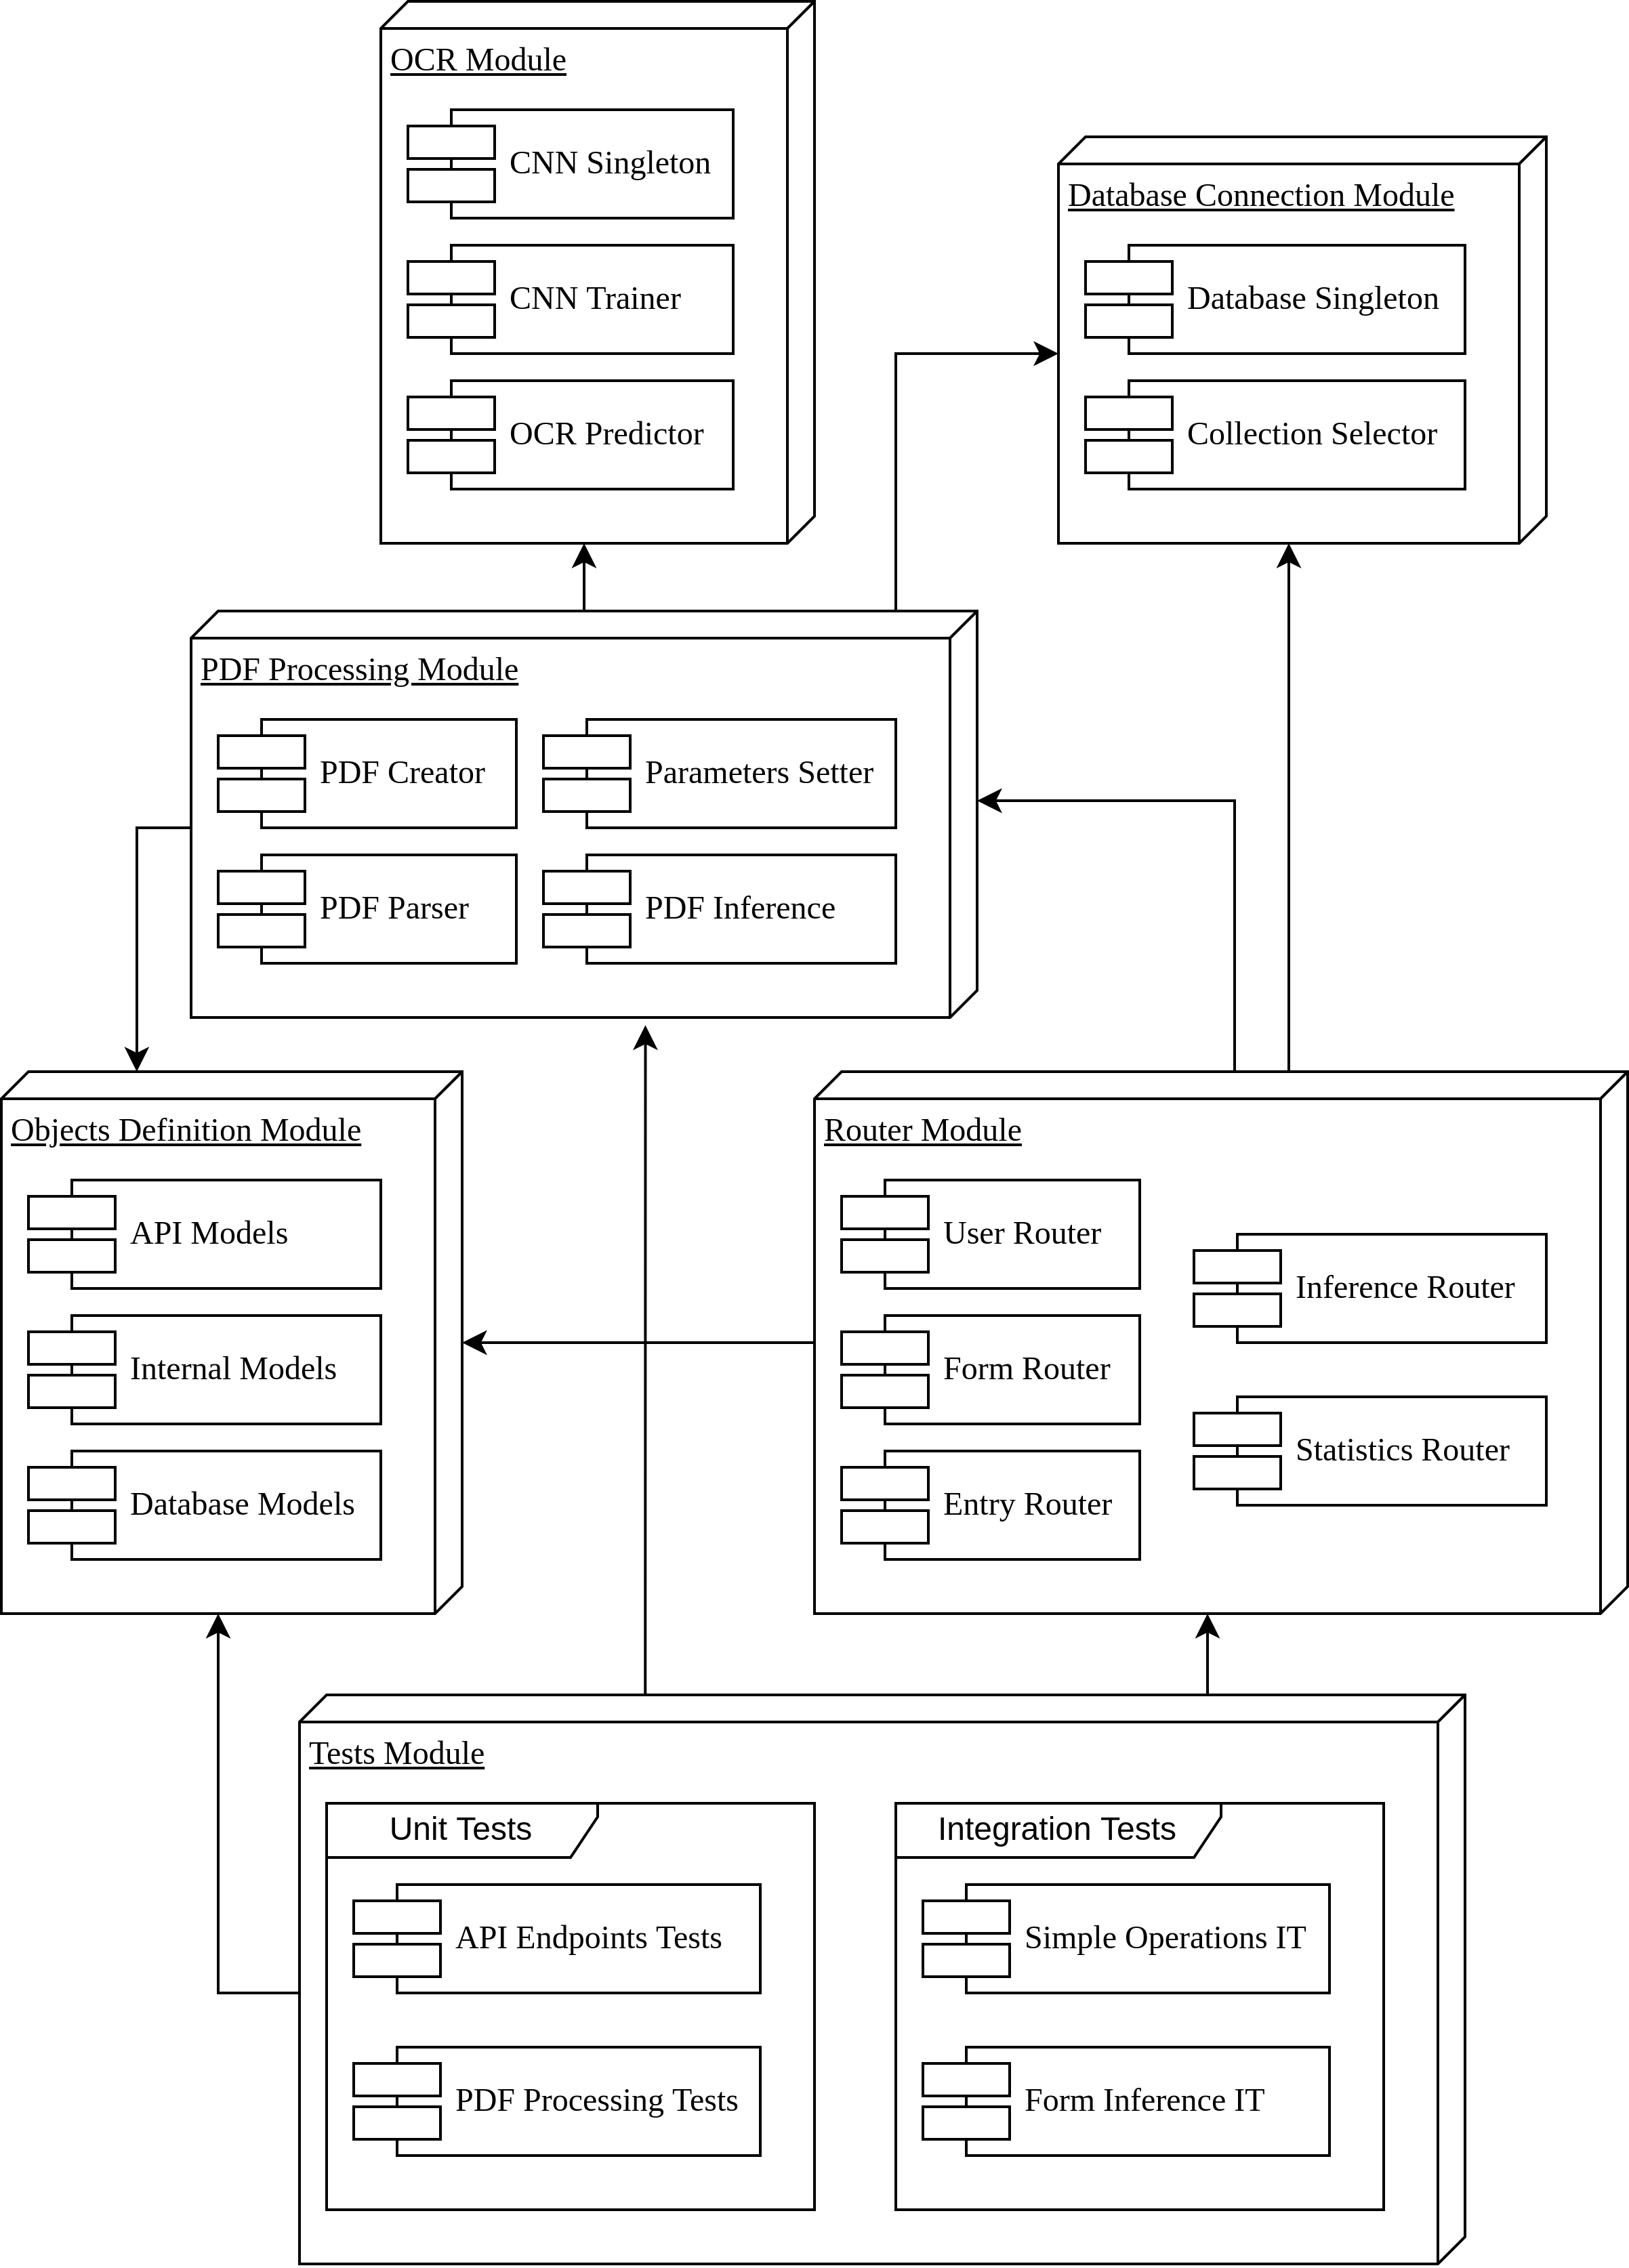
\includegraphics[width=37em]{images/diagrams/ProjectModulesDiagram.png}
	\caption{UML Diagram Of SmartForms's Backend Modules}
	\label{smart-forms-modules}
\end{figure}


% explic cum functioneaza aplicatia
\chapter{Detailed Overview of the API}

\section{What is an API, and why do we need one?}

The API -- or \textbf{A}pplication \textbf{P}rogramming \textbf{I}nterface is an interface acting like a bridge between applications, essentially allowing for an over-the-network communication between them.

The most common API implementations are made with the help of the \textit{HTTP} protocol, an application-layer protocol on top of the \textit{TCP/IP} stack. For showcasing the utility of using an API, we can make a simple request to get the current time:

\definecolor{bg}{rgb}{0.95,0.95,0.95}
\begin{minted}[bgcolor=bg]{Shell}
teom@lapttop ~> curl "http://worldtimeapi.org/api/timezone/Europe/Bucharest"\
                 | python -m json.tool
  % Total    % Received % Xferd  Average Speed   Time    Time     Time  Current
                                 Dload  Upload   Total   Spent    Left  Speed
100   395  100   395    0     0   1220      0 --:--:-- --:--:-- --:--:--  1222
{
    "abbreviation": "EEST",
    "client_ip": "5.12.1.116",
    "datetime": "2022-05-20T12:17:44.160367+03:00",
    "day_of_week": 5,
    "day_of_year": 140,
    "dst": true,
    "dst_from": "2022-03-27T01:00:00+00:00",
    "dst_offset": 3600,
    "dst_until": "2022-10-30T01:00:00+00:00",
    "raw_offset": 7200,
    "timezone": "Europe/Bucharest",
    "unixtime": 1653038264,
    "utc_datetime": "2022-05-20T09:17:44.160367+00:00",
    "utc_offset": "+03:00",
    "week_number": 20
}
\end{minted}

This shell script uses the \textit{curl} program, used for querying content over the network, which:
\begin{enumerate}
    \item Breaks down the \textit{URL} we requested (\code{http://worldtimeapi.org/api/timezone/Europe/Bucharest}) into two components:
    \begin{itemize}
        \item The domain -- \code{http://worldtimeapi.org}, which in turn is changed into an \textit{IP} address with the help of a \textit{DNS} server.
        \item The resource path (or route) -- \code{/api/timezone/Europe/Bucharest}, used by the API server to determine what information we want to receive.
    \end{itemize}
    \item Sends the request to the API server.
    \item Receives back a payload, which is piped into the \textit{Python} \textit{JSON} displaying tool to be easier to read.
\end{enumerate}

In the example above, the API function we called doesn't have any side-effects -- it doesn't change the internal state of the server. However, in most practical cases, the API exposes functions mutating the stored information.

\section{SmartForms \textit{API}}

The entire \textit{SmartForms} backend software is aimed at being able to respond to API calls.\\
In this section we will go over all of the available endpoints of the \textit{API}, presenting all of the user-facing functionalities of the application. They are divided into categories, each one determined by its path and served by a different router.

Note that we will only give a short description of the available endpoints (the \textit{HTTP Verb} and the path used). To see additional details such as parameters or security restrictions, please check the resources mentioned in the appendix.

\subsection{User Router}

This router exposes functionalities relating to the authentication, registration and deletion of accounts from the platform.

Its endpoints are:
\begin{itemize}
    \item \code{GET /api/user} -- shows a simple message telling the user if he/she is logged in, and promps it to sign in or sign out.
    \item \code{GET /api/user/login} and \code{GET /api/user/auth} -- both endpoints help the user to sign-in and sign-up.
    \item \code{GET /api/logout} -- signs out the user.
    \item \code{DELETE /api/delete-account} -- deletes the user's account, his/her forms and his/her entries.
\end{itemize}

\subsection{Form Router}

This router handles the \textit{PDF} form creation, modification, deletion, and retrieval. Its endpoints are:
\begin{itemize}
    \item \code{POST /api/form/preview} -- receives a description of a form (questions, title, author etc) and returns a preview of the final \textit{PDF} form. This is specially useful as users tend to try out multiple formats before settling for a form.
    \item \code{POST /api/form/create} -- similar to the \textit{preview} endpoint, but commits the created form to the database.
    \item \code{POST /api/form/list} -- returns a list of available forms, depending on filtering criteria.
    \item \code{GET /api/description/\{formId\}} -- returns the description of a given form.
    \item \code{GET /api/form/pdf/\{formId\}} -- returns the \textit{Base64} encoding of the \textit{PDF} representation of a given form.
    \item \code{DELETE /api/form/delete/\{formId\}} -- deletes the form and all of its associated answers.
    \item \code{PUT /api/form/online-access/\{formId\}} -- updates the visibility of the form (for instance if anyone can submit an answer to it online).
\end{itemize}

Note that it is \textbf{not} possible to change the actual content of a form. This is by design, as having multiple versions of the same form would be a hassle. The \textit{update} of a form is done on the client-side, by simply cloning the description of the initial form and creating a new one.

\subsection{Entry Router}

Similarly to the \textit{Form Router}, the \textit{Entry Router} contains API endpoints manipulating entries (or answers). Its endpoints are:
\begin{itemize}
    \item \code{POST /api/entry/create} -- adds a new answer to a given form.
    \item \code{DELETE /api/entry/delete/\{entryId\}} -- deletes the entry with the given Id.
    \item \code{PUT /api/entry/edit} -- deletes the entry with the given Id.
    \item \code{GET /api/entry/view-entry/\{entryId\}} -- returns the information provided in the given answer.
    \item \code{POST /api/entry/view-form-entries} -- returns a list of forms respecting a set of given criteria.
\end{itemize}

\subsection{Inference Router}

The single scope of the \textit{Inference Router} is to receive pictures of forms filled by hand, which are then parsed.

When the software is able to detect a form, it parses it and extracts the answer, which is then added to the database. The endpoint is \code{POST /api/inference/infer}.
\\ \\
Another functionality of the \textit{Inference Router} is to extract character data, in order to generate a character dataset:
\begin{enumerate}
    \item When an answer is uploaded, the \code{infer} endpoint saves for each character the corresponding sub-image containing its pixels.
    \item If the answer is later modified, then an annotated character datapoint is generated.
    \item The OCR neural network is trained on the generated dataset.
\end{enumerate}

In other words, if the inference failed, a character is wrongly identified. If someone updates the answer with the correct one, then the software finds the difference and generates a new labeled character image it can then use to fine-tune the OCR neural network.

\subsection{Statistics Router}

The \textit{Statistics Router} is aimed at providing additional information about \textit{SmartForms}.

Currently, the only available endpoint is \code{GET /api/statistics/global}, which returns information about the total number of forms and entries, but the router is implemented to simplify adding more advanced statistics in the future.

\section{Usage Scenario}

We will now present a simple usage scenario. We will communicate with the API using the \code{curl} command to better illustrate its functionality, but please note that in normal circumstances users only interact with the client, which performs the API calls in their behalf using the \code{fetch API}.

Let's create a new form, with the title "\textit{Sample Form}", and two questions, one asking for the user's gender and the other for his/her name:

\definecolor{bg}{rgb}{0.95,0.95,0.95}
\begin{minted}[bgcolor=bg]{Shell}
teo@fedora ~> curl -X 'POST' \
                    'http://smartforms.ml:5000/api/form/create' \
                    -H 'accept: application/json' \
                    -H 'Content-Type: application/json' \
                    -d '{
                "title": "Sample Form",
                "description": "Sample form to showcase the API.",
                "questions": [
                  {
                    "title": "Gender",
                    "description": "Boy or Girl",
                    "choices": [
                      "Boy",
                      "Girl"
                    ]
                  },
                  {
                    "title": "Name",
                    "description": "Enter your name, in uppercase.",
                    "maxAnswerLength": 36,
                    "allowedCharacters": "ABCDEFGHIJKLMNOPQRSTUVWXYZ "
                  }
                ],
                "canBeFilledOnline": true,
                "needsToBeSignedInToSubmit": true,
                "creationDate": "2022-05-24T07:29:36.216Z"
              }'
\end{minted}

We get back from the API the following \textit{JSON} object:
\definecolor{bg}{rgb}{0.95,0.95,0.95}
\begin{minted}[bgcolor=bg]{Shell}
{
    "formId": "af61ce94-db35-11ec-a6ed-dca6325bcf52",
    "formPdfBase64": "JVBERi0xLjMKMyAwIG9iago8PC9UeXBl...."
}
\end{minted}

We have now added the form to the database, and received back its Id and a \textit{Base64} encoding of its \textit{PDF} representation. Let's decode it.

We first have to manually copy the content of the \code{formPdfBase64} field, and we can then run:

\definecolor{bg}{rgb}{0.95,0.95,0.95}
\begin{minted}[bgcolor=bg]{Shell}
    teo@fedora ~> pbpaste | base64 -d > form.pdf
    teo@fedora ~> open form.pdf
\end{minted}

Please note that \code{pbpaste} is a non-standard utility outputing the content of the clipboard. The \code{open} command opened a \textit{PDF} viewer, with our form, as illustrated by Figure \ref{simple-form-preview}.

\begin{figure}[!h]
    \centering
    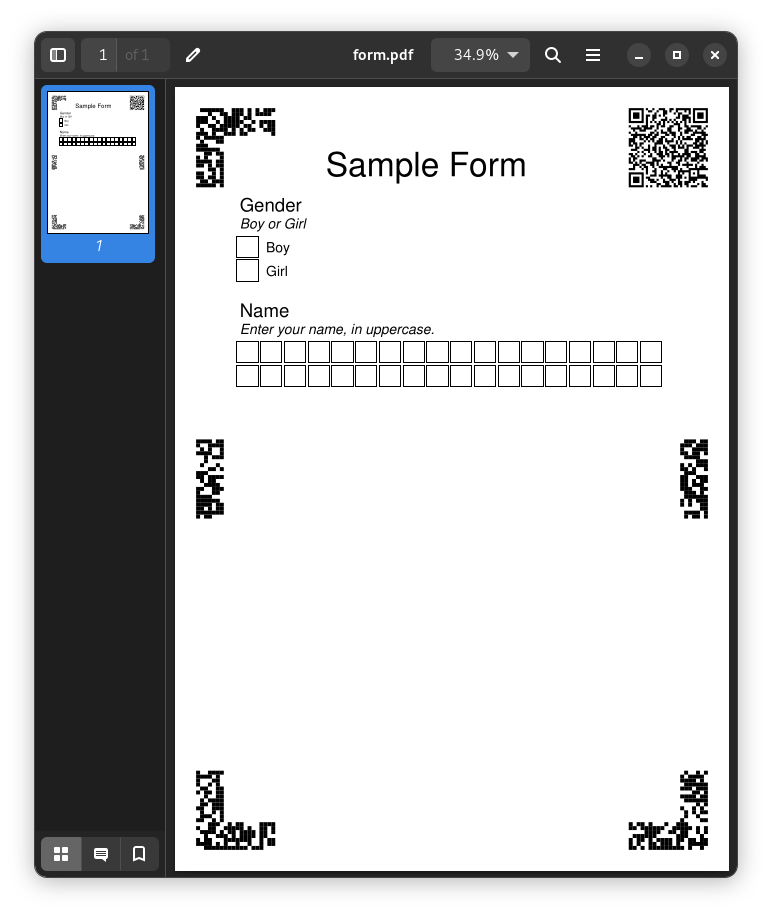
\includegraphics[width=20em]{images/screenshoots/sample_form.png}
    \caption{Sample form created with the SmartForms API}
    \label{simple-form-preview}
\end{figure}

The features of the \textit{PDF} document are:
\begin{itemize}
    \item The questions, where users are prompted to either write an '\code{X}', '\code{*}' or a similar symbol for multiple choice questions, and words for regular questions, one character per box.
    \item Lateral markers, forming a binary grid of small squares generated at random, which are added to maximize the number of features we can extract to match a scan / picture of the form with the original.
    \item The QR code (top right corner), playing a double role:
    \begin{itemize}
        \item Users can scan the form, which sends them to the webpage where they can fill the form online.
        \item The parsing software uses the QR code to extract the ID of the form, to retrieve the form's description from the database.
    \end{itemize}
\end{itemize}

We can now add an answer directly using the API (the \code{/api/entry/create} route):

\definecolor{bg}{rgb}{0.95,0.95,0.95}
\begin{minted}[bgcolor=bg]{Shell}
teo@fedora ~> curl -X 'POST' \
                    'http://smartforms.ml:5000/api/entry/create' \
                    -H 'accept: application/json' \
                    -H 'Content-Type: application/json' \
                    -d '{
                "answerId": "",
                "formId": "af61ce94-db35-11ec-a6ed-dca6325bcf52",
                "authorEmail": "",
                "answers": [
                  "X ",
                  "Theodor Moroianu"
                ]
              }'
# the command returns the following JSON:
{
    "entryId":"entry-04896360-db67-11ec-a6ed-dca6325bcf52"
}
\end{minted}

We can also print the form, and fill it by hand. We can then pass to the inference API the scan showed in Figure \ref{scan-of-filled-form}.

\begin{figure}[!h]
    \centering
    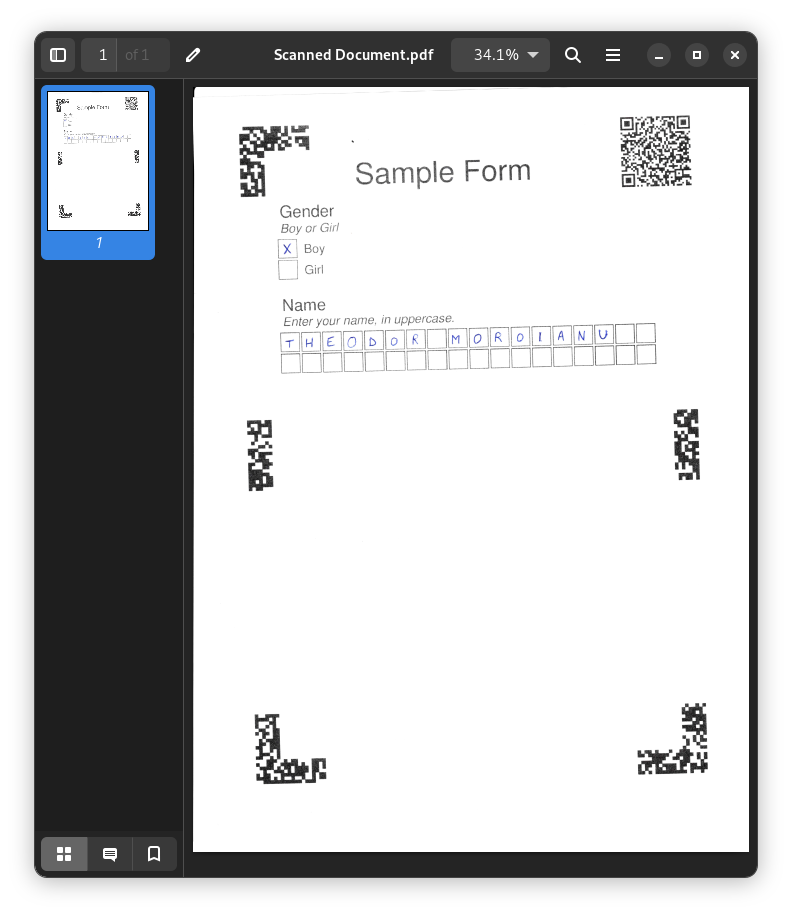
\includegraphics[width=30em]{images/screenshoots/sample_form_scan.png}
    \caption{Scan of a manually filled form}
    \label{scan-of-filled-form}
\end{figure}


We then get back the following data:

\definecolor{bg}{rgb}{0.95,0.95,0.95}
\begin{minted}[bgcolor=bg]{Shell}
{
  "entries": [
    {
      "answerId": "entry-b7ef7ca8-db69-11ec-a510-704d7ba4fc42",
      "formId": "af61ce94-db35-11ec-a6ed-dca6325bcf52",
      "authorEmail": "theodor.moroianu@gmail.com",
      "answers": [
        "X ",
        "THEODOR MOROIANU                    "
      ],
      "creationDate": "2022-05-24T16:59:24.561788"
    }
  ],
  "errors": []
}
\end{minted}

SmartForms is able to:
\begin{enumerate}
    \item Correctly detect, from the QR code, the form present in the scan.
    \item Extract each individual answer square.
    \item Run the squares through an OCR neural network, to predict the most plausible character.
    \item Add the answers to the database and return them to the users.
\end{enumerate}

It should be noted that the process is not flawless, and is discussed in more details in the Form Parsing section.
\\


We can now query the API to retrieve our two entries:

\definecolor{bg}{rgb}{0.95,0.95,0.95}
\begin{minted}[bgcolor=bg]{Shell}
teo@fedora ~> curl -X 'POST' \
                    'http://smartforms.ml:5000/api/entry/view-form-entries' \
                    -H 'accept: application/json' \
                    -H 'Content-Type: application/json' \
                    -d '{
                "formId": "af61ce94-db35-11ec-a6ed-dca6325bcf52",
                "offset": 0,
                "count": 2
              }' | python -m json.tool
  % Total    % Received % Xferd  Average Speed   Time    Time     Time  Current
                                 Dload  Upload   Total   Spent    Left  Speed
100   568  100   485  100    83   1473    252 --:--:-- --:--:-- --:--:--  1726
{
    "entries": [
        {
            "answerId": "entry-04896360-db67-11ec-a6ed-dca6325bcf52",
            "formId": "af61ce94-db35-11ec-a6ed-dca6325bcf52",
            "authorEmail": "theodor.moroianu@gmail.com",
            "answers": [
                "X ",
                "Theodor Moroianu"
            ],
            "creationDate": "2022-05-24T13:40:04.586000"
        },
        {
            "answerId": "entry-b7ef7ca8-db69-11ec-a510-704d7ba4fc42",
            "formId": "af61ce94-db35-11ec-a6ed-dca6325bcf52",
            "authorEmail": "theodor.moroianu@gmail.com",
            "answers": [
                "X ",
                "THEDDOR MOROIANU                    "
            ],
            "creationDate": "2022-05-24T16:59:24.561000"
        }
    ],
    "totalFormsCount": 2
}
\end{minted}

We can, in a similar fashion, edit / delete answers and forms.


% dau mai multe detalii despre cum 
% functioneaza baza de date mongodb
\chapter{Storage System}

\section{Choosing MongoDB}
We explored multiple database systems for our application. For choosing the most suited one, we made a list of requirements:

\begin{itemize}
    \item We need an easy to set-up, efficient system we can install on relatively small devices.
    \item We need a system well integrated within the \textit{Python} ecosystem.
    \item We need a system able to run both locally and in the cloud, to accommodate the different working scenarios of \textit{SmartForms}.
\end{itemize}

On the other hand, we do not need:
\begin{itemize}
    \item A system able to process massive amounts of data, as the database is mainly used for storing form descriptions and form answers.
    \item A system able to perform complex \code{joins} or similar operations typically done with the help of a \textit{DML} (Data Manipulation Language). 
\end{itemize}

The database system we decided to use within \textit{SmartForms} is \textit{MongoDB}, a document-based, No-SQL database storing data as \textit{JSON} objects.


\begin{figure}[!h]
    \centering
    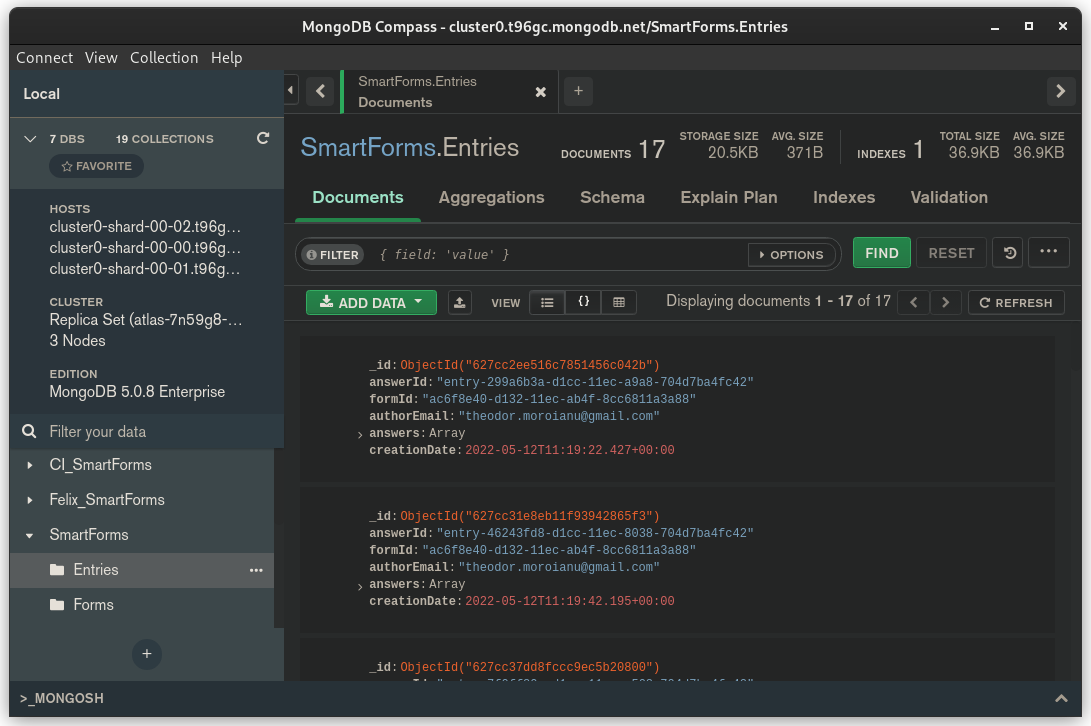
\includegraphics[width=35em]{images/screenshoots/mongo-compas.png}
    \caption{Compass -- the official MongoDB viewer}
    \label{fig:label}
\end{figure}

The connection to \textit{MongoDB} is done in the \code{database} module. The URI, username and password are specified with the help of the \code{.env} secrets file, which in the current configuration connects \textit{SmartForms} to a database stored on the cloud:

\definecolor{bg}{rgb}{0.95,0.95,0.95}
\begin{minted}[bgcolor=bg]{Shell}
# Connect to Mongo Cloud
MONGO_USER='smart-forms-user'
MONGO_PASSWORD='*********'
MONGO_CLUSTER='cluster0.t96gc.mongodb.net'
MONGO_DB_NAME='SmartForms'
\end{minted}

\section{Information Stored in MongoDB}

MongoDB databases, contain multiple collections storing entries, similar to SQL databases containing tables storing rows.

We set-up multiple databases:
\begin{itemize}
    \item A database used for production.
    \item Another database used for the \textit{CI/CD} pipelines.
    \item Databases used for local development and testing without disturbing the other environments. 
\end{itemize}

Databases store the information used by \textit{SmartForms}. As forms and answers requested by the users are unpredictable, and \textit{SmartForms} is built to be able to run on relatively low-end devices, locally caching data for lower latency didn't make sense. As such, any CRUD (Create, Read, Update or Delete) operations performed on forms, answers or users are directly committed to the database.


\begin{figure}[!h]
    \centering
    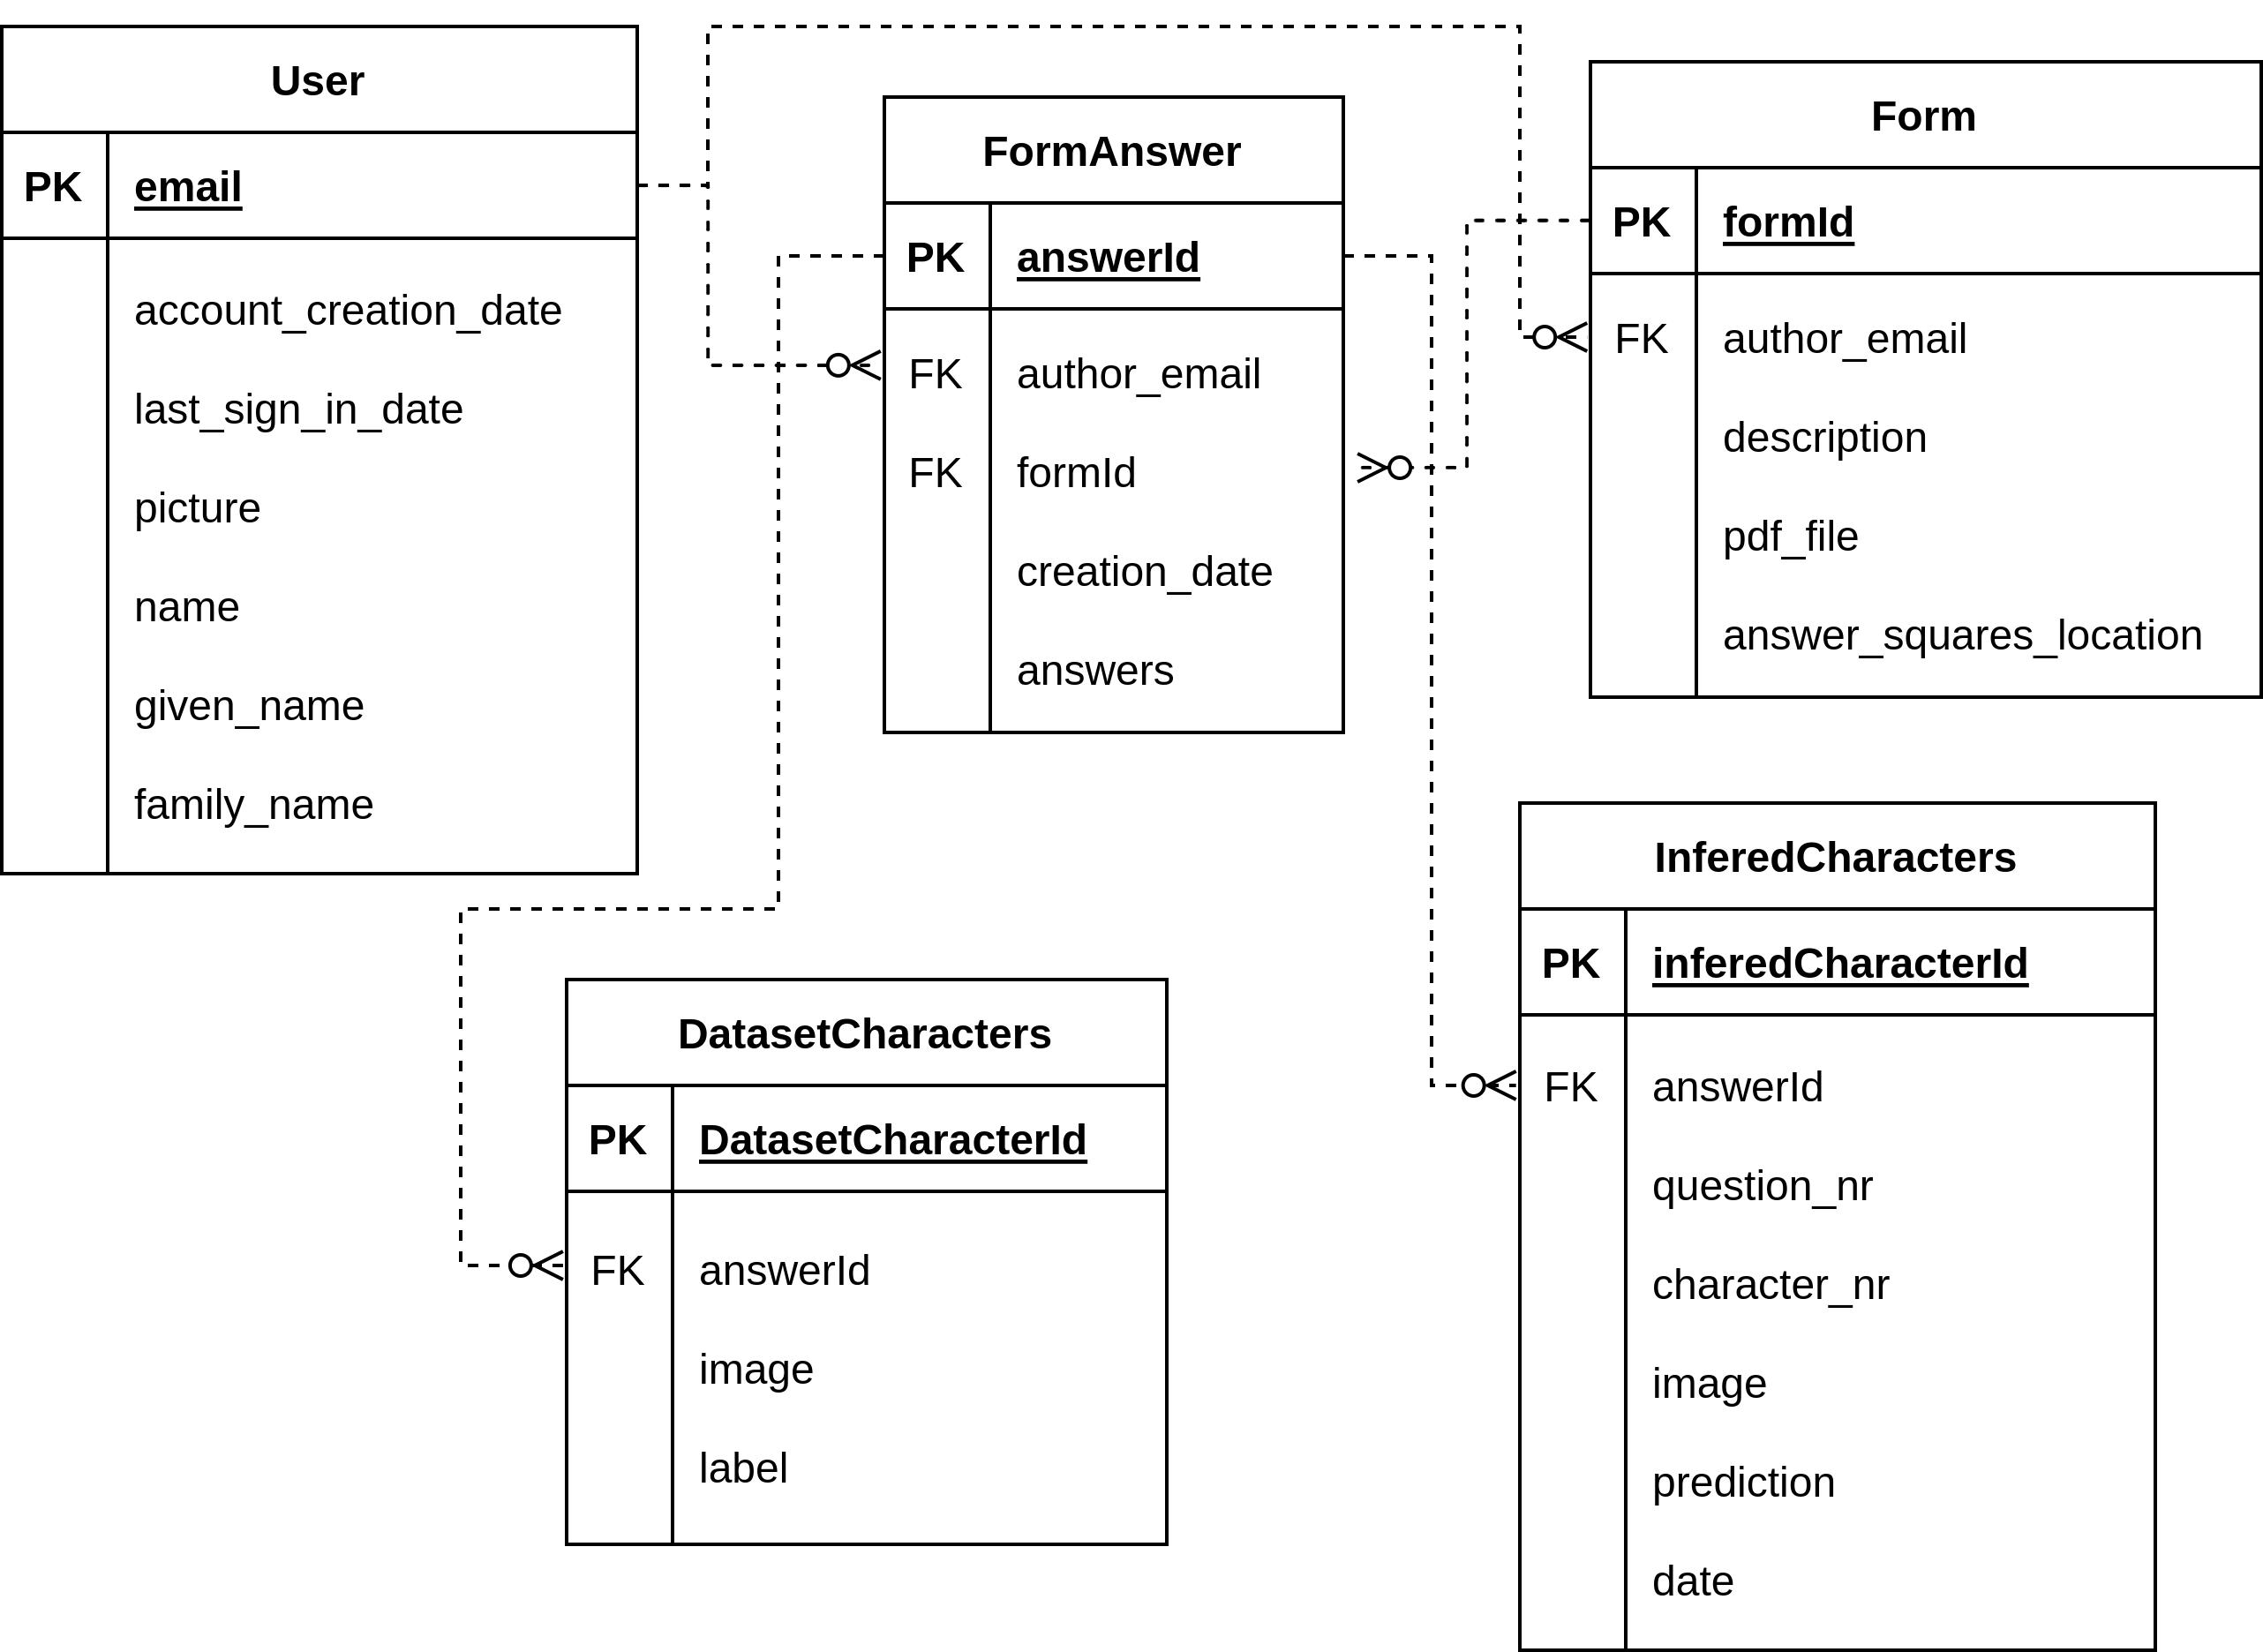
\includegraphics[width=35em]{images/diagrams/ER_diagram.png}
    \caption{Diagram of the MongoDB Database}
    \label{fig:label}
\end{figure}


The database stores:
\begin{itemize}
    \item The registered users. The information saved is the name, email, date of registration and last sign-in, and an URL to a profile picture if available. To be compliant with data-protection laws like the GDPR, we only use the personal data for authentication purposes, and delete all of an user's records when he/she deletes his/her account.
    \item The created forms -- for which we store the description, owner, creation date and the internal representation of the corresponding PDF document.
    \item The answers, both added directly with the API or uploaded as a scan or a picture.
    \item Images of the squares extracted from pictures and scans.
    \item A dataset of labeled characters which can be used for improving the OCR neural network.
\end{itemize}


The last two collection -- namely the \code{DatasetCharacters} and the \code{InferedCharacters} are used for automatically labeling characters, thus generating a dataset we can then use for fine-tuning the OCR neural network. A more detailed explanation of the process is done in the \textit{Form Parsing} section.


% Arat cum generez pdf-ul, si cum
% salvez un pdf generat.
\chapter{Pdf Forms Creation}

\section{Objective and Constraints}

Forms are not internally stored as \textit{PDF} documents. Users do not actually need to use \textit{PDF} documents at all, as one can create, share, and fill forms from the application itself. However, being able to have a printed copy of the form can be useful.

The primary objective when generating a \textit{PDF} form is getting a concise, easy to understand and professional looking document, which can then be efficiently parsed and digitized.

The main contraints and details we have to consider are:
\begin{itemize}
    \item While in most usecases users want to print their forms on \code{A4} paper, we should also make forms printable on smaller or larger paper.
    \item We want to allow both scans and pictures, made by a wide range of devices, in which brightness, color saturation and contrast differ.
    \item Modern smartphone cameras, because of the shrinkage of the size of their optical instruments, add slight distortions to the pictures (lines become curves). As each camera is different, fixing the distortions ourselves is not feasable.
    \item Even though most printers advertise the ability to print edge-to-edge, most modern printers are not able to print anything too close to the edges of the paper.
    \item As most office printers only print in black and white for efficiency reasons, we should not include color in our documents.
    \item People have extremely diverse styles of handwriting, which makes parsing cursive text with high accuracy difficult, even with modern technology.
    \item Forms can have varying lengths, from a simple question to multiple pages.
\end{itemize}

\section{Layout of a Pdf Form}

To not violate any of the constraints mentioned above, we embedd multiple components in the documents.

\subsection{Questions}

Questions are the most obvious element of the forms. They are made out of a question title -- or simply speaking the question, a question subtitle (or explanation) which is optional, and input zones depending on the type of question.

\begin{figure}[!h]
    \centering
    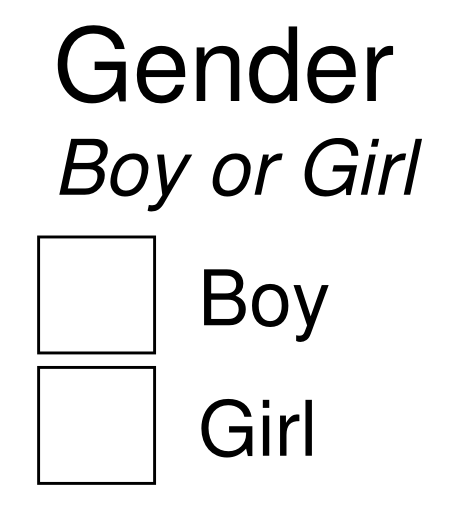
\includegraphics[width=8em]{images/screenshoots/sample-multiple-choice-question.png}
    \caption{Sample multiple-choice question}
    \label{multiple-choice-question}
\end{figure}

If the question is a multiple choice question as in Figure \ref{multiple-choice-question}, where the user has to select a subset of the given possibilities (e.g. "Boy" or "Girl"), each option is printed on a different line, with a square the user can tick to select the question.


\begin{figure}[!h]
    \centering
    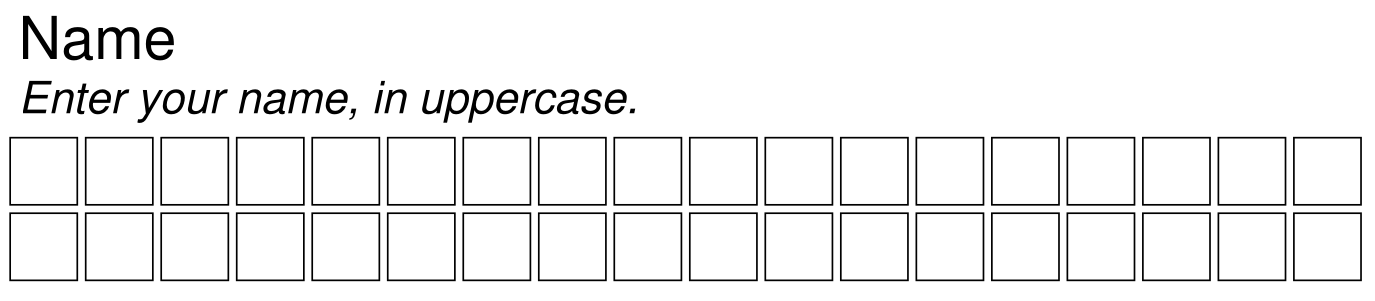
\includegraphics[width=40em]{images/screenshoots/sample-text-question.png}
    \caption{Sample text question}
    \label{text-question}
\end{figure}

If the question is a text question as in Figure \ref{text-question}, then a user-specified number of squares are printed. People filling the form can then write one letter per square.

The main advantages of this approach are:
\begin{itemize}
    \item Multiple-choice and text questions can be processed similarly, as we simply want to check if boxes from the multiple choice questions contain an '\code{X}', '\code{V}', '\code{*}', or a similar marker.
    \item This format is writing-style agnostic, as users are forced to write each letter to a specific location in a specific format.
    \item The forms are easy to understand and fill-in.
\end{itemize}

Note that the exact location of each square is saved in the database, to allow later pinpointing of the exact pixels of each character.

\subsection{Markers}

Lateral matching helpers, or markers, are irregular patterns we print on the corners.

\begin{figure}[!h]
    \centering
    
\includegraphics[width=10em]{images/screenshoots/top-left-marker.png}
    \caption{Top left marker}
    \label{fig:label2}
\end{figure}

Similar shapes are often printed on objects that robots or software agents need to be able to identify, due to their vast number of descriptors. \textit{SmartForms} uses a \textit{ORB} feature extractor\cite{rublee2011orb}, which relies on intensity differences between adjacent pixels.

With the help of the \textit{ORB} feature extractor, we can then match extracted features of the blank Pdf document with a picture or scan, to get an accurate rectangular representation of the scanned image.

\subsection{QR Code}

QR codes (shorthand for Quick Response codes) are visual machine barcodes. QR codes are machine-readable, use a powerful correction algorithm\cite{wicker1999reed} which makes them readable even when damaged, and can store arbitrary data, from Wi-Fi details to binary data or simple text.

\begin{figure}[!h]
    \centering
    
\includegraphics[width=13em]{images/screenshoots/sample-qr-code.png}
    \caption{QR code with content "\textit{https://smartforms.ml/view-form/af61...}"}
    \label{qr-code-image}
\end{figure}

We use QR codes for multiple reasons:
\begin{itemize}
    \item Due to their apparent randomness, they also help the feature extraction of the matching process.
    \item They offer an easy-to-follow link to the \textit{SmartForms} website, which users can open to fill the form online.
    \item It allows the matching software to extract the form ID, to figure out which form is being parsed.
\end{itemize}

\subsection{Preview Notice}

Users tend to commit their work more often than is strictly required: people writing documents save them every few minutes, developers writing code compile it to check for mistakes, and, to no surprise, people generating forms tend to preview intermediate results.

As such, adding each intermediate result to the database doesn't make much sense. On the other hand, users have to easily see if a form is valid or not. This is why, on forms which are only made for preview, we print an additional "\textit{PREVIEW}" banner.


\begin{figure}[!h]
    \centering
    \fbox{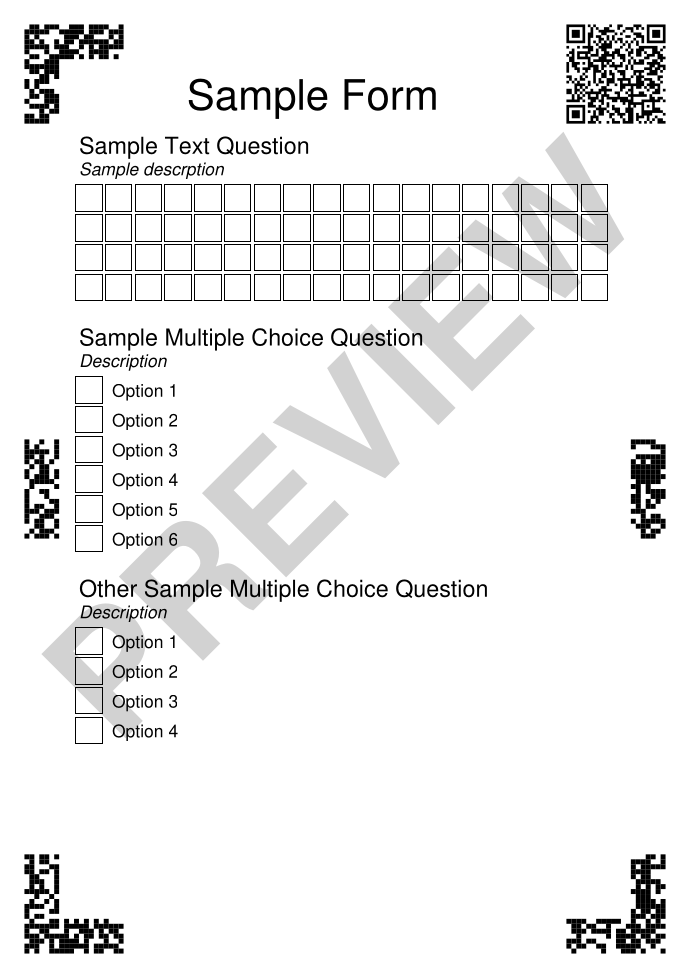
\includegraphics[width=30em]{images/screenshoots/sample-preview-form.png}}
    \caption{Form with "\textit{PREVIEW}" banner.}
    \label{fig:label3}
\end{figure}

\subsection{Multi-page Support}

If the form has many questions, then the \textit{PDF} document might spread among multiple pages. In such situations, each page gets a unique ID encoded within the QR code, to allow the parsing pipeline to order them accordingly.

The lateral markers and the optional preview notice are present on all the pages.



% Arat cum fac matchingul si ocr-ul.
% tot aici vorbesc despre CNN
\chapter{Form Parsing}

When a user has a list of handfilled documents he/she wishes to digitize, they just have to upload the files to \textit{SmartForms API} and let it parse the documents automatically.

\section{How Data is Loaded}

The API relies on the \code{multipart/form-data}\cite{masinter1998rfc2388} format to receive reliably larger files than what is usually permitted over the \textit{HTTP} protocol.

To facilitate the uploading of filled forms, we accept:
\begin{itemize}
    \item A list of images, in any of the standard image formats (\code{.jpeg}, \code{.png}, \code{.webp} etc).
    \item A list of \textit{PDF} documents.
    \item A \textit{ZIP} archive, the content of which is processed recursively.
\end{itemize}

Due to the high flexibility and permissive formats supported by \textit{SmartForms}, virtually any structured folder of forms can be zipped, uploaded and parsed.

Once the backend receives the files, it automatically deflates all \textit{ZIP} files, and:
\begin{enumerate}
    \item Considers each \textit{PDF} as a folder, whose content are the pages of the document (each page is considered as a single picture).
    \item Splits all the images into groups, according to their containing folder.
    \item Parses each group as a single form.
\end{enumerate}

\section{Finding the Template}

Given a set of images (obtained directly from the user, from a \textit{ZIP} file or extracted from a page of a \textit{PDF} document), the backend has to figure out which form is being parsed.

To do this quickly and reliably, we look for the QR code inserted on each document. Finding the QR code is itself a challenge, as most libraries used for scanning QR codes (like the ones used on mobile phones) expect a close-up picture of the code. However, because we can't know the orientation, size or location of the form in the received picture, we can't reliably determine the exact location of the QR code.

For solving this issue, we use \code{Zbar}, an open-source bar reading library written in \textit{C}. While the application isn't written in \textit{Python} for compatibility and performance reasons, the \code{pyzbar} package provides \textit{Python} bindings we can use.

\textit{Zbar} is highly optimized for real-time barcodes and QR codes scanning, and can be also used from a terminal. By passing it the form we created above we get:


\definecolor{bg}{rgb}{0.95,0.95,0.95}
\begin{minted}[bgcolor=bg]{Shell}
teo@fedora ~> zbarimg Scanned\ Document.pdf 
QR-Code:
https://smartforms.ml/view-form/af61ce94-db35-11ec-a6ed-dca6325bcf52

scanned 1 barcode symbols from 1 images in 0.02 seconds
\end{minted}

Please note that the text extracted by \textit{Zbar} is not the actual ID of the form, but rather an URL to the \textit{SmartForms} website, where, depending on permissions, users may fill the form online. To extract the real ID, we simply have to remove the "\textit{https://smartforms.ml/view-form/}" prefix. \textit{Pyzbar} operates in a similar way as its command-line counterpart, but can be called from within \textit{Python} code.

With the form ID, we can query the \textit{MongoDB} database to extract all the required details about the form.

\section{Applying Graysclale and Binary Threshold}

\begin{figure}[!h]
\hfill
\subfigure[Original]{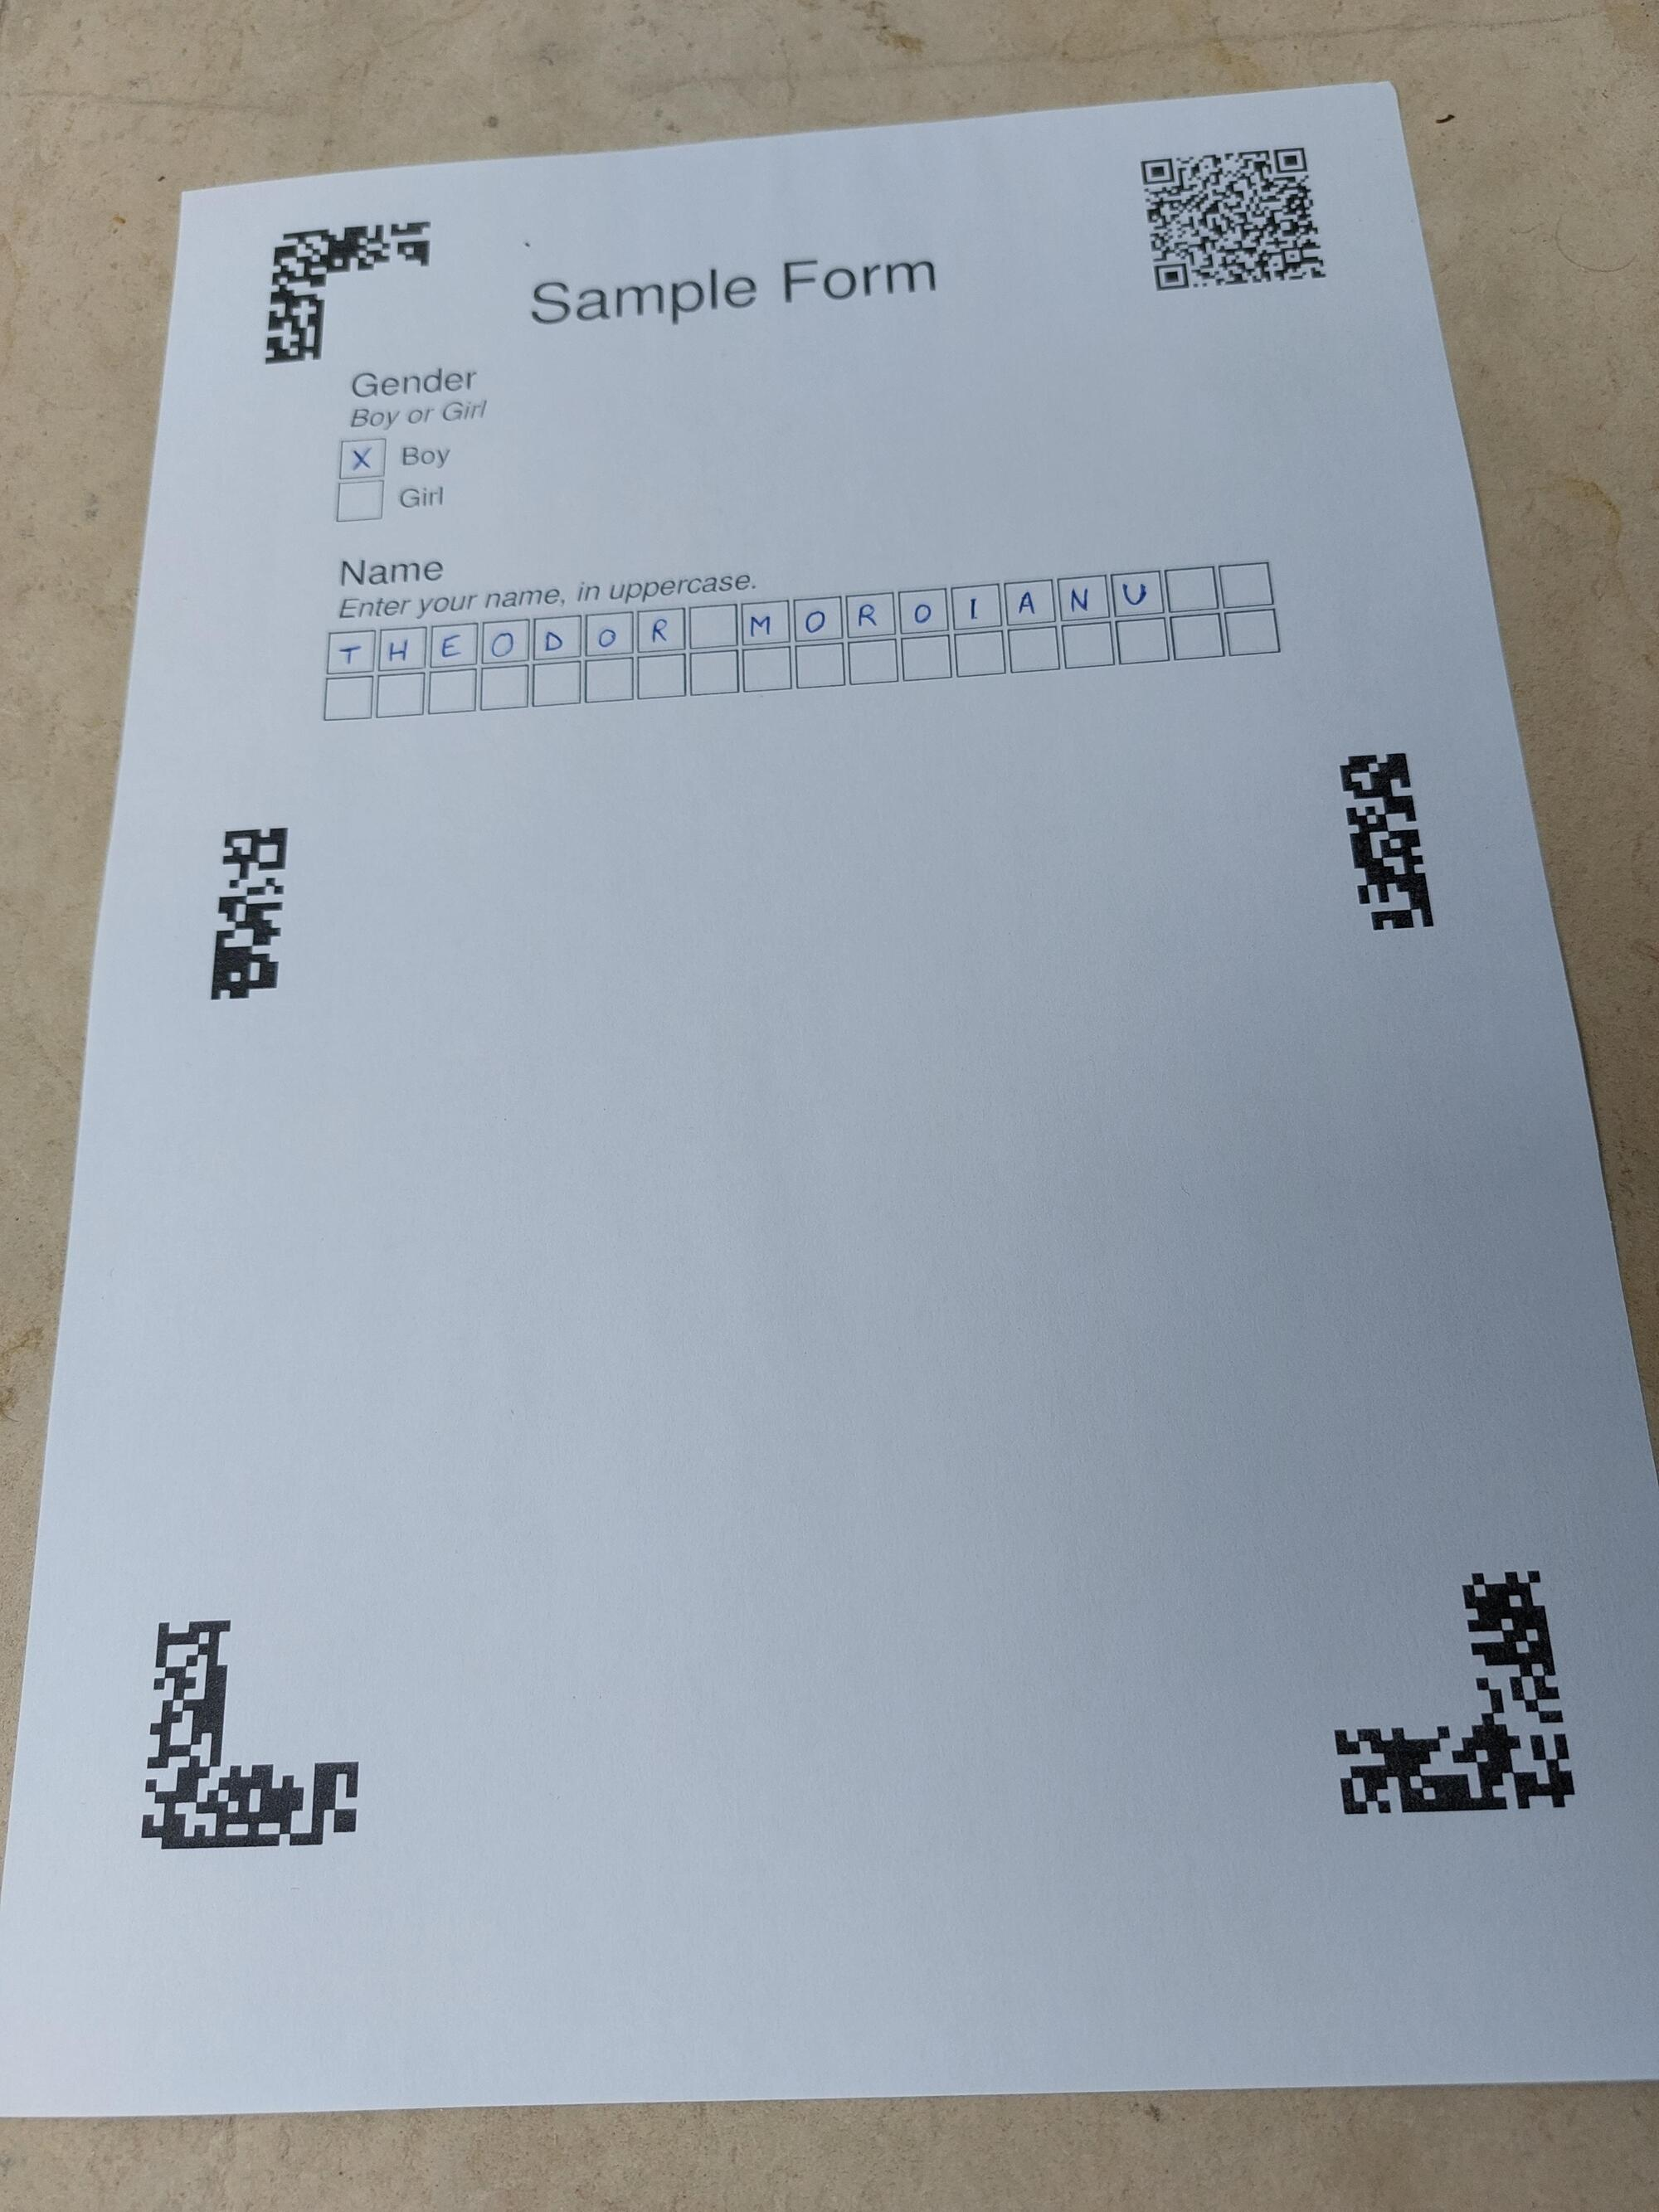
\includegraphics[width=6cm]{images/graphs/original_image_fixed.jpg}}
% \hfill
\subfigure[Processed]{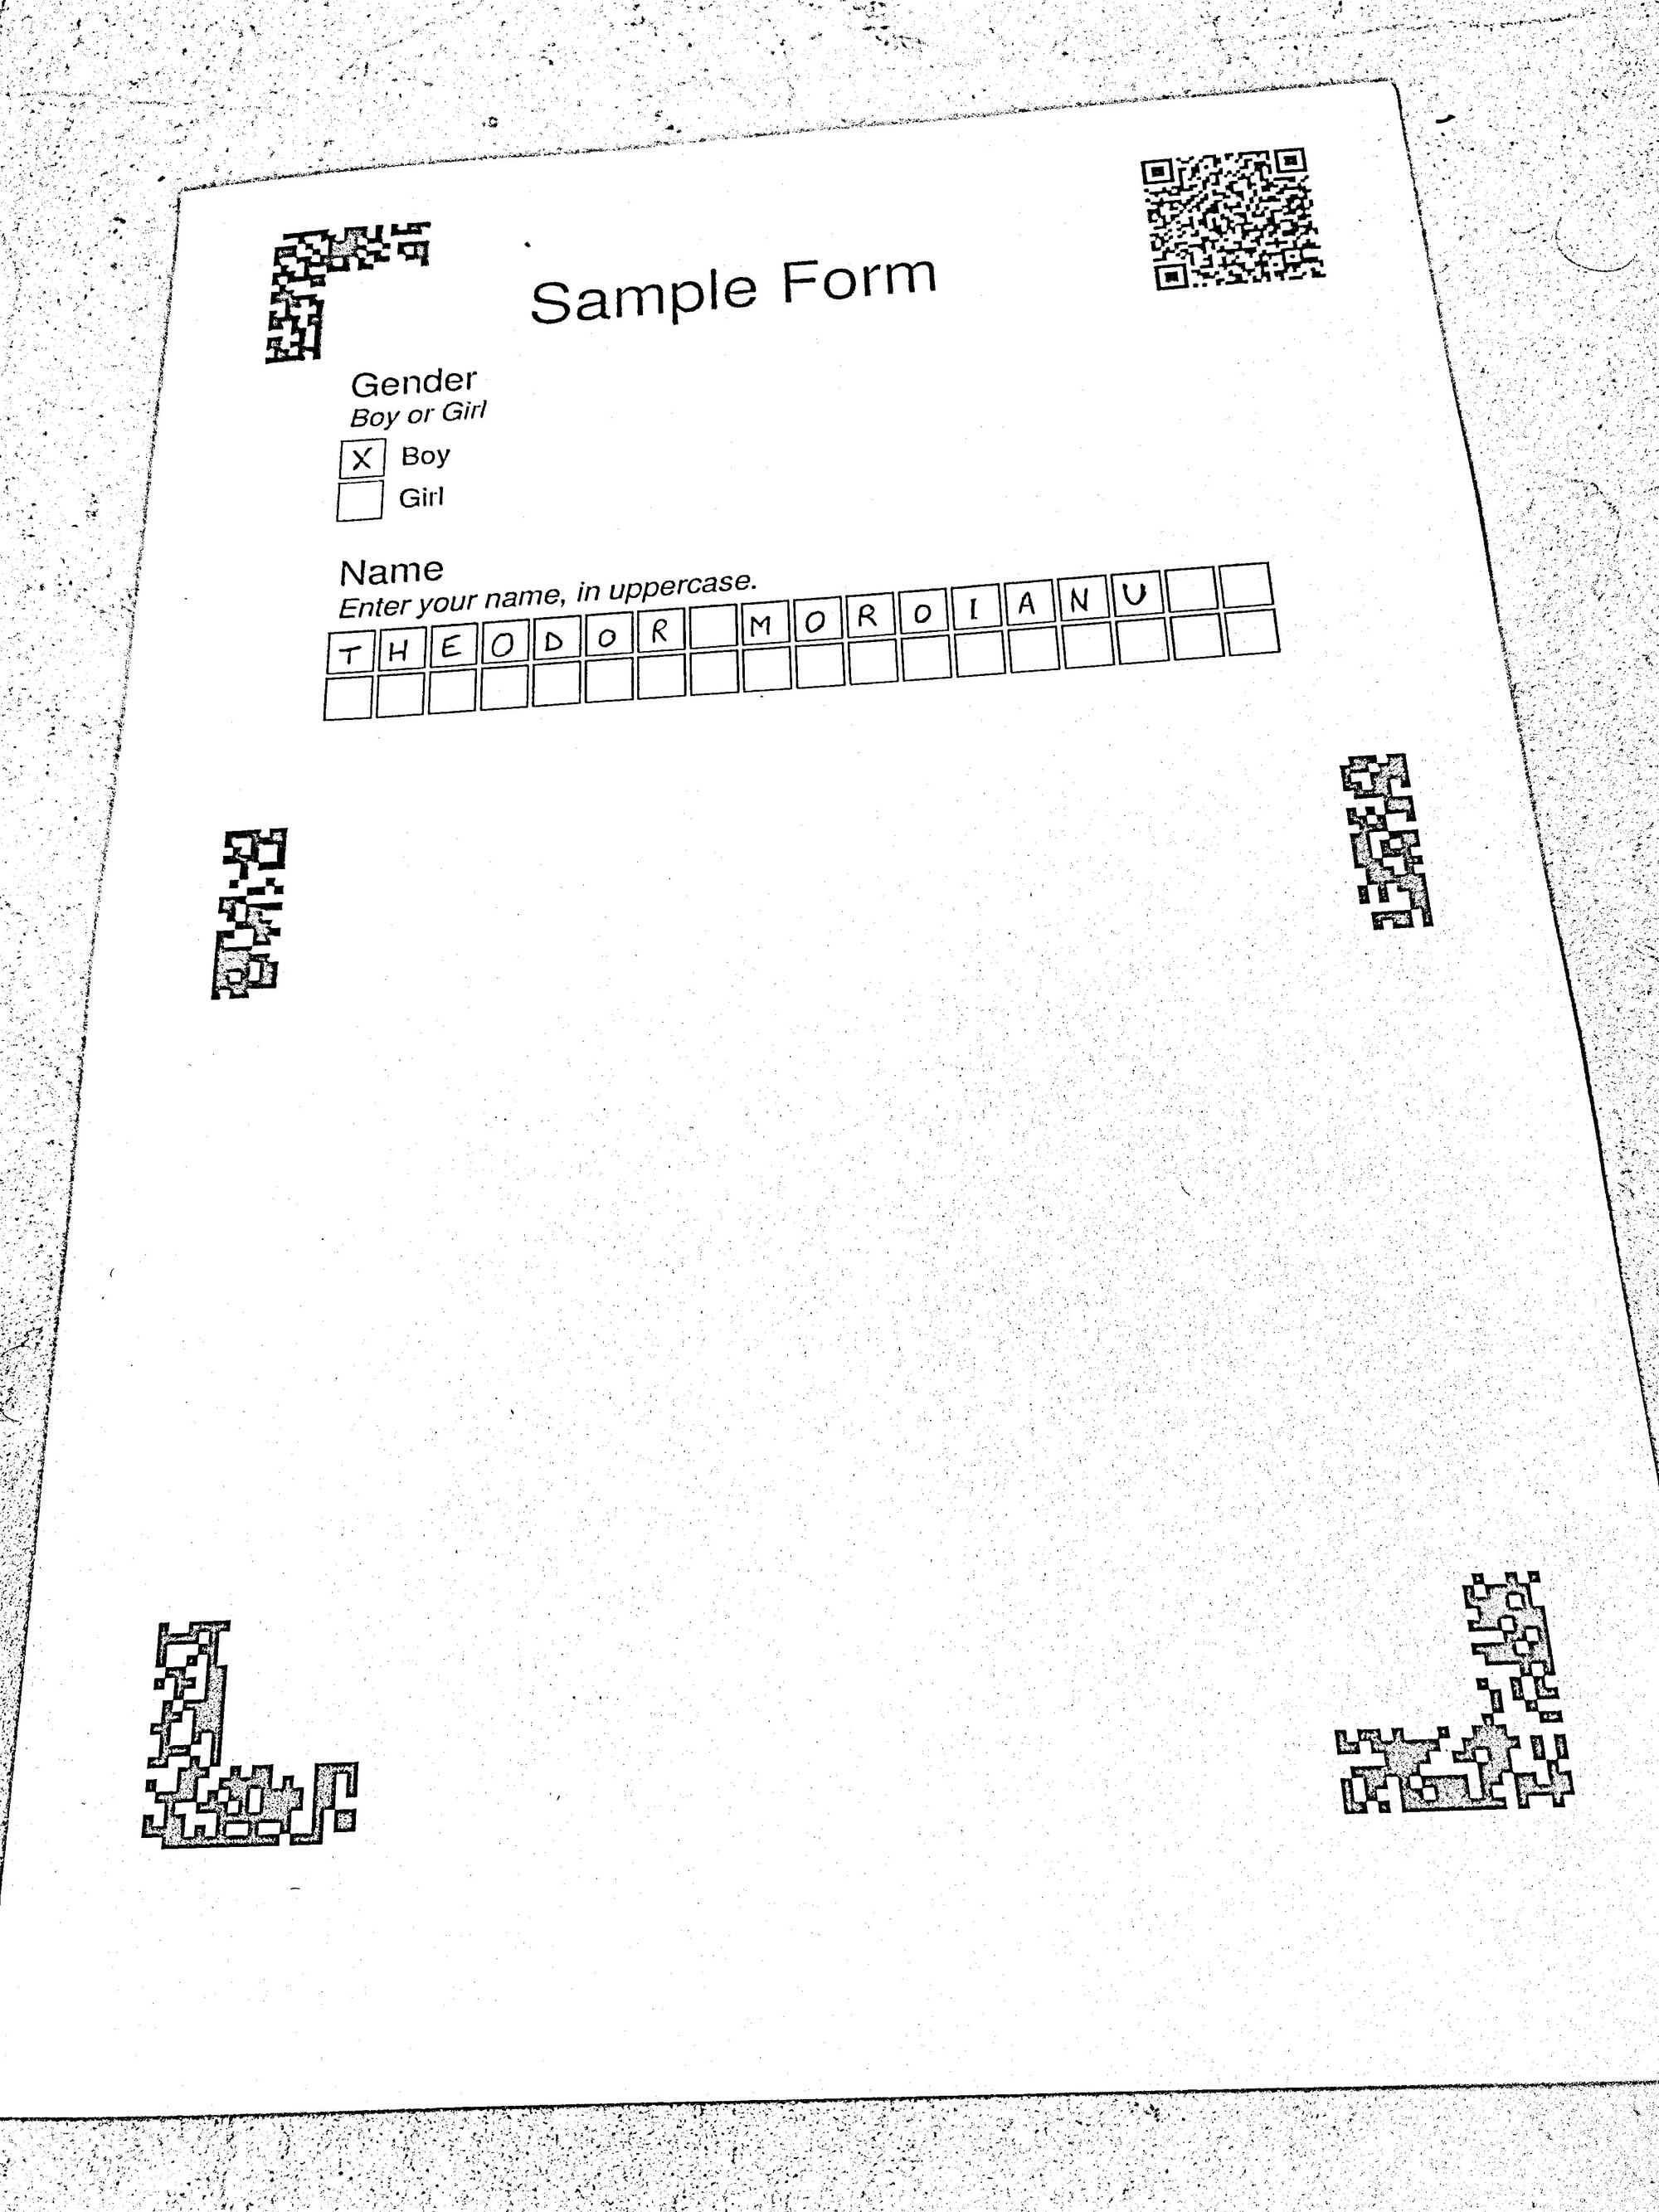
\includegraphics[width=6cm]{images/graphs/parser_processed_image_fixed.jpg}}
\hfill
\caption{Picture converted to binary}
\label{original-vs-processed-image}
\end{figure}

Most image processing algorithms rely on grayscale or binary images. As such, we first have to convert our colored image to grayscale, and then apply a binary threshold.

To convert an image to grayscale, we can independently transform each pixel from a \code{RGB} value to a single channel. \textit{OpenCV}, the machine vision framework we are using, converts an image to grayscale using the following formula\cite{opencv-color-convention}:

$$Y = 0.299*R+0.587*G+0.114*B$$

Our first step is converting a picture or scan of our form into grayscale. Figure \ref{original-vs-processed-image} (a) shows what such a picture might look like. However, even with the image in grayscale we cannot simply apply a standard binary threshold, due to possible differences in brightness.

 \begin{figure}[!h]
  \centering
  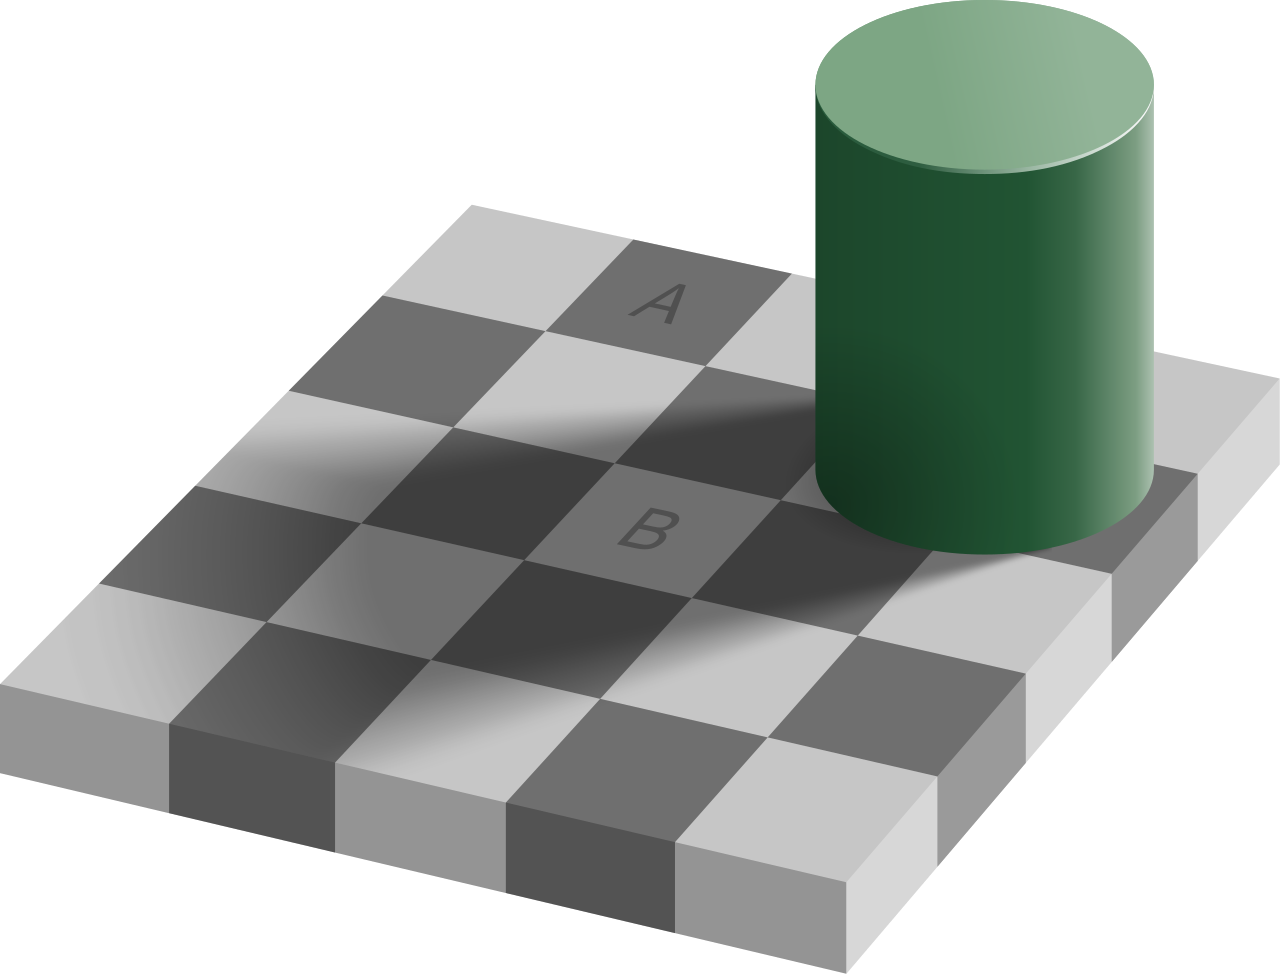
\includegraphics[width=20em]{images/other/Checker_shadow_illusion.svg.png}
  \caption{Checker Shadow Illusion\cite{checker-illusion}}
  \label{checker-illusion}
\end{figure}

As ilustrated in Figure \ref{checker-illusion}, where squares marked with \textbf{A} and \textbf{B} seem different even though the color is the same, separating dark and light regions is not a trivial task, if we want to take into account lighing and brightness. Similarly, applying a binary threshold considering pixel intensities larger than a fixed $K$ black and intensities smaller than $K$ white will lead to misclassified pixels, where darker empty regions of the form might be classified as black, and similarly lighter text or graphics of the form might get classified as white.

To convert our grayscale image to binary, we use an adaptive thresholding technique\cite{opencv-image-threshold}, which for each pixels determines, based on a small region around it, if it should be black or white. Applying such an algorithm over our grayscale image gives us an image similar to Figure \ref{original-vs-processed-image} (b).


%Ca in figura \ref{etichetaTT}

\section{Changing Image Perspective}

% \begin{figure}[!h]%
%     \centering
%     \subfloat[\centering label 1]{{
%     \rotatebox[origin=c]{90}{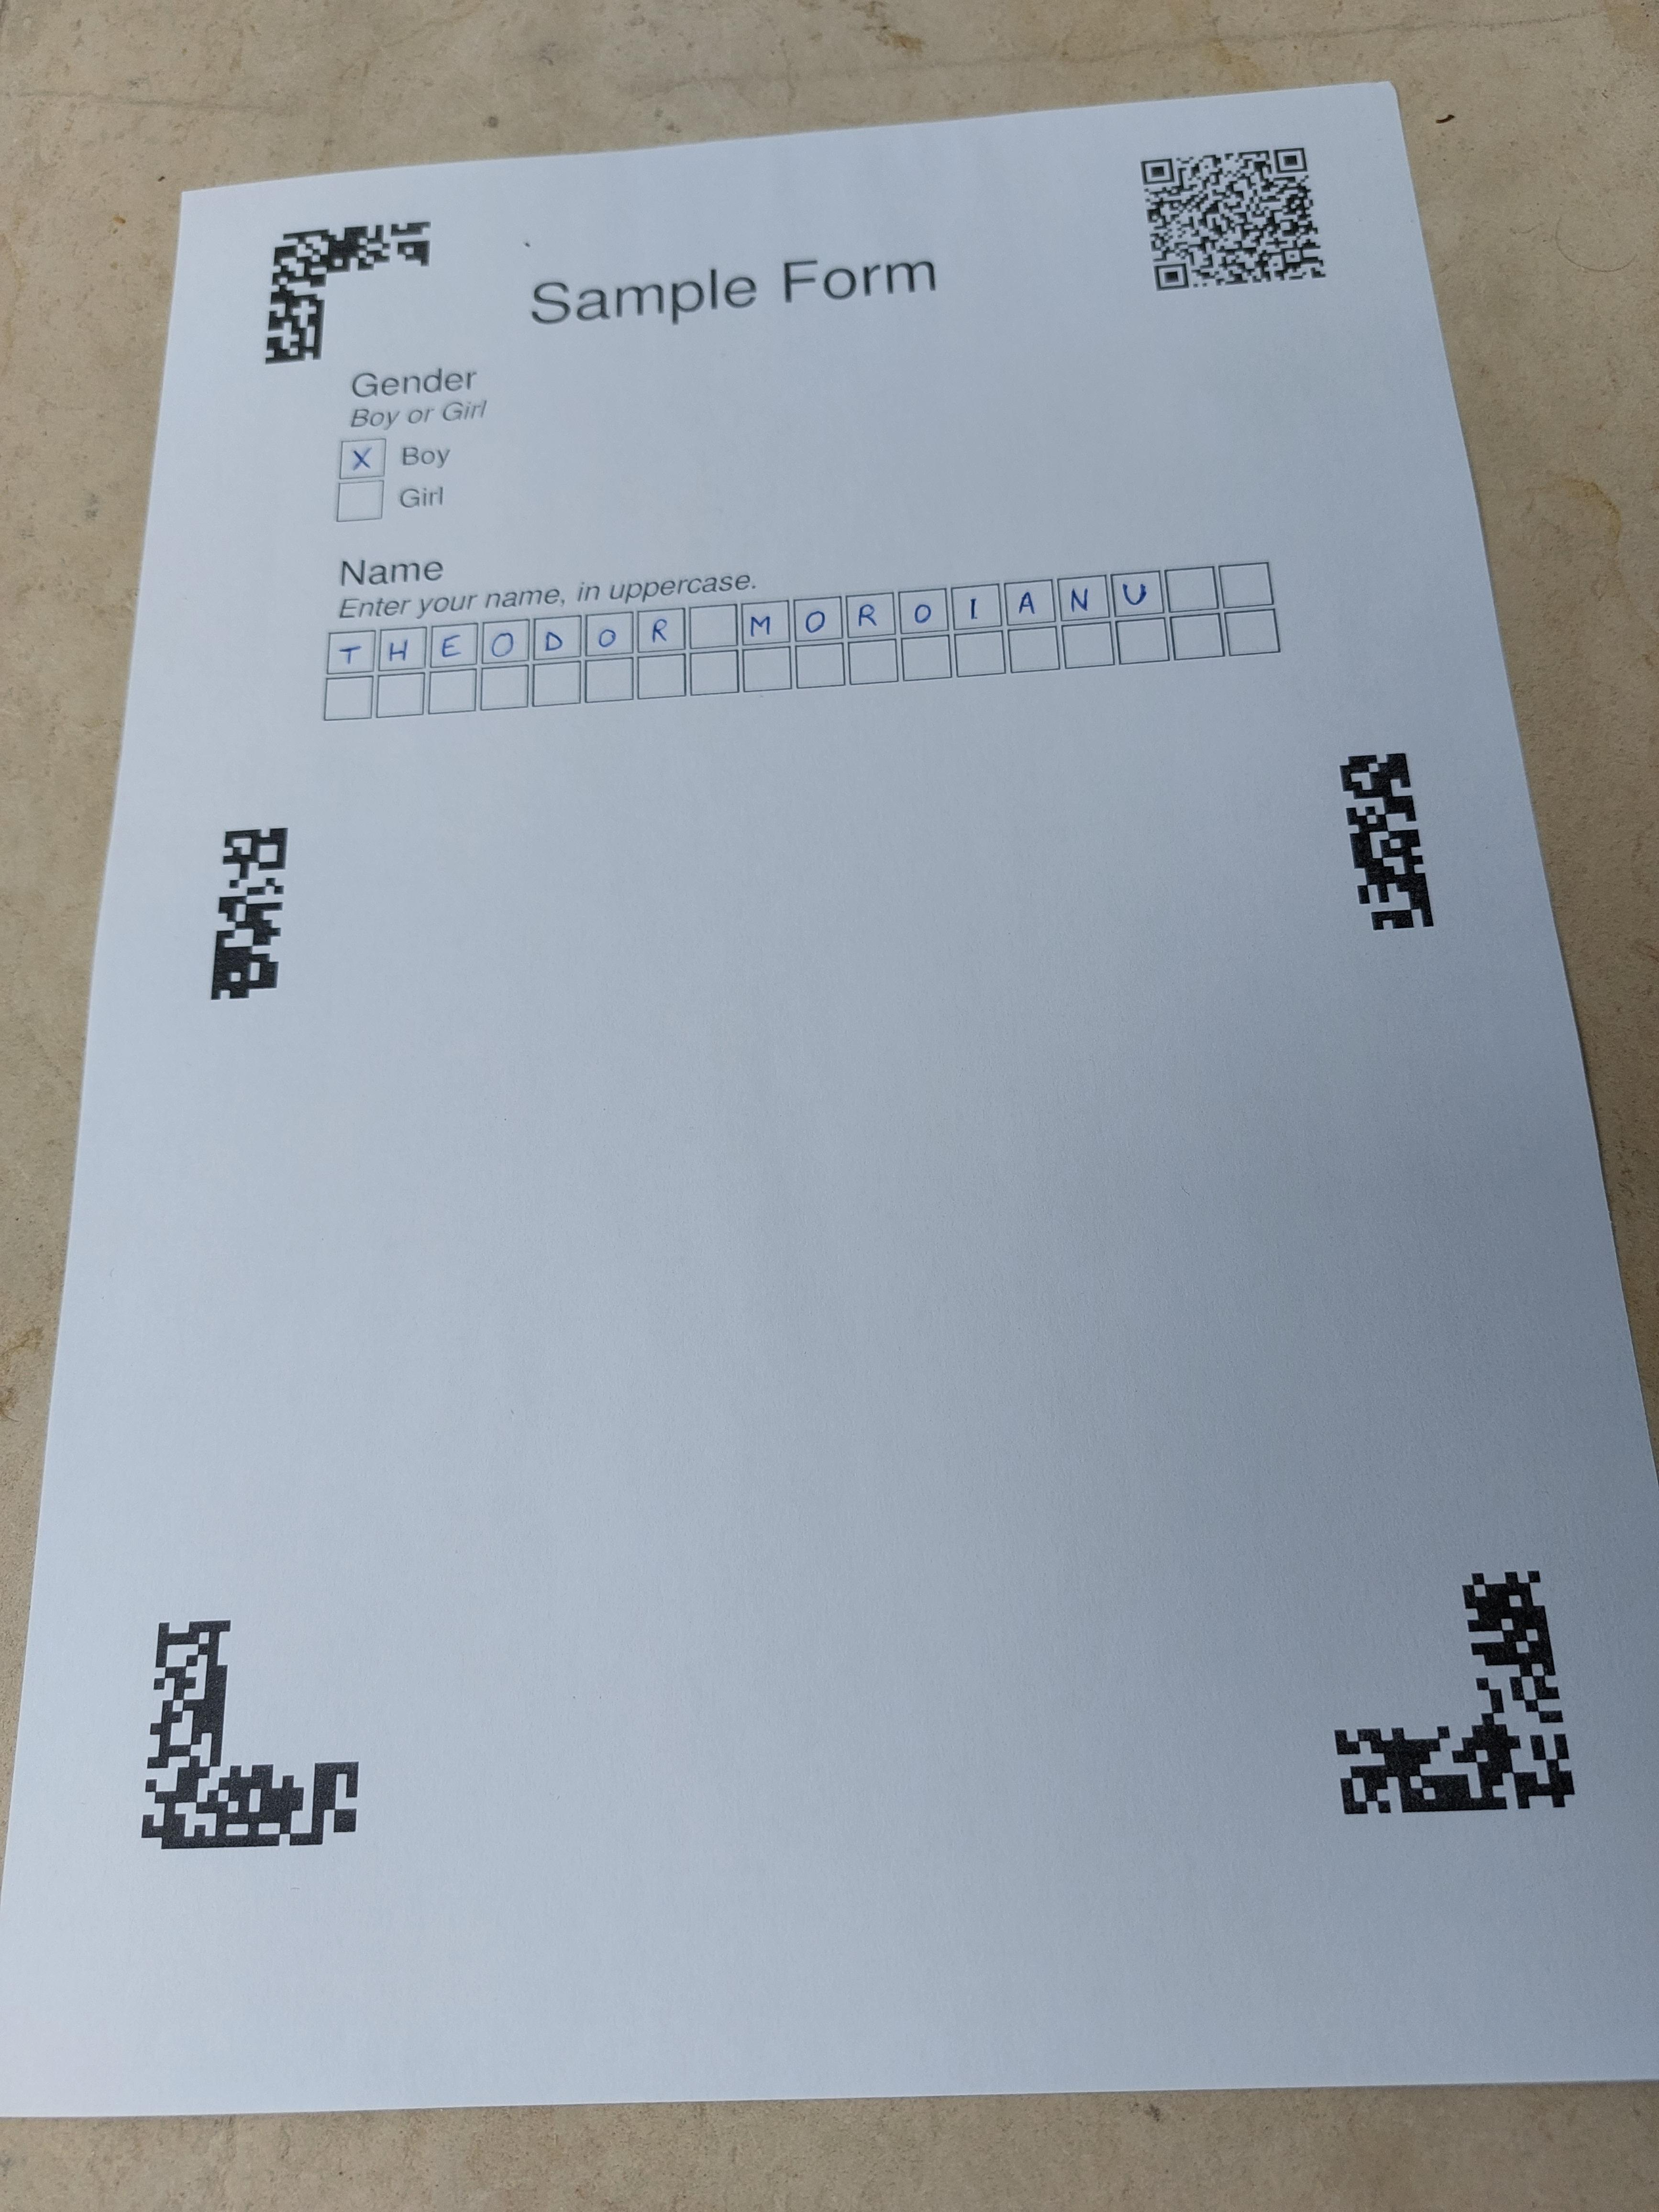
\includegraphics[width=5cm]{images/graphs/original_image.jpg}} }}%
%     \qquad
%     \subfloat[\centering label 2]{{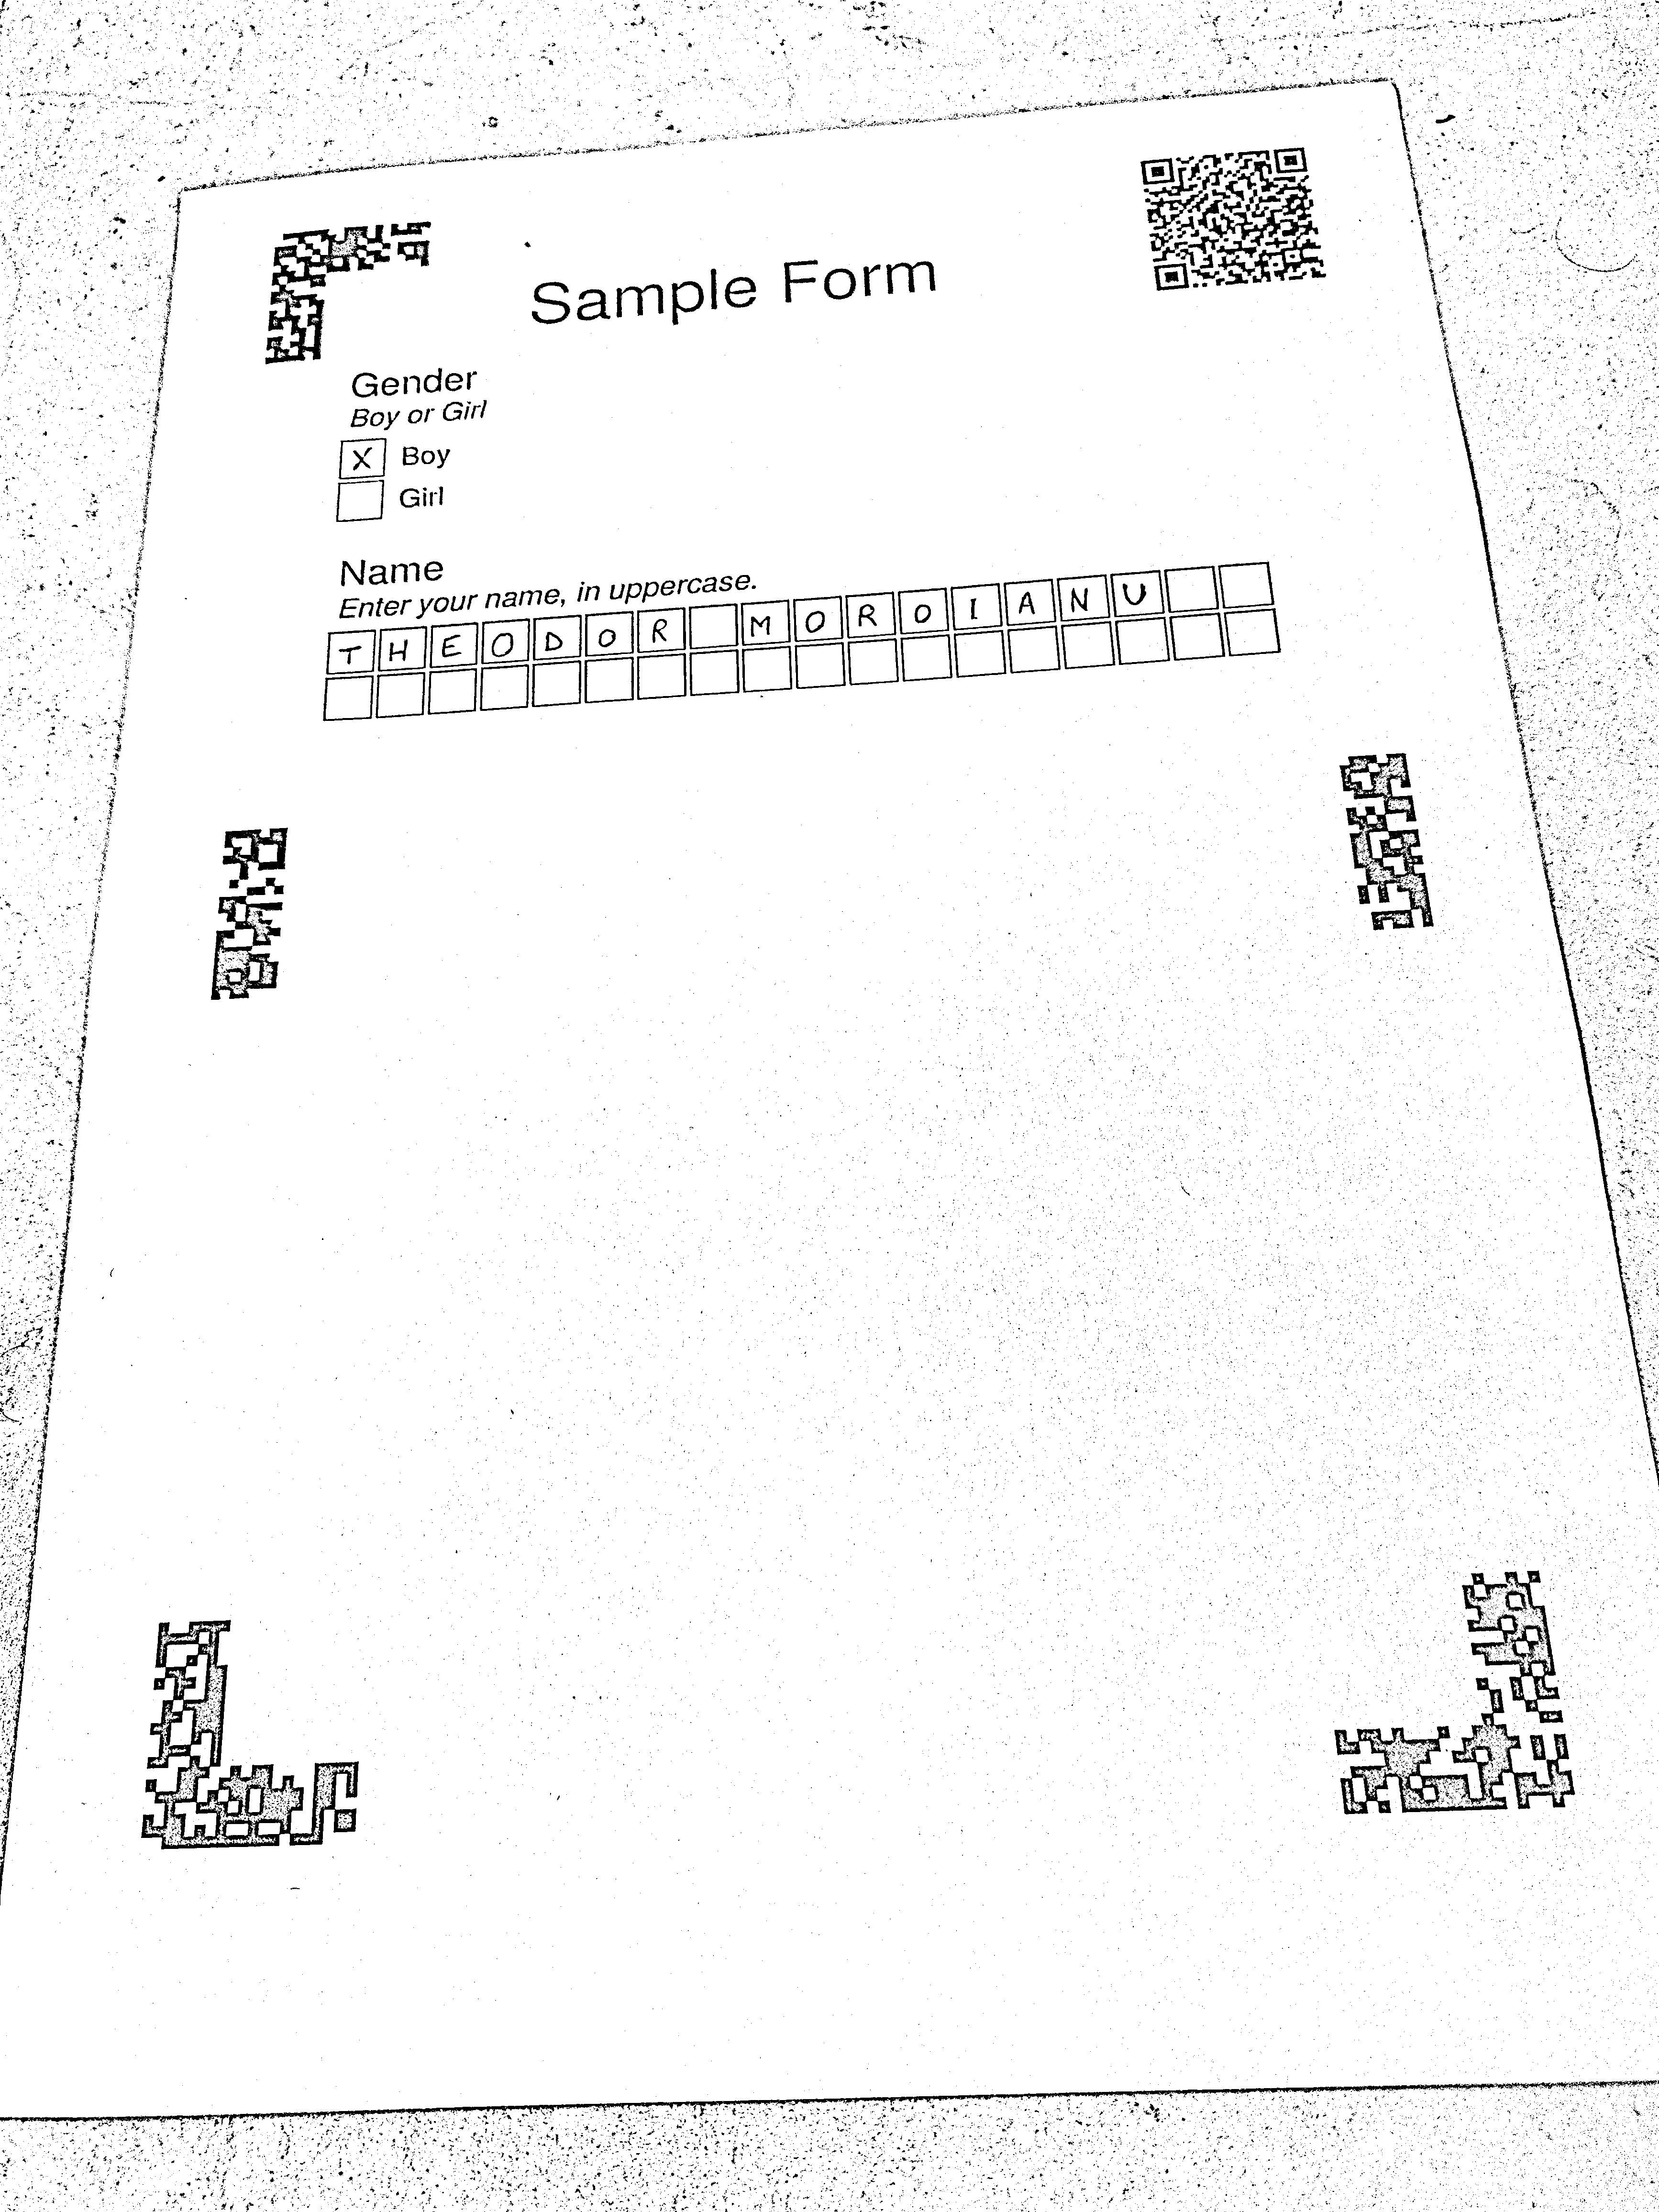
\includegraphics[width=5cm]{images/graphs/parser_processed_image.jpg} }}%
%     \caption{2 Figures side by side}%
%     %\label{fig:example}%
% \end{figure}

 \begin{figure}[!h]
     \centering
     \fbox{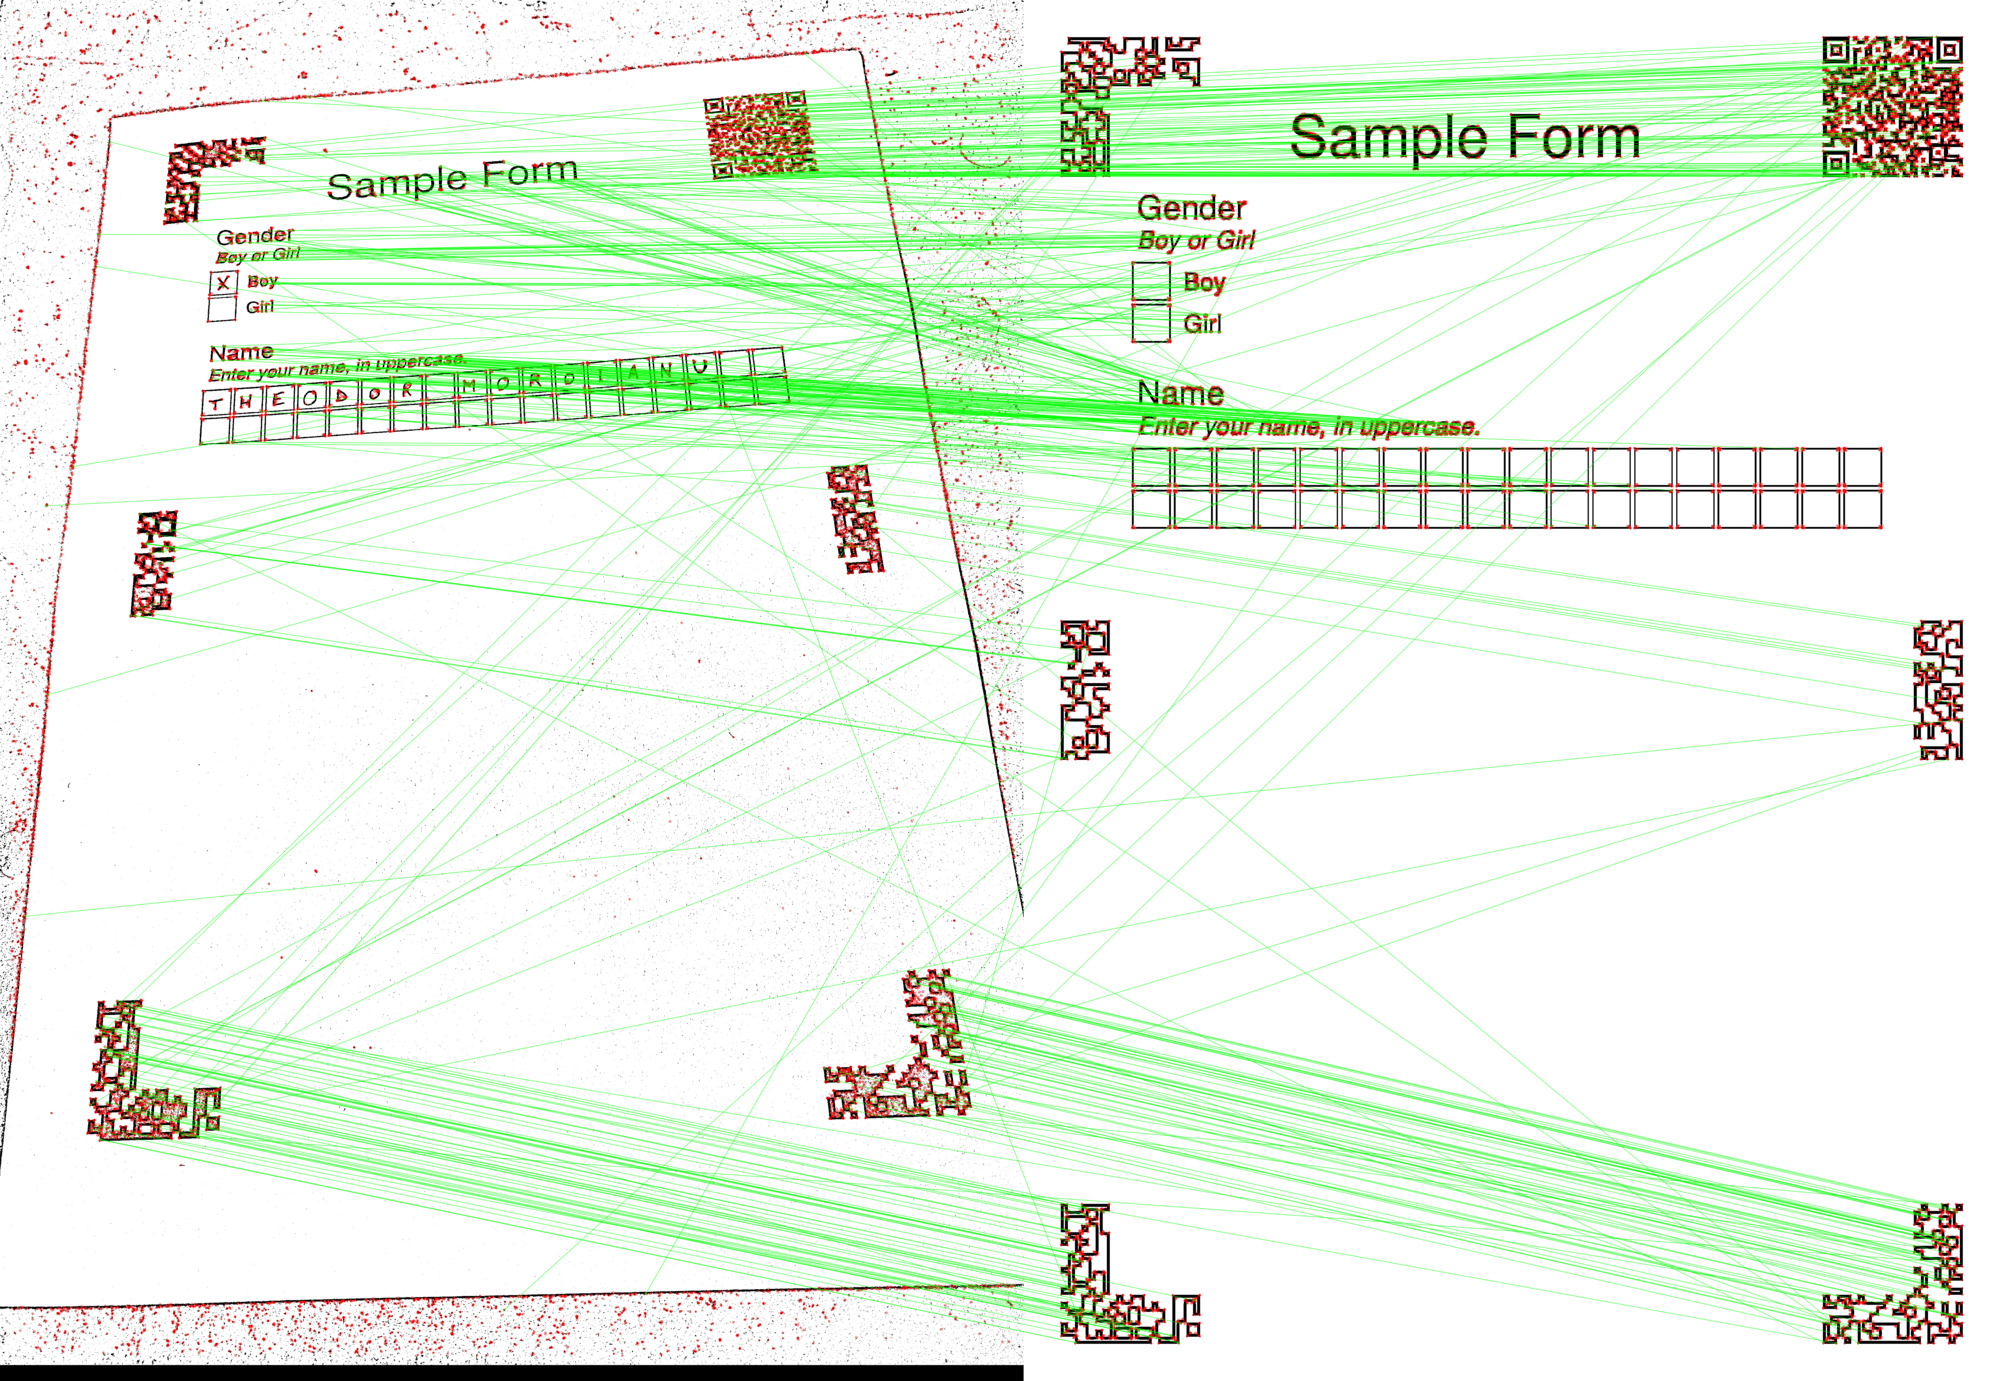
\includegraphics[width=35em]{images/graphs/parser_image_matches_fixed.jpg}}
     \caption{Matches found with ORB}
     \label{orb-matches}
 \end{figure}

For parsing the form, we have to be able to match specific pixels of the picture / scan of the form with the template, to figure out where locations we are interested in are. Further in this section, we will call the picture / scan of the form the \textit{picture}, and the original form, retrieved from the database, the \textit{template}.

Matching the picture with the template is not trivial, as things become quite messy:
\begin{itemize}
    \item If the picture keeps the same proportions, orientation and scaling as the template, then we have a perfect 1-1 match between the two.
    \item If the picture keeps the same proportions and orientation, but the scaling is not $1$, then a scaling factor is needed in order to be able to match the picture and the template.
    \item If the picture only keeps the same proportions, then in addition to the scaling factor a rotating factor is also required.
    \item If the picture does not keep the same proportions, then we have to find a homography between the two.
\end{itemize}

As finding homographies between two images is a quite common task, \textit{OpenCV} offers the ORB feature extractor\cite{rublee2011orb}, which is able to extract and match features of the two images, as seen in Figure \ref{orb-matches}. If enough matches are found, we can change the image's perspective, to get a frontal view of the form.

\begin{figure}[!h]
	\hfill
	\subfigure[Original]{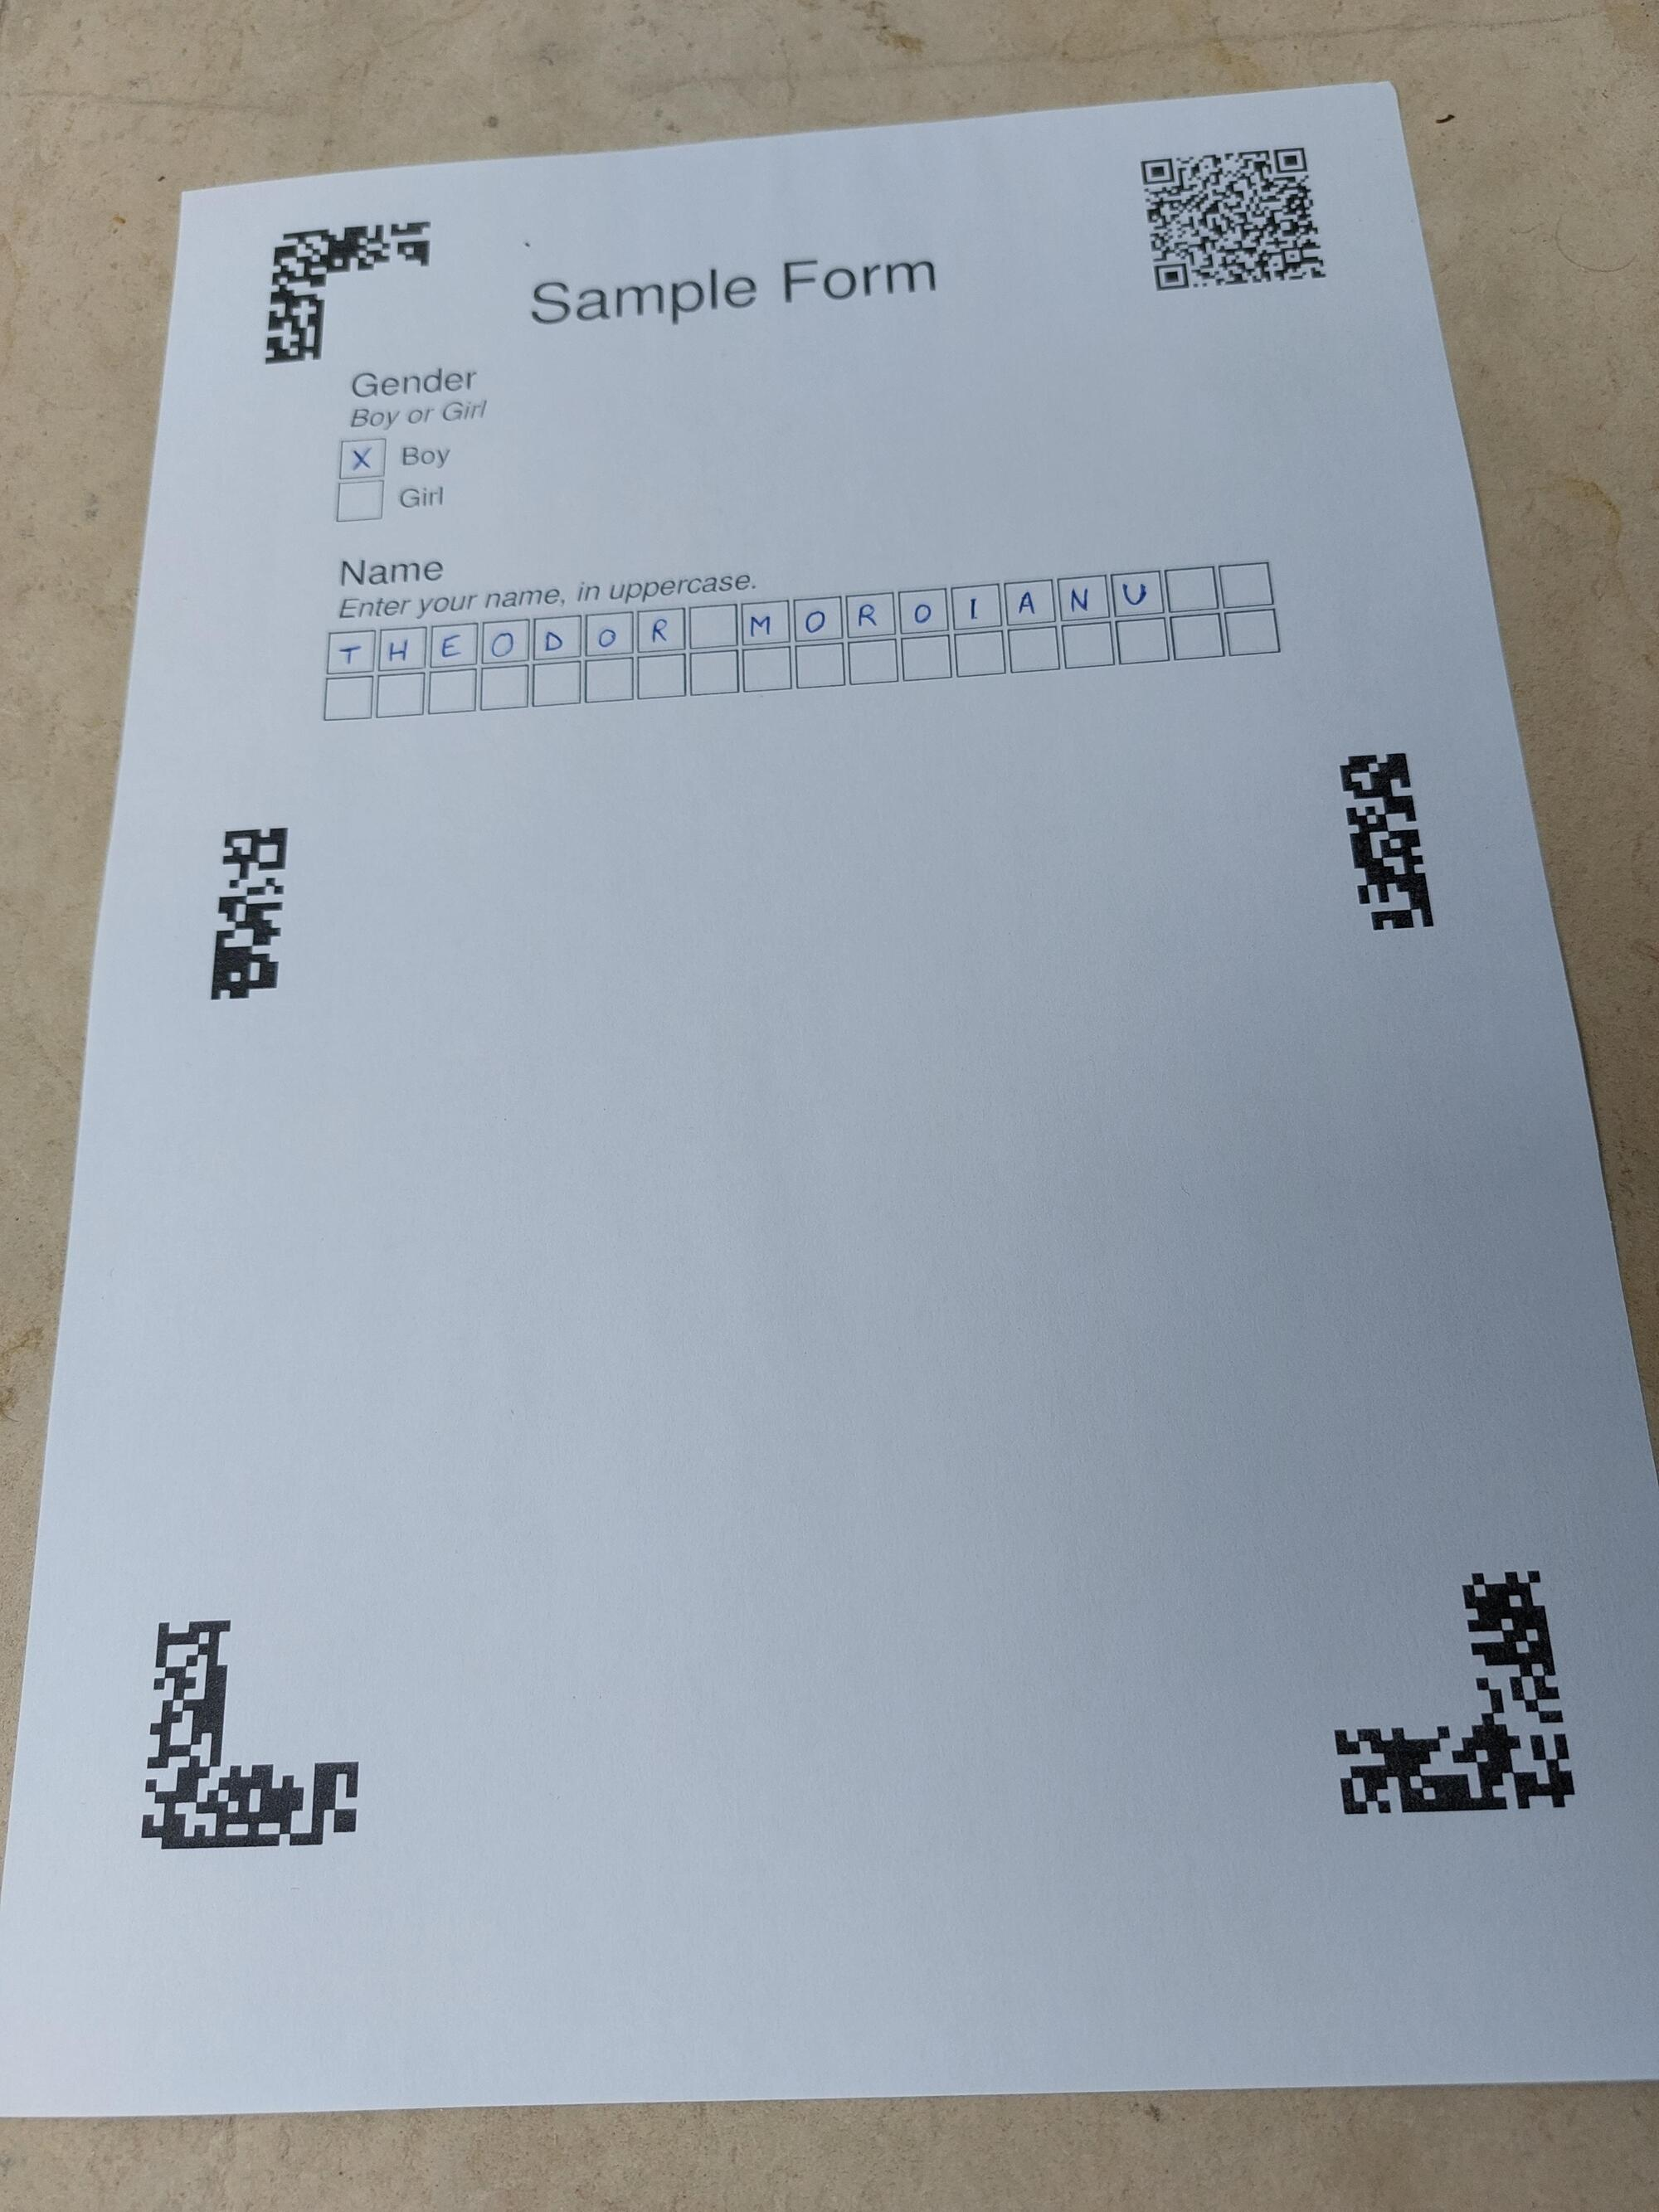
\includegraphics[height=8cm]{images/graphs/original_image_fixed.jpg}}
	% \hfill
	\subfigure[Corrected]{\fbox{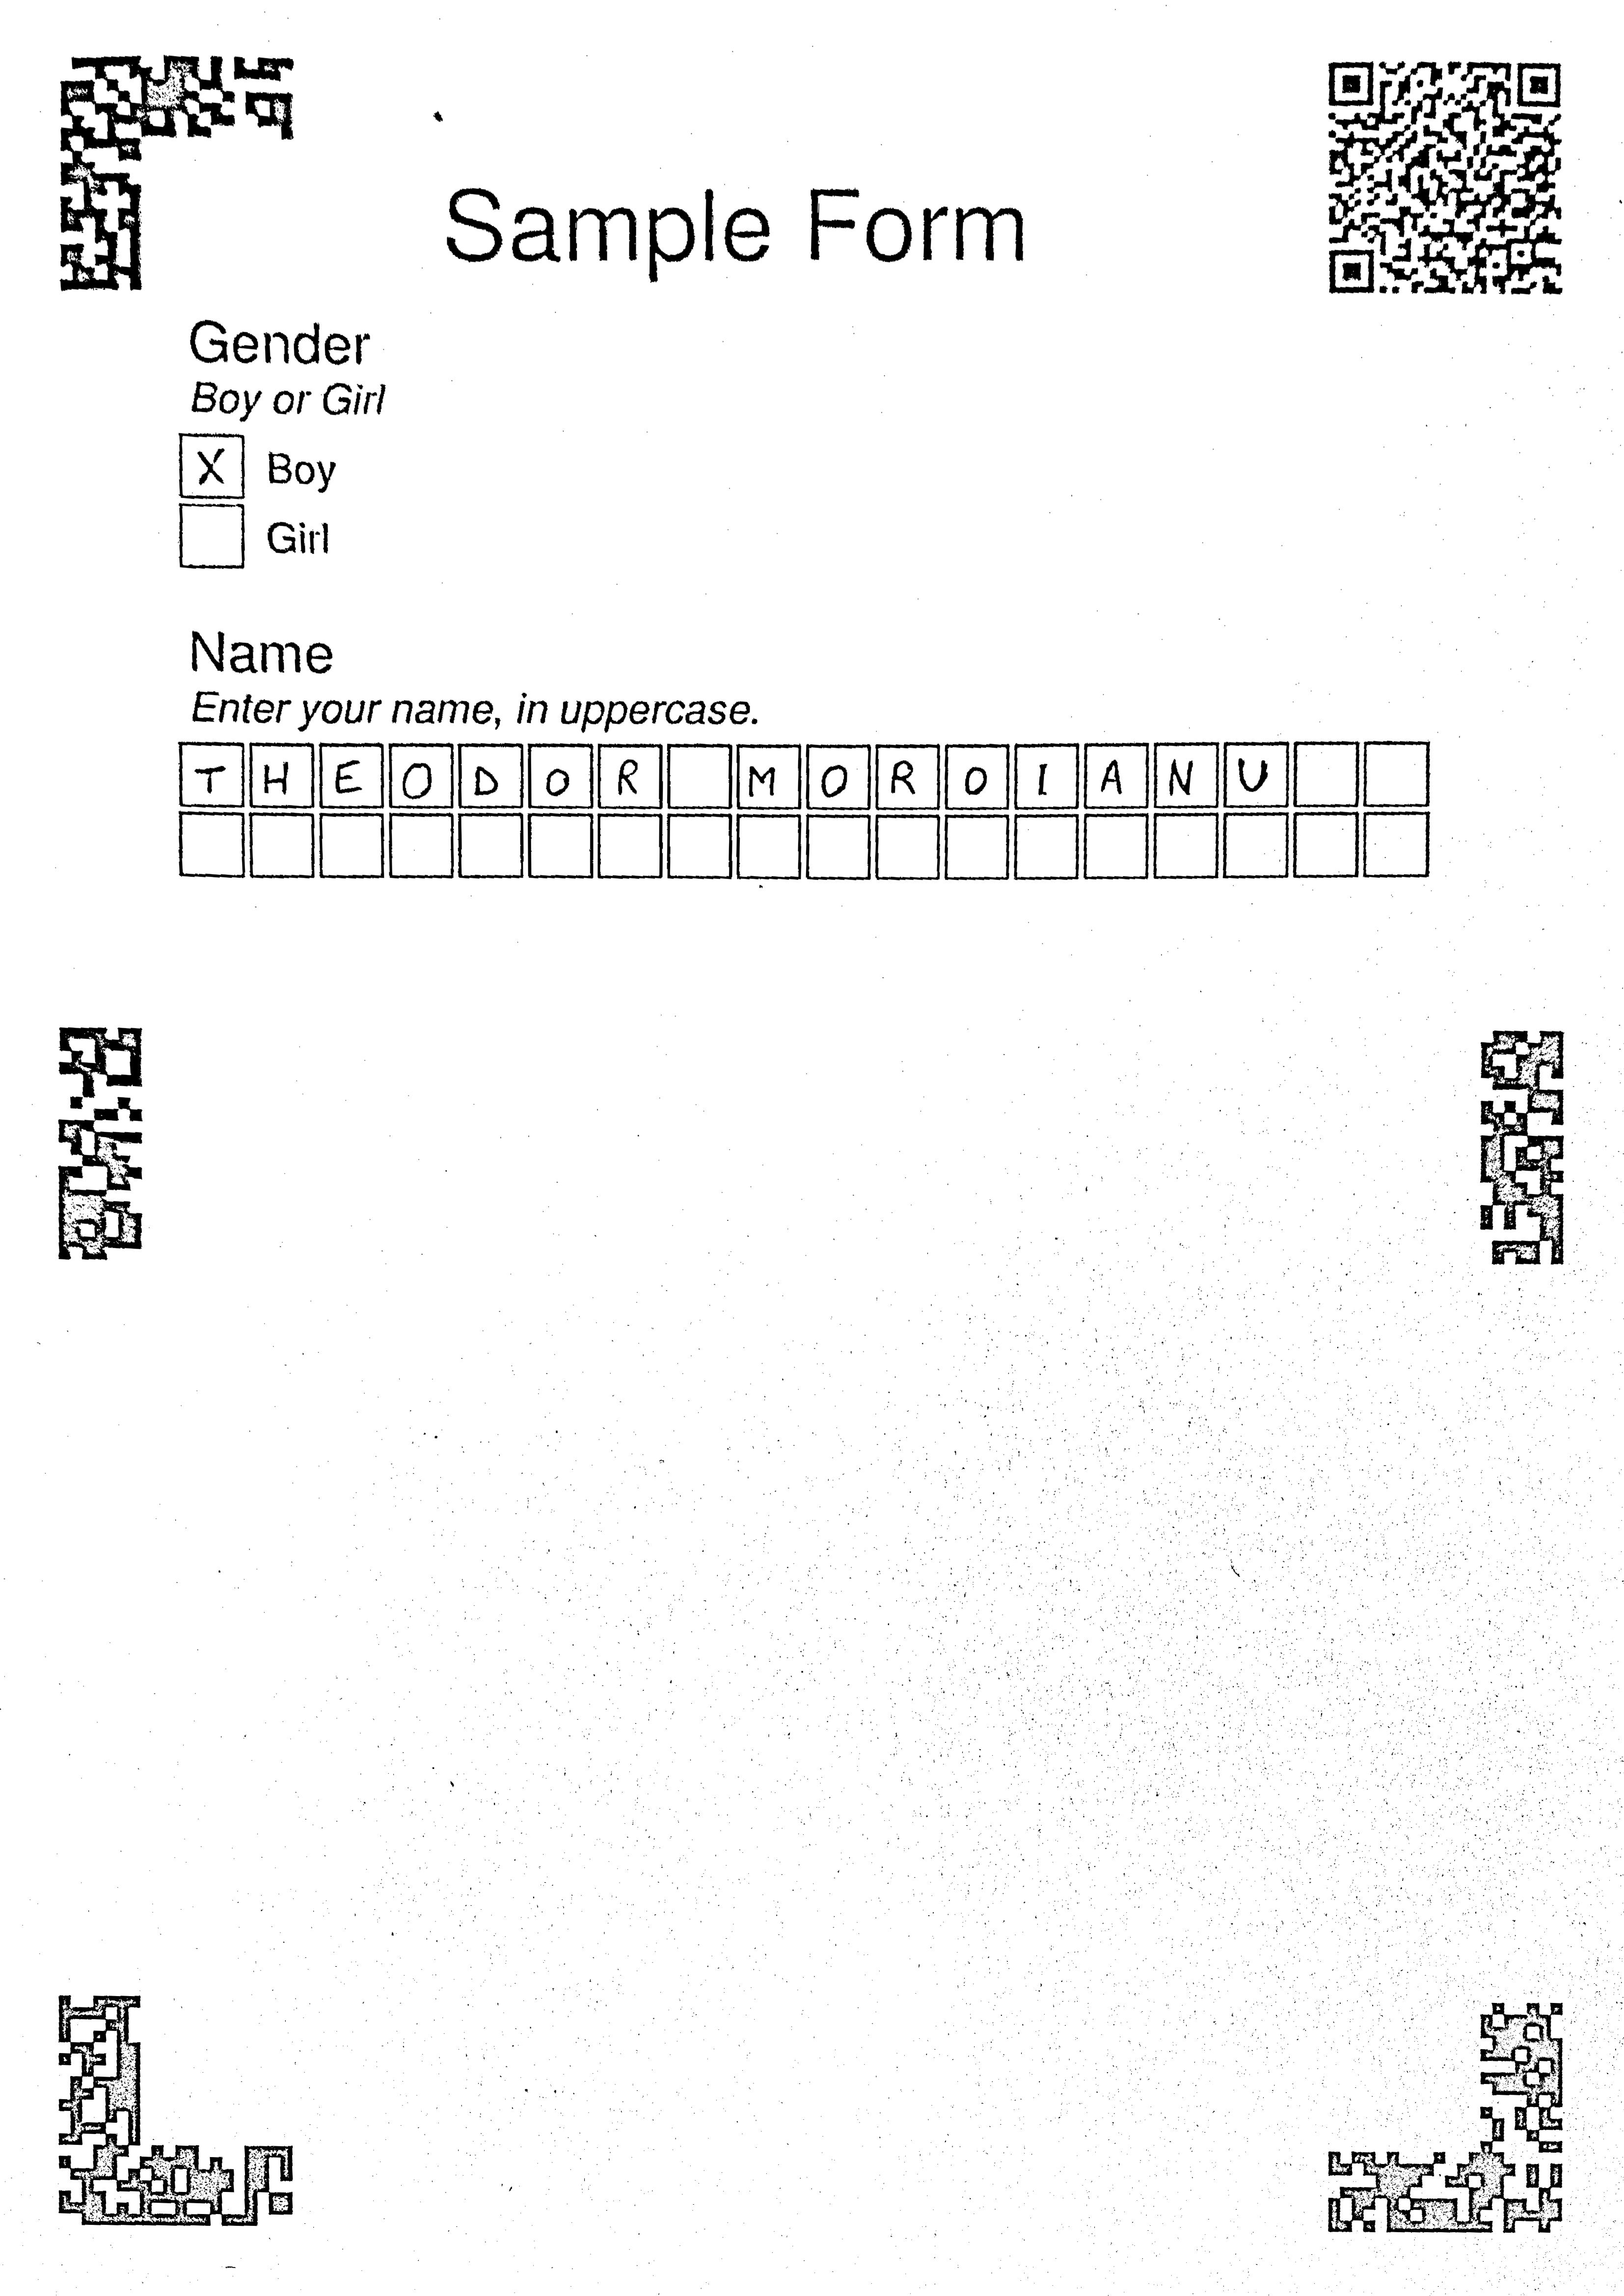
\includegraphics[height=8cm]{images/graphs/parser_corrected_image.jpg}}}
	\hfill
%	\caption{Picture converted to binary}
%	\label{original-vs-processed-image}
%	\centering
%	\fbox{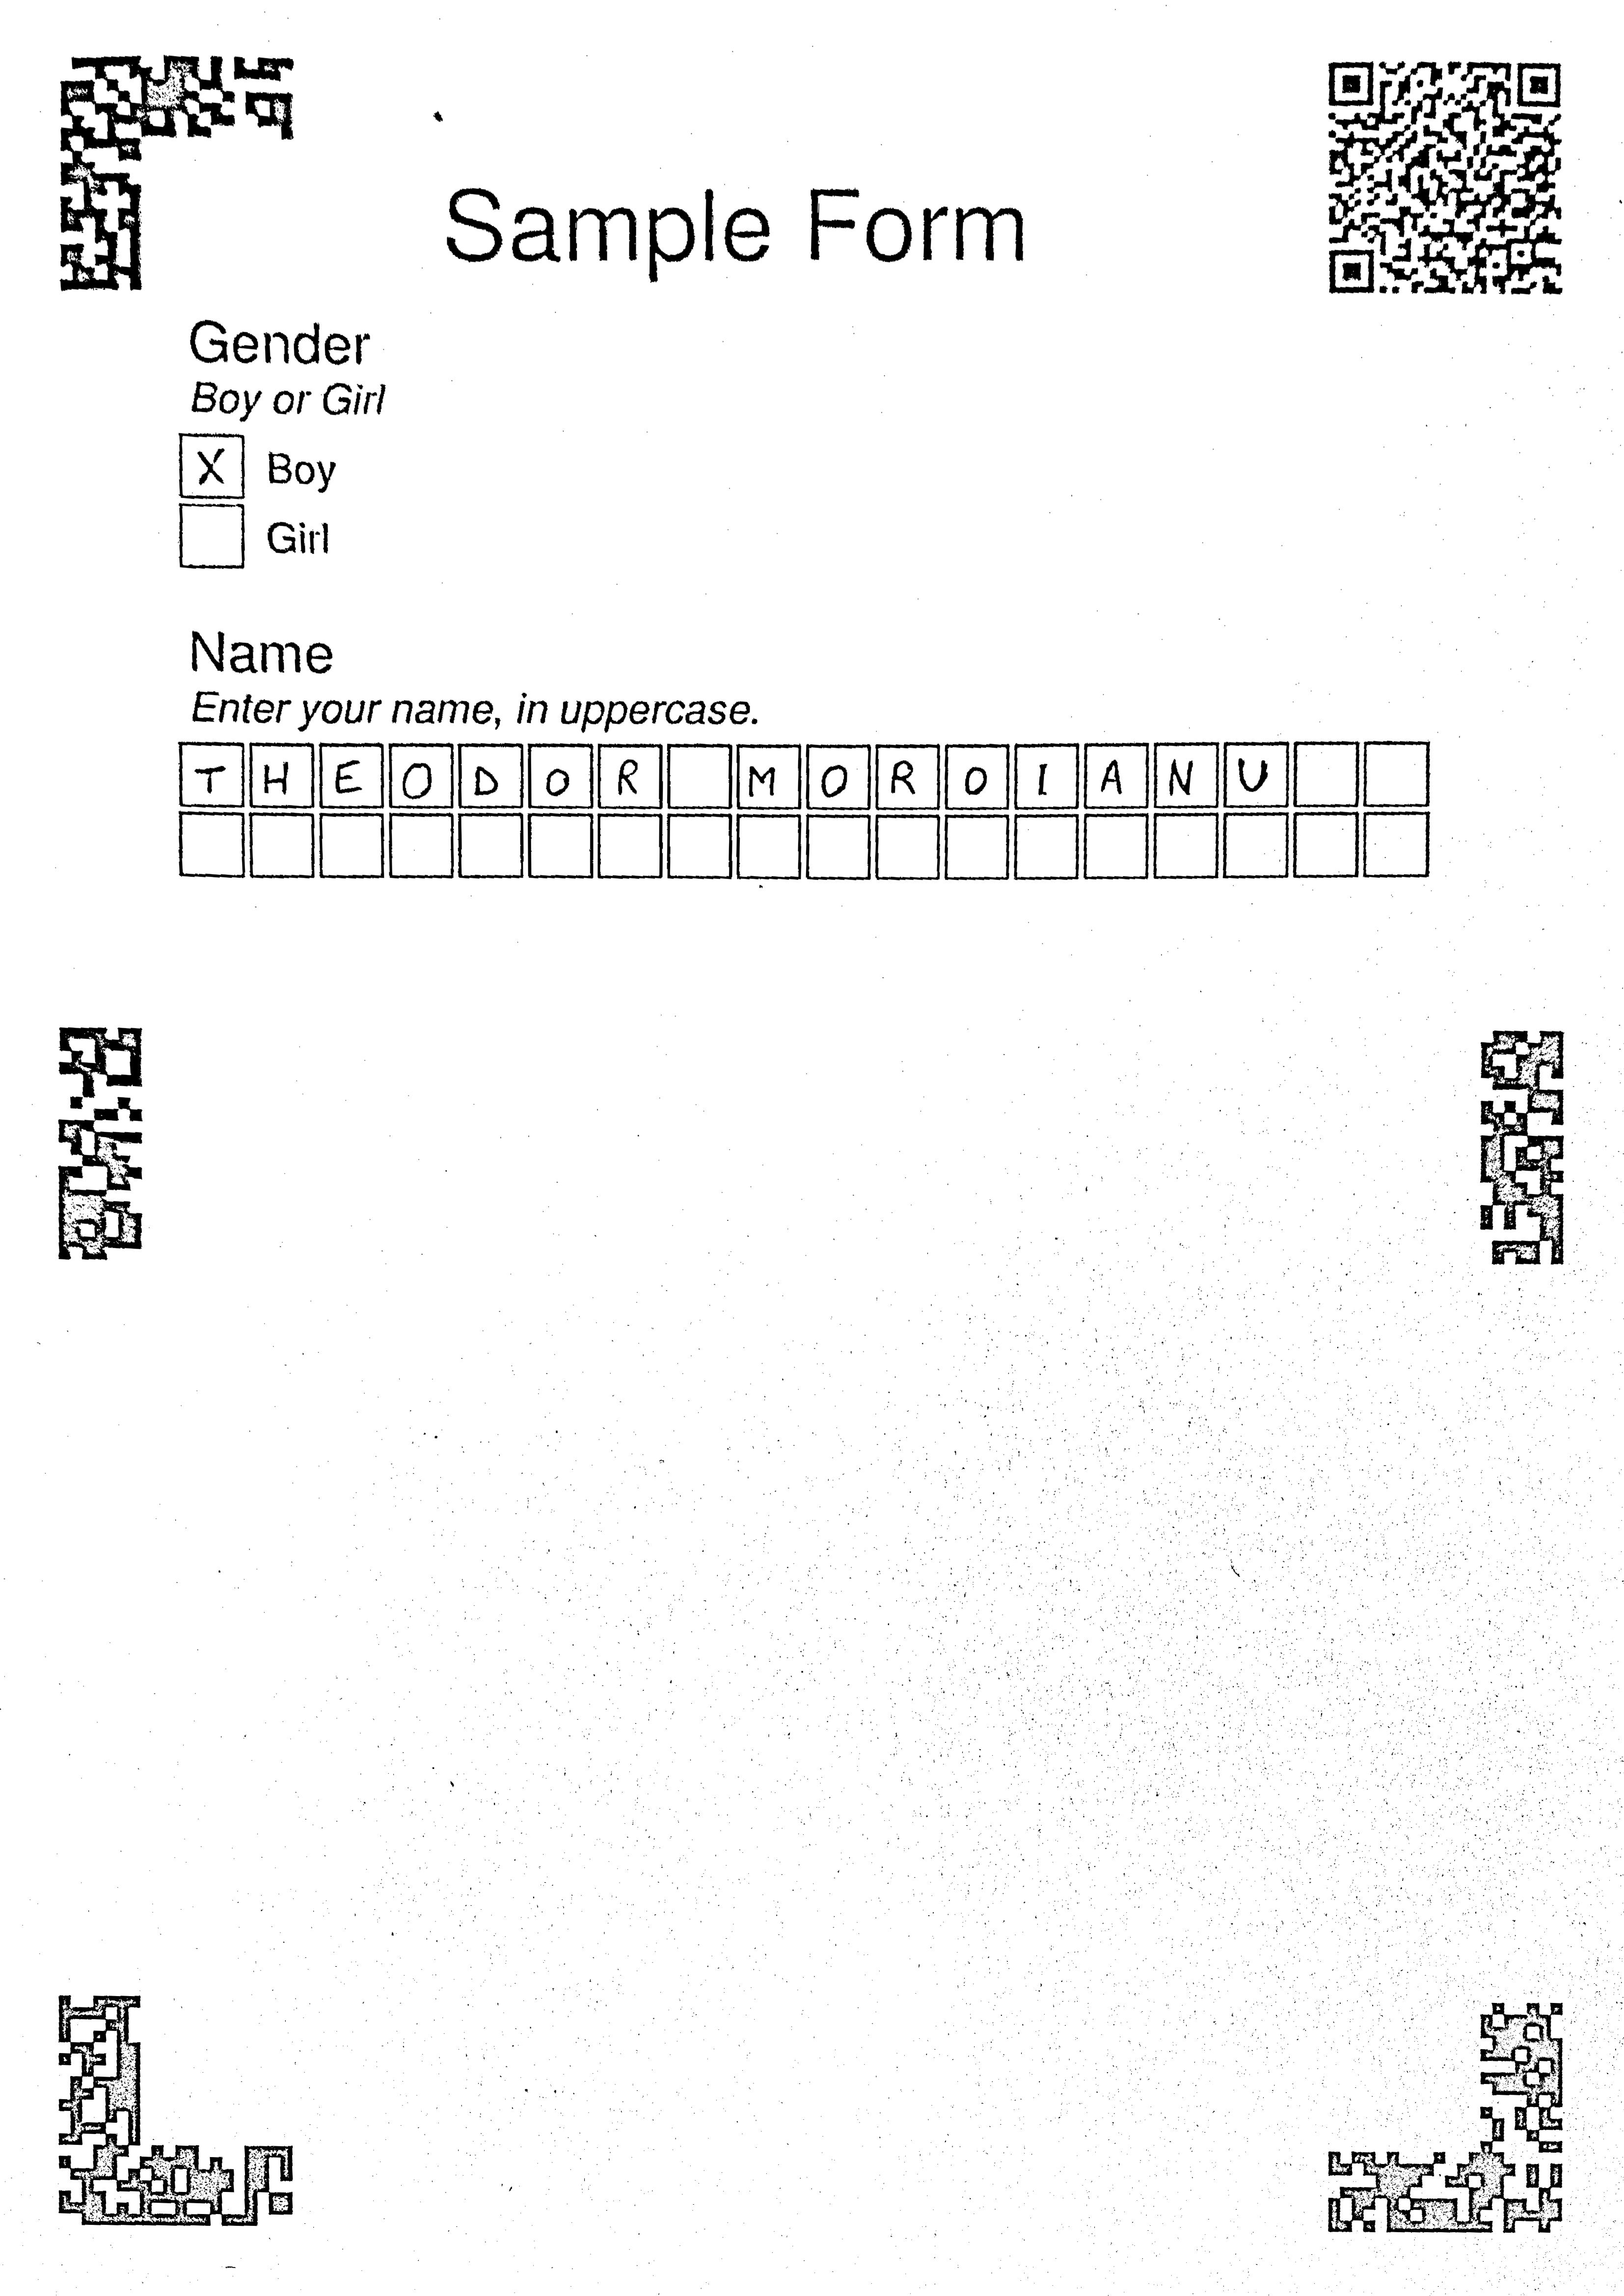
\includegraphics[width=15em]{images/graphs/parser_corrected_image.jpg}}
	\caption{Original and Corrected Picture}
	\label{parser-corrected-image}
\end{figure}

In Figure \ref{parser-corrected-image} we can see the result of our perspective transformation over the binary picture. We can observe that:

\begin{itemize}
	\item The thresholding is not perfect, as some white areas have a few black pixels, and black text has a few white spots, which means that our OCR network has to be resistant to small noise.
	\item Straight lines (more specifically the boundaries of the text boxes) seem slightly curved. This is actually the case, as phone cameras add small distorsions to the images. This fenomenon does not appear on scans though.
\end{itemize}

\section{Extracting Answer Squares}

Extracting squares containing an answer from a form is straightforward, given a corrected image. As we save the position of squares where users are writing their answers when we generate the form, we simply have to extract said square.

For each form we store in the database a list with the absolute position of each answer square. An sample of the stored information is:

\begin{minted}[bgcolor=bg]{yaml}
    answer_squares_location:
        - 0:
            - 0:
                - width: 8
                - x: 23.5
                - y: 49.5
                - page: 0
            - 1:
                - width: 8
                - x: 32.5
                - y: 49.5
                - page: 0
            ...
        - 1:
            - 0:
                - width: 8
                - x: 23.5
                - y: 89.5
                - page: 0
            ...
\end{minted}

\begin{figure}[!h]
	\centering
	\fbox{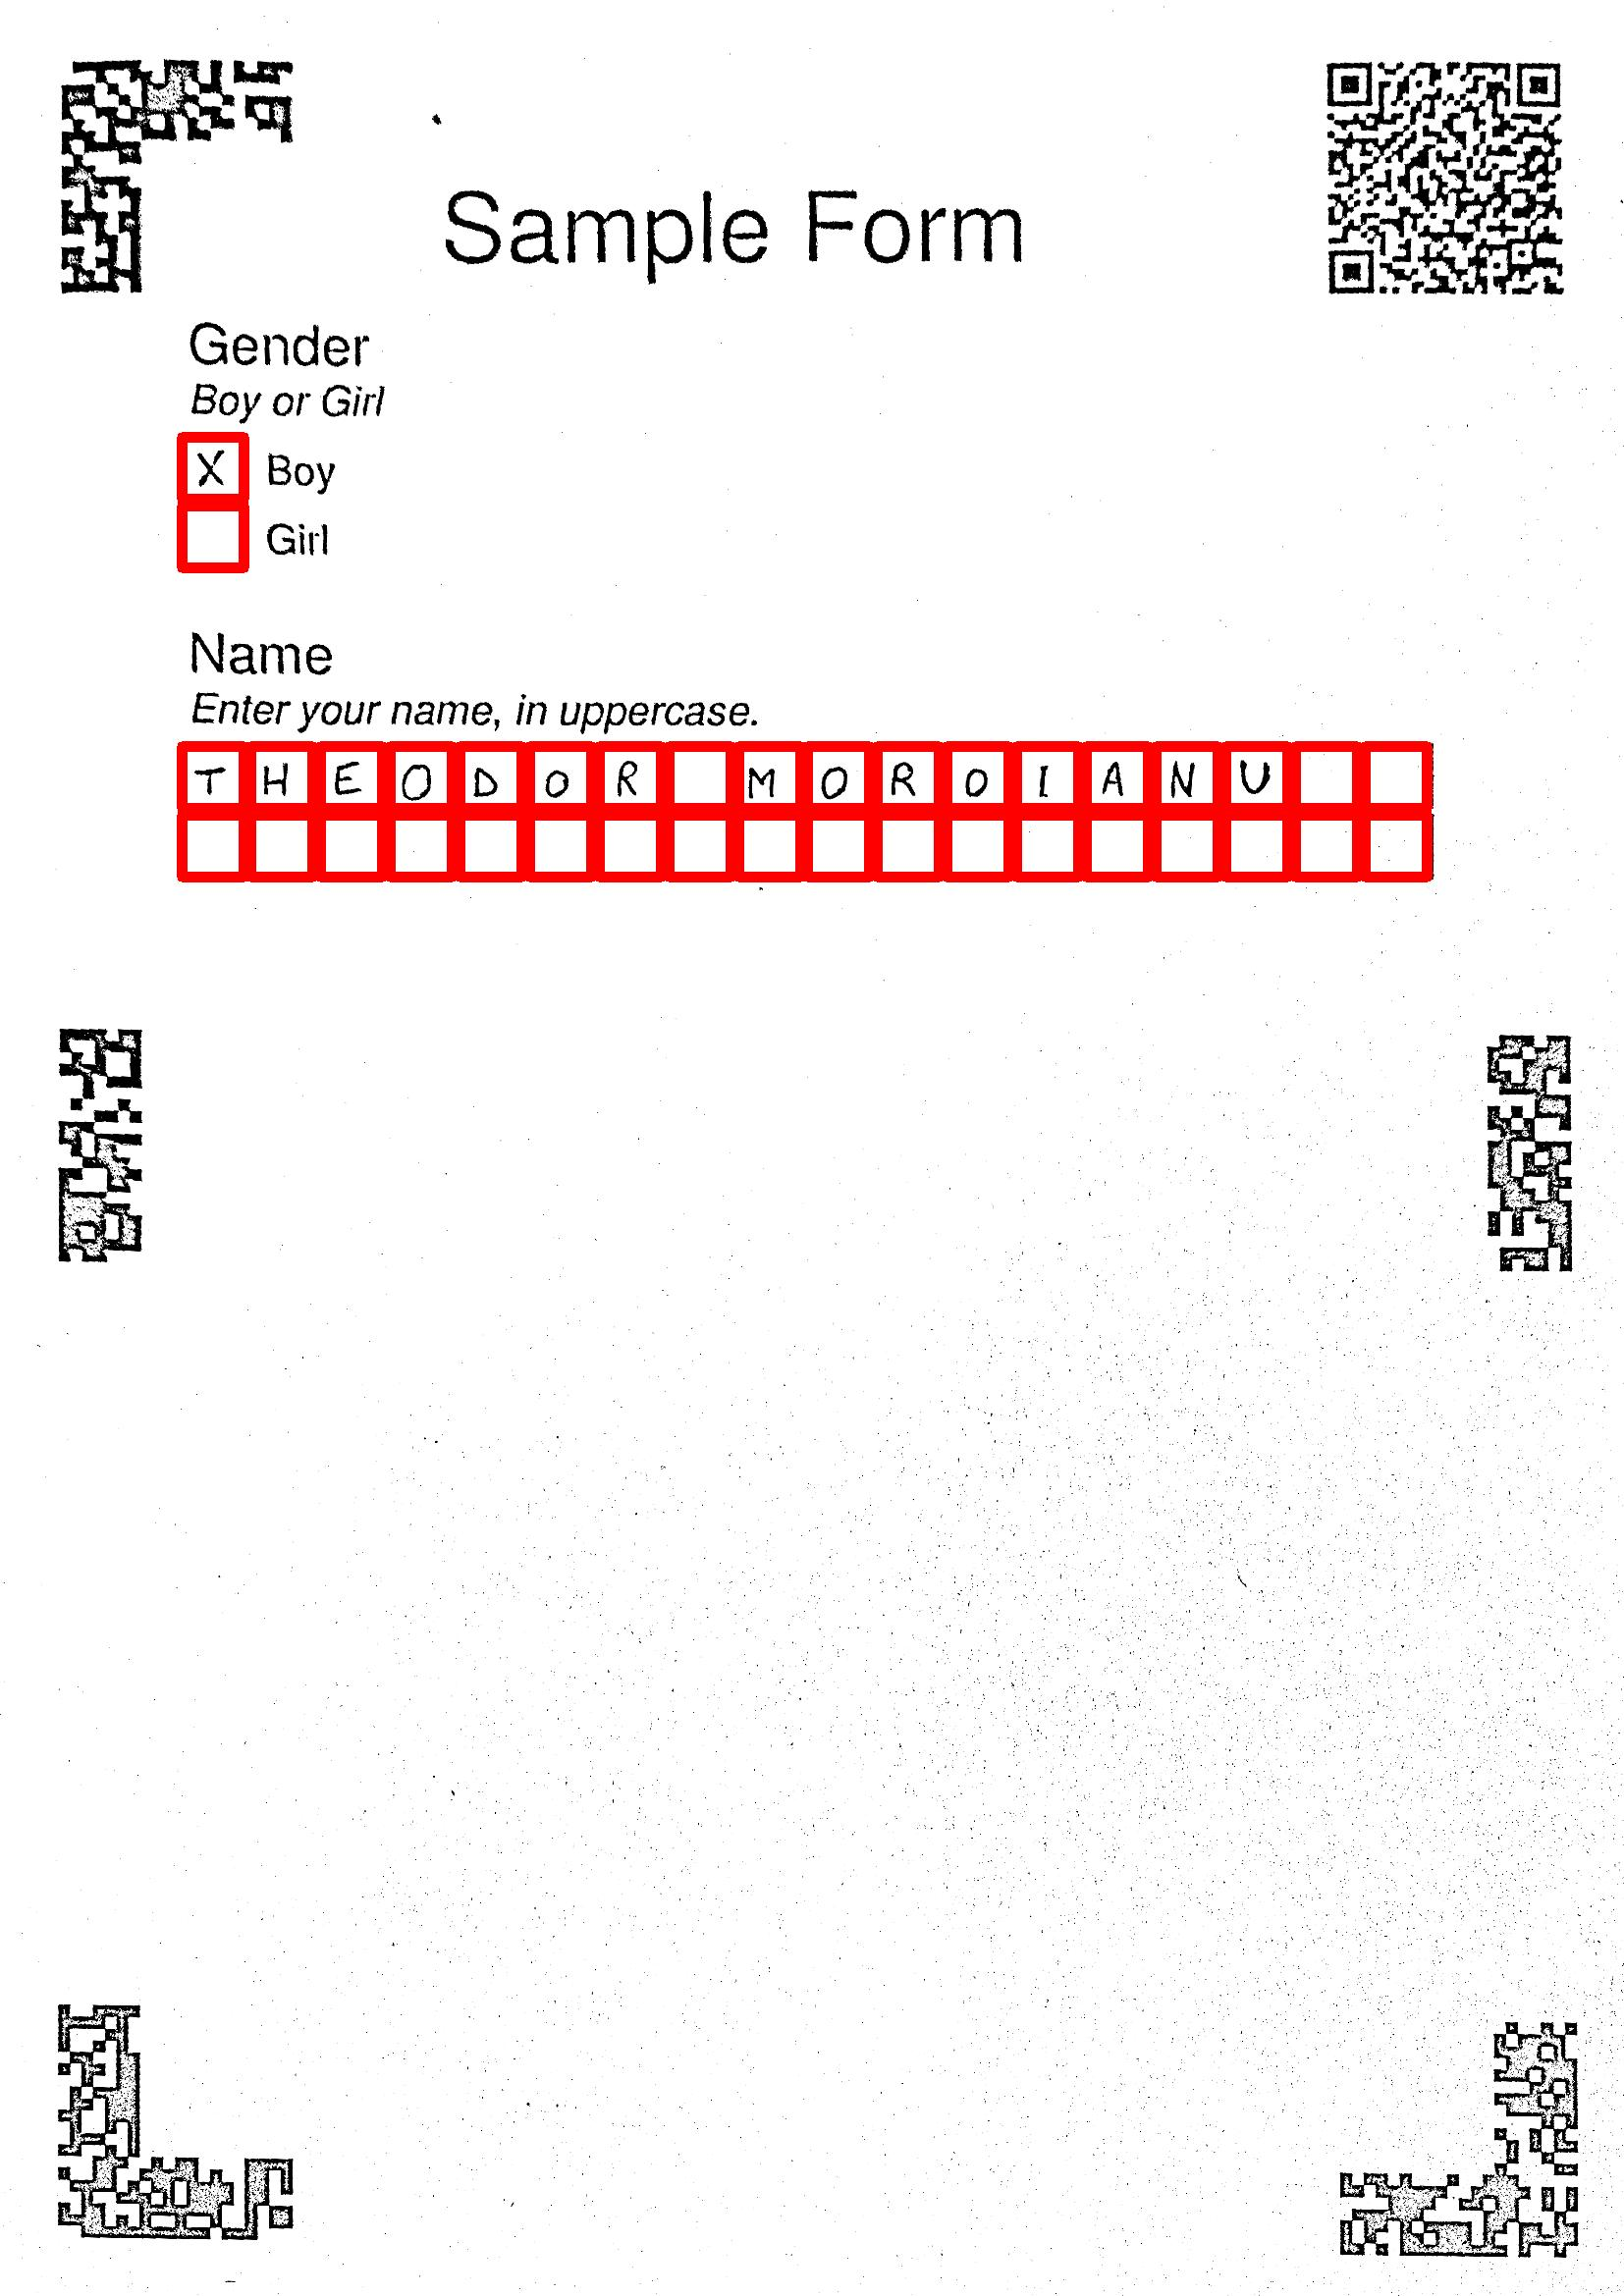
\includegraphics[width=18em]{images/graphs/fixed_image_squares.jpg}}
	\caption{Answer Squares Marked}
	\label{answer-squares-red}
\end{figure}


With the help of the information mentioned above, and of a corrected image similar to Figure \ref{parser-corrected-image}, we can mark and extract each answer square of the form. We marked in Figure \ref{answer-squares-red} the answer squares we extract in red.

Figure \ref{parsing-flow} is a flowchart of the entire parsing pipeline. As one can see, each step is independent and self-contained, which adds stability to the software and makes the source code easier to follow. 

\begin{figure}[!h]
	\centering
	\fbox{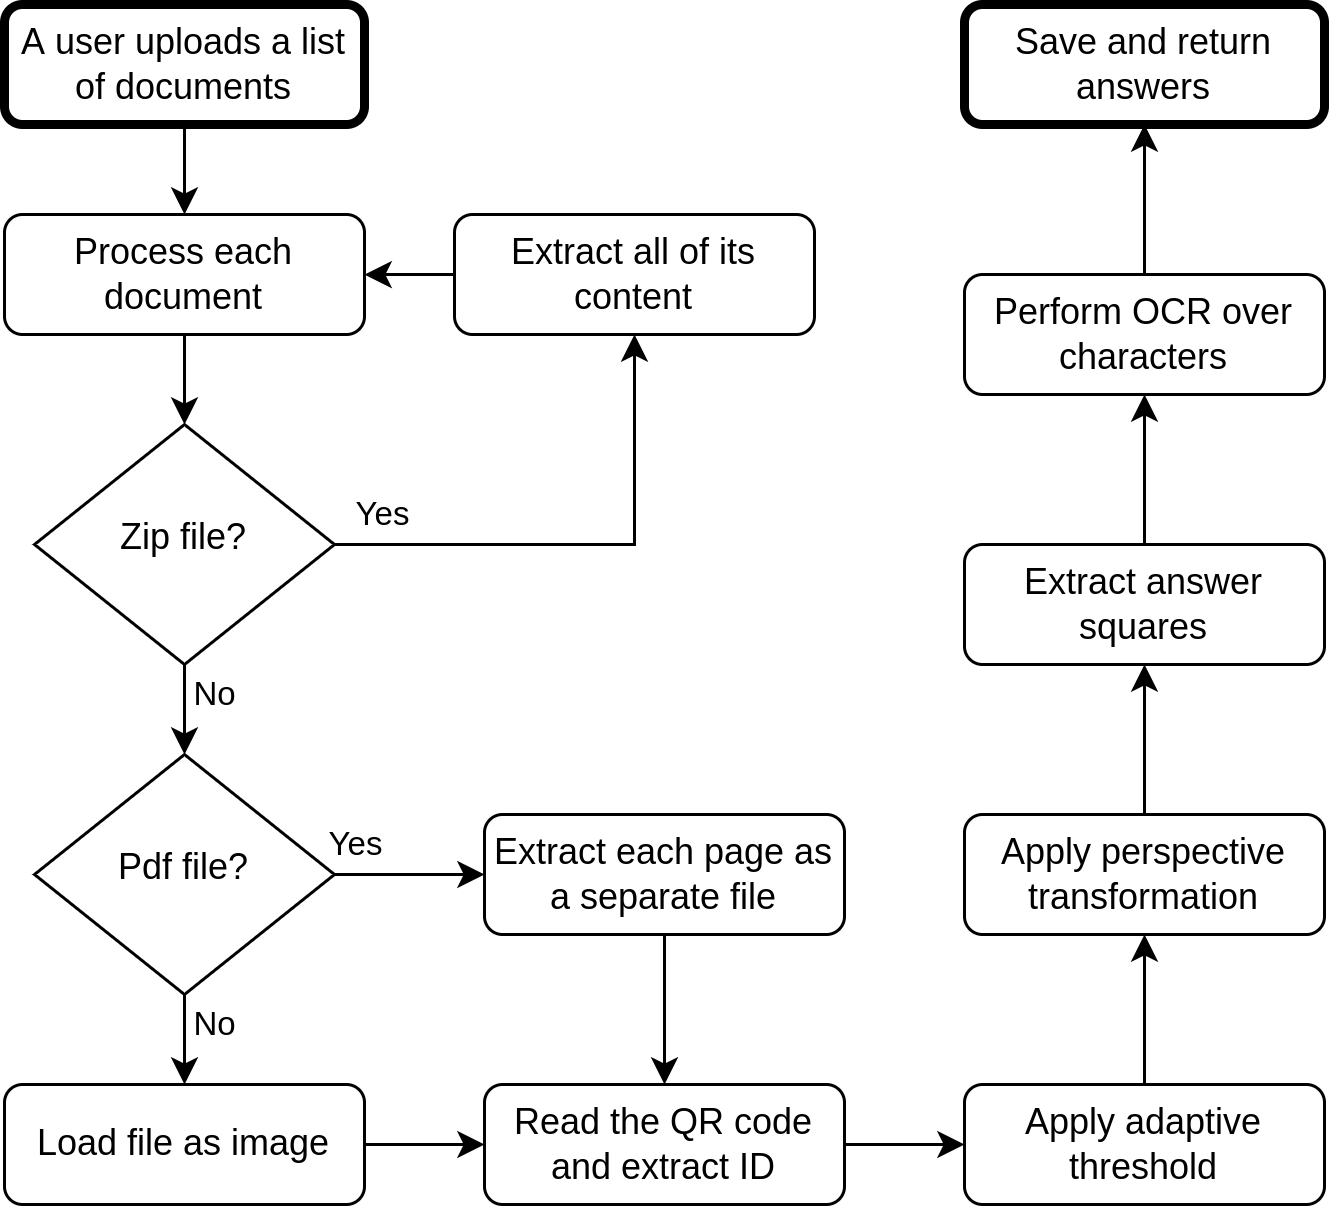
\includegraphics[width=18em]{images/diagrams/parsing-flow.png}}
	\caption{Answer Squares Marked}
	\label{parsing-flow}
\end{figure}



% cum antrenez reteaua
\chapter{OCR Neural Network Design and Training}

\section{Why Use a CNN}

We use a neural network in order to be able to extract from a small square, as the ones marked in Figure \ref{answer-squares-red}, the character written inside.

While traditional methods (such as the HOG\cite{HOG} approache) perform reasonably well, we decided to design, train and use a convolutional neural network (CNN)\cite{CNN}, as it often outperforms classic classificators.

We use \textit{Pytorch}, "\textit{an optimized tensor library for deep learning using GPUs and CPU}"\cite{pytorch}. \textit{Pytorch} allows us to design, train, save and evaluate a convolutional neural network we then use to predict characters.

\section{CNN Architecture}

We played with various common architectures, both pretrained and not pretrained, such as the \textit{VGG}\cite{VGG} or the \textit{Resnet}\cite{resnet} architectures.

However, such architectures are way to complex for our relativly simple task of classifying around $100$ characters. We ence decided to define and train our own convolutional netural network, using the \textit{Pytorch} framework.

The layers definition of our network is:

\begin{minted}[bgcolor=bg]{python}
# backend/sources/ocr/network.py
model = nn.Sequential(
    nn.Conv2d(1, 16, kernel_size=(5, 5), padding=(2, 2)),
    nn.ReLU(),
    
    nn.Conv2d(16, 32, kernel_size=(3, 3), padding=(1, 1)),
    nn.ReLU(),
    
    nn.BatchNorm2d(32),
    nn.MaxPool2d((2, 2)),
    
    nn.Conv2d(32, 64, kernel_size=(3, 3), padding=(1, 1)),
    nn.ReLU(),
    
    nn.Conv2d(64, 64, kernel_size=(3, 3), padding=(1, 1)),
    nn.ReLU(),
    
    nn.Conv2d(64, 64, kernel_size=(3, 3), padding=(1, 1)),
    nn.ReLU(),

    nn.BatchNorm2d(64),
    nn.MaxPool2d((2, 2)),

    nn.Flatten(),
    nn.Dropout(0.2),

    nn.Linear((IMAGE_SIZE // 4)**2 * 64, 1024),
    nn.ReLU(),

    nn.Linear(1024, len(CHARACTERS))
)
\end{minted}

Our network consists of:
\begin{itemize}
	\item $6$ layers of two domentional convolutions, with square kernels of sizes $3$ and $5$, over $16$, $32$ and $64$ channels.
	\item A \textit{ReLU}\cite{ReLU} activation layer after each convolution.
	\item Batch normalization and dimensionality reduction (max pools) layers.
	\item Two linear layers, acting as the classificator part of the model.
\end{itemize}

As we will show in the \textit{Training} section, this architecture is more than enough to accuratly perform our classification task. Its small size also allows it to load and run fast. The total size of the model is under $14$Mb, which, by today's standards, is really light. This allows our model to run smoothly on the \textit{CPU} as well as the \textit{GPU}, which in turn allows \textit{SmartForms} to run on low-end devices and reduces the power usage. 

\section{Dataset Used}

An easy solution to get a dataset would have been to simply create one. This has however major drawbacks:
\begin{itemize}
	\item We have to create over $62$ classes ($26 x 2$ lowercase and uppercase letters, and $10$ digits, not counting special characters such as '\code{+}', '\code{-}', spaces etc.). Making from scratch a dataset large enough to correctly train a network would be extremly time-consumming.
	\item The network is meant to recognize any handwritting. Training it on a dataset made by only two people means that characters won't have a large enough diversity to correctly generalize (different people write characters such as '\code{1}', '\code{7}', '\code{a}', '\code{e}' etc. differently).
	\item Similarly, the dataset would be dependent on the type of pen and ink used (which can have different thikness and darkness), the scanning device / phone camera model (due to post-processing all modern capturing devices do), etc. Making a robust dataset would mean spending a lot of time, effort and money in using as many different parameters as possible. 
\end{itemize}

To fix this issue, the obvious solution is to use an already made dataset.
The dataset we choose to use is the \textit{EMNIST}\cite{emnist} dataset, which contains over $500000$ handwritten letter, lowercase and uppercase letters. Sadly we were unable to find a dataset containing non-alphanumeric characters.

To account for whitespaces, we enhanced the EMNIST dataset with $10000$ peppered (with random black noise) blank images. This is necessary as the network needs to be able to detect if a certain square contains or not a character.

For optimization reasons, we processed the entire dataset once, resizing images to the size our network expects as input, and adding whitespaces. A small snippet of code showing an overview of the dataset extraction is the following:


\begin{minted}[bgcolor=bg]{python}
# backend/sources/ocr/generate_dataset.py

images: np.ndarray, labels: np.ndarray = [], []

# importing and loading the entire dataset
import tensorflow_datasets as t_d
ds = t_d.load('emnist', split='train', shuffle_files=True)

# resizing images from the dataset and adding them
# to the `images` and `labels` lists
# [...]

# generating a list of 10000 blank images
# and adding them to the `images` and `labels` list
whitespaces = []
for i in range(10000):
    whitespaces.append((np.zeros((28, 28), dtype=np.uint8), 62))
# [...]

# saving the entire dataset as a numpy binary file
# at the location `DATASET_PATH`
os.makedirs(DATASET_PATH)

imgs = np.stack(imgs)
labels = np.stack(labels)

np.save(IMAGES_PATH, imgs)
np.save(LABELS_PATH, labels)
\end{minted}

\section{Data Processing and Augmentation}

The main issue we had to fight against is that images from the EMNIST dataset do not look completly similar. This means the data we train on is not the same as the data we want our model to predict.

To fix this issue, we heavily rely on data augmentation and post-processing. The augmentation techniques we use are:
\begin{itemize}
	\item Image erosion and dilation (increasing / reducing the white zone).
	\item Image resizing -- randomly cropping borders of the images or padding it, essentially zoomin into / out of the image.
	\item Random translations. This is especially usefull as most EMNIST data is perfectly centered in the image, but ours is not.
	\item Random rotations by a relatively small angle.
	\item Salt and pepper random noise.
\end{itemize}

For post-processing, we apply the Canny edge detector, which returns a smoothed contour of the image. After applying data augmentation on the EMNIST dataset and post-processing on both EMNIST and our images we found no visual difference between the two, and, based on a small handmade dataset, the accuracy of our model is similar.
 


\begin{figure}[!h]
	\begin{center}
%		\hspace{1cm}
		\subfigure[Raw Data]{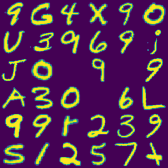
\includegraphics[width=5cm]{images/graphs/raw-emnist-data.png}}
%		\hfill
		\hspace{1cm}
		\subfigure[Augmented Data]{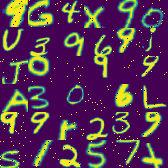
\includegraphics[width=5cm]{images/graphs/augmented-emnist-data.png}}
%		\hspace{2cm}
		\\
%		\hspace{1cm}
		\subfigure[Processed Raw Data]{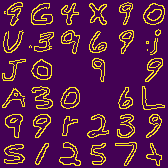
\includegraphics[width=5cm]{images/graphs/processed-emnist-data.png}}
%		\hfill
		\hspace{1cm}
		\subfigure[Processed Augmented Data]{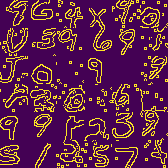
\includegraphics[width=5cm]{images/graphs/processed-augmented-emnist-data.png}}
%		\hspace{1cm}
	\end{center}
	\caption{Data Augmentation of the EMNIST dataset}
	\label{emnist-transformation}
\end{figure}

In Figure \ref{emnist-transformation} we can see the different stages of pre-processing of our dataset. We train the network on the processed augmented data (d), but validate against and expect real world data to be similar to (c). Blank characters represent whitespaces (' ').

\section{Training}

We trained the network using the standard \textit{Pytorch} method (defining a loss function, an optimizer, and looping throughout mini-batches to train the network).

The classification task we want our model to perform is ambiguous (for e.g., '\code{o}', '\code{O}' and '\code{0}' are written similarly). To counter this issue, we define a \textit{per-class accuracy}, where for a given character we only consider characters in the same class (digits, lowercase or uppercase) -- note that whitespaces are considered to belong to all $3$ classes. In other words, a given character is corectly determined in our \textit{per-class accuracy} metric iff the corect label has the highest score among all characters of the same class.

This metric is the one we are interesed in, as questions we have to parse contain a list of allowed characters set by users (for instance, a phone number field will only allow digits). The network obtains an error rate of less than $1.5\%$, with which we are confortable, as the misclassified characters are for the most part badly written characters. Figure \ref{ocr-results} shows the evolution of loss and accuracy over the training. 


\begin{figure}[!h]
	\begin{center}
		\subfigure{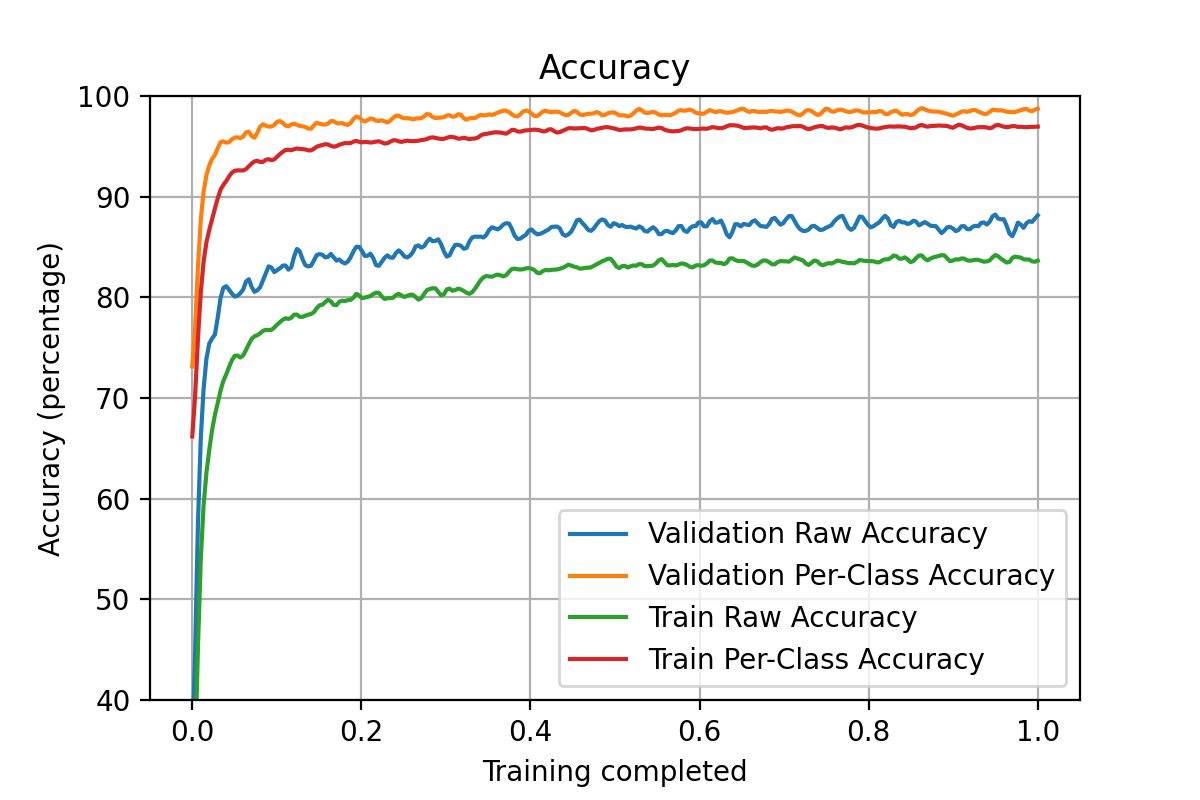
\includegraphics[width=10cm]{images/ocr/accuracy.png}}
		\\
		\subfigure{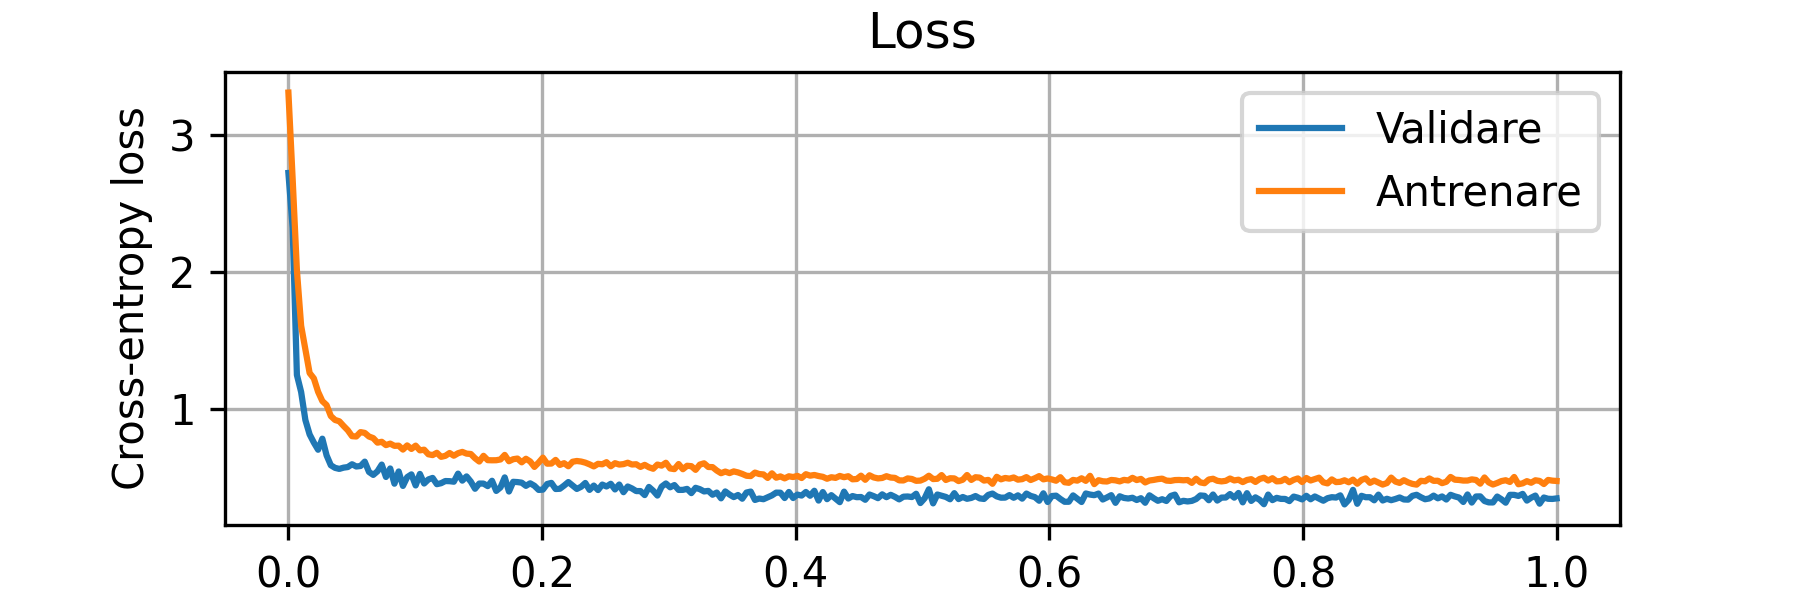
\includegraphics[width=10cm]{images/ocr/loss.png}}
	\end{center}
	\caption{Training results of the CNN network}
	\label{ocr-results}
\end{figure}

\section{Contiguous Training}

As mentioned above, the \textit{EMNIST} dataset we are using only contains alphanumeric characters. We manually added whitespaces, but special characters such as '\code{+}', '\code{-}', '\code{@}' etc. are still not present in the dataset.
\\
To mitigate this issue, we have the following approach:
\begin{enumerate}
	\item When a form is uploaded in order to be parsed, we save an image of the characters we extracted alongside the answer.
	\item If a user edits a parsed form, we assume the user corected a mistake made by the OCR network, and, for each modified character, save in a separate database the now labled image.
	\item Maintainers of the application can train the network again, taking into account the newly created dataset.
\end{enumerate}

This approach is ideal, as SmartForms generates a dataset from the same universe as the characters it has to parse, and over time less and less mistakes are made due to the larger and larger dataset.

% Aici vorbesc despre fastapi, si cum il folosesc in aplicatie
\chapter{HTTP/S Server and Secure Authentication}

\section{FastAPI Session Middleware}

Our entire API service is written using FastAPI, \textit{a modern, fast (high-performance), web framework for building APIs with Python 3.6+ based on standard Python type hints}\cite{FastAPI}.
\\
FastAPI helps us to validate data received, and automatically generates the OpenAPI\cite{open-api} specification of our service.

In order to authenticate users we use a session middleware. This allows us to use a stateless authentication mechanism, where all of the authentication data is stored within an encrypted cookie on the user's browser.

An API endpoint looks similar to this one, which shows a short message to the users and allows him to login and logout of their account:

\begin{minted}[bgcolor=bg]{python}
@app.get('/')
async def home(request: Request):
    """
    Shows the user its authentication status, and allows him to
    check the documentation, login or logout.
    """
    # retrieve the user's details from the session
    # if the user is not logged in, then the `user` object is None
    user = request.session.get('user')
    email = user['email'] if user is not None else 'Not signed in'

    html = (
        f"<pre>Email: {email}</pre><br>" +
        "<a href='/api/docs'>documentation</a><br>" +
        ("<a href='/api/user/logout'>logout</a>"
            if user is not None else
            "<a href='/api/user/login/'>login</a>")
    )
    return HTMLResponse(html)
\end{minted}

By default, \textit{FastAPI} only handles requests over \textit{HTTP}, but one can use a web-server such as \textit{Nginx}\cite{nginx} to act as a HTTP endpoint and proxy for our service.

The setup currently running on the \url{https://smartforms.ml} website, made as part of ???\cite{felix} is the following:
\begin{itemize}
	\item \textit{SmartForms API} is running on \code{0.0.0.0:5000}.
	\item \textit{Nginx} is binded to \code{0.0.0.0:443} and \code{0.0.0.0:80}, and proxies any requests made to the \code{/api/} route to \code{localhost:5000}, which is the API server. 
\end{itemize}

Please note that both services are binded to the meta-address \code{0.0.0.0}, which makes them accessible over all networking interfaces. This means in particular that the API server is exposed to the interned by accessing the \url{http://smartforms.ml:5000} URL (please note the connection is \code{HTTP} and not \code{HTTPS}). The unsecure connection might seem problematic, but, as it can only be used by users forging requests, this is not a security issue, and can be stopped by binding the API service to \code{localhost} instead. Figure \ref{smartformsml-diagram} shows a diagram of the entire service.


\begin{figure}[!h]
	\centering
	\fbox{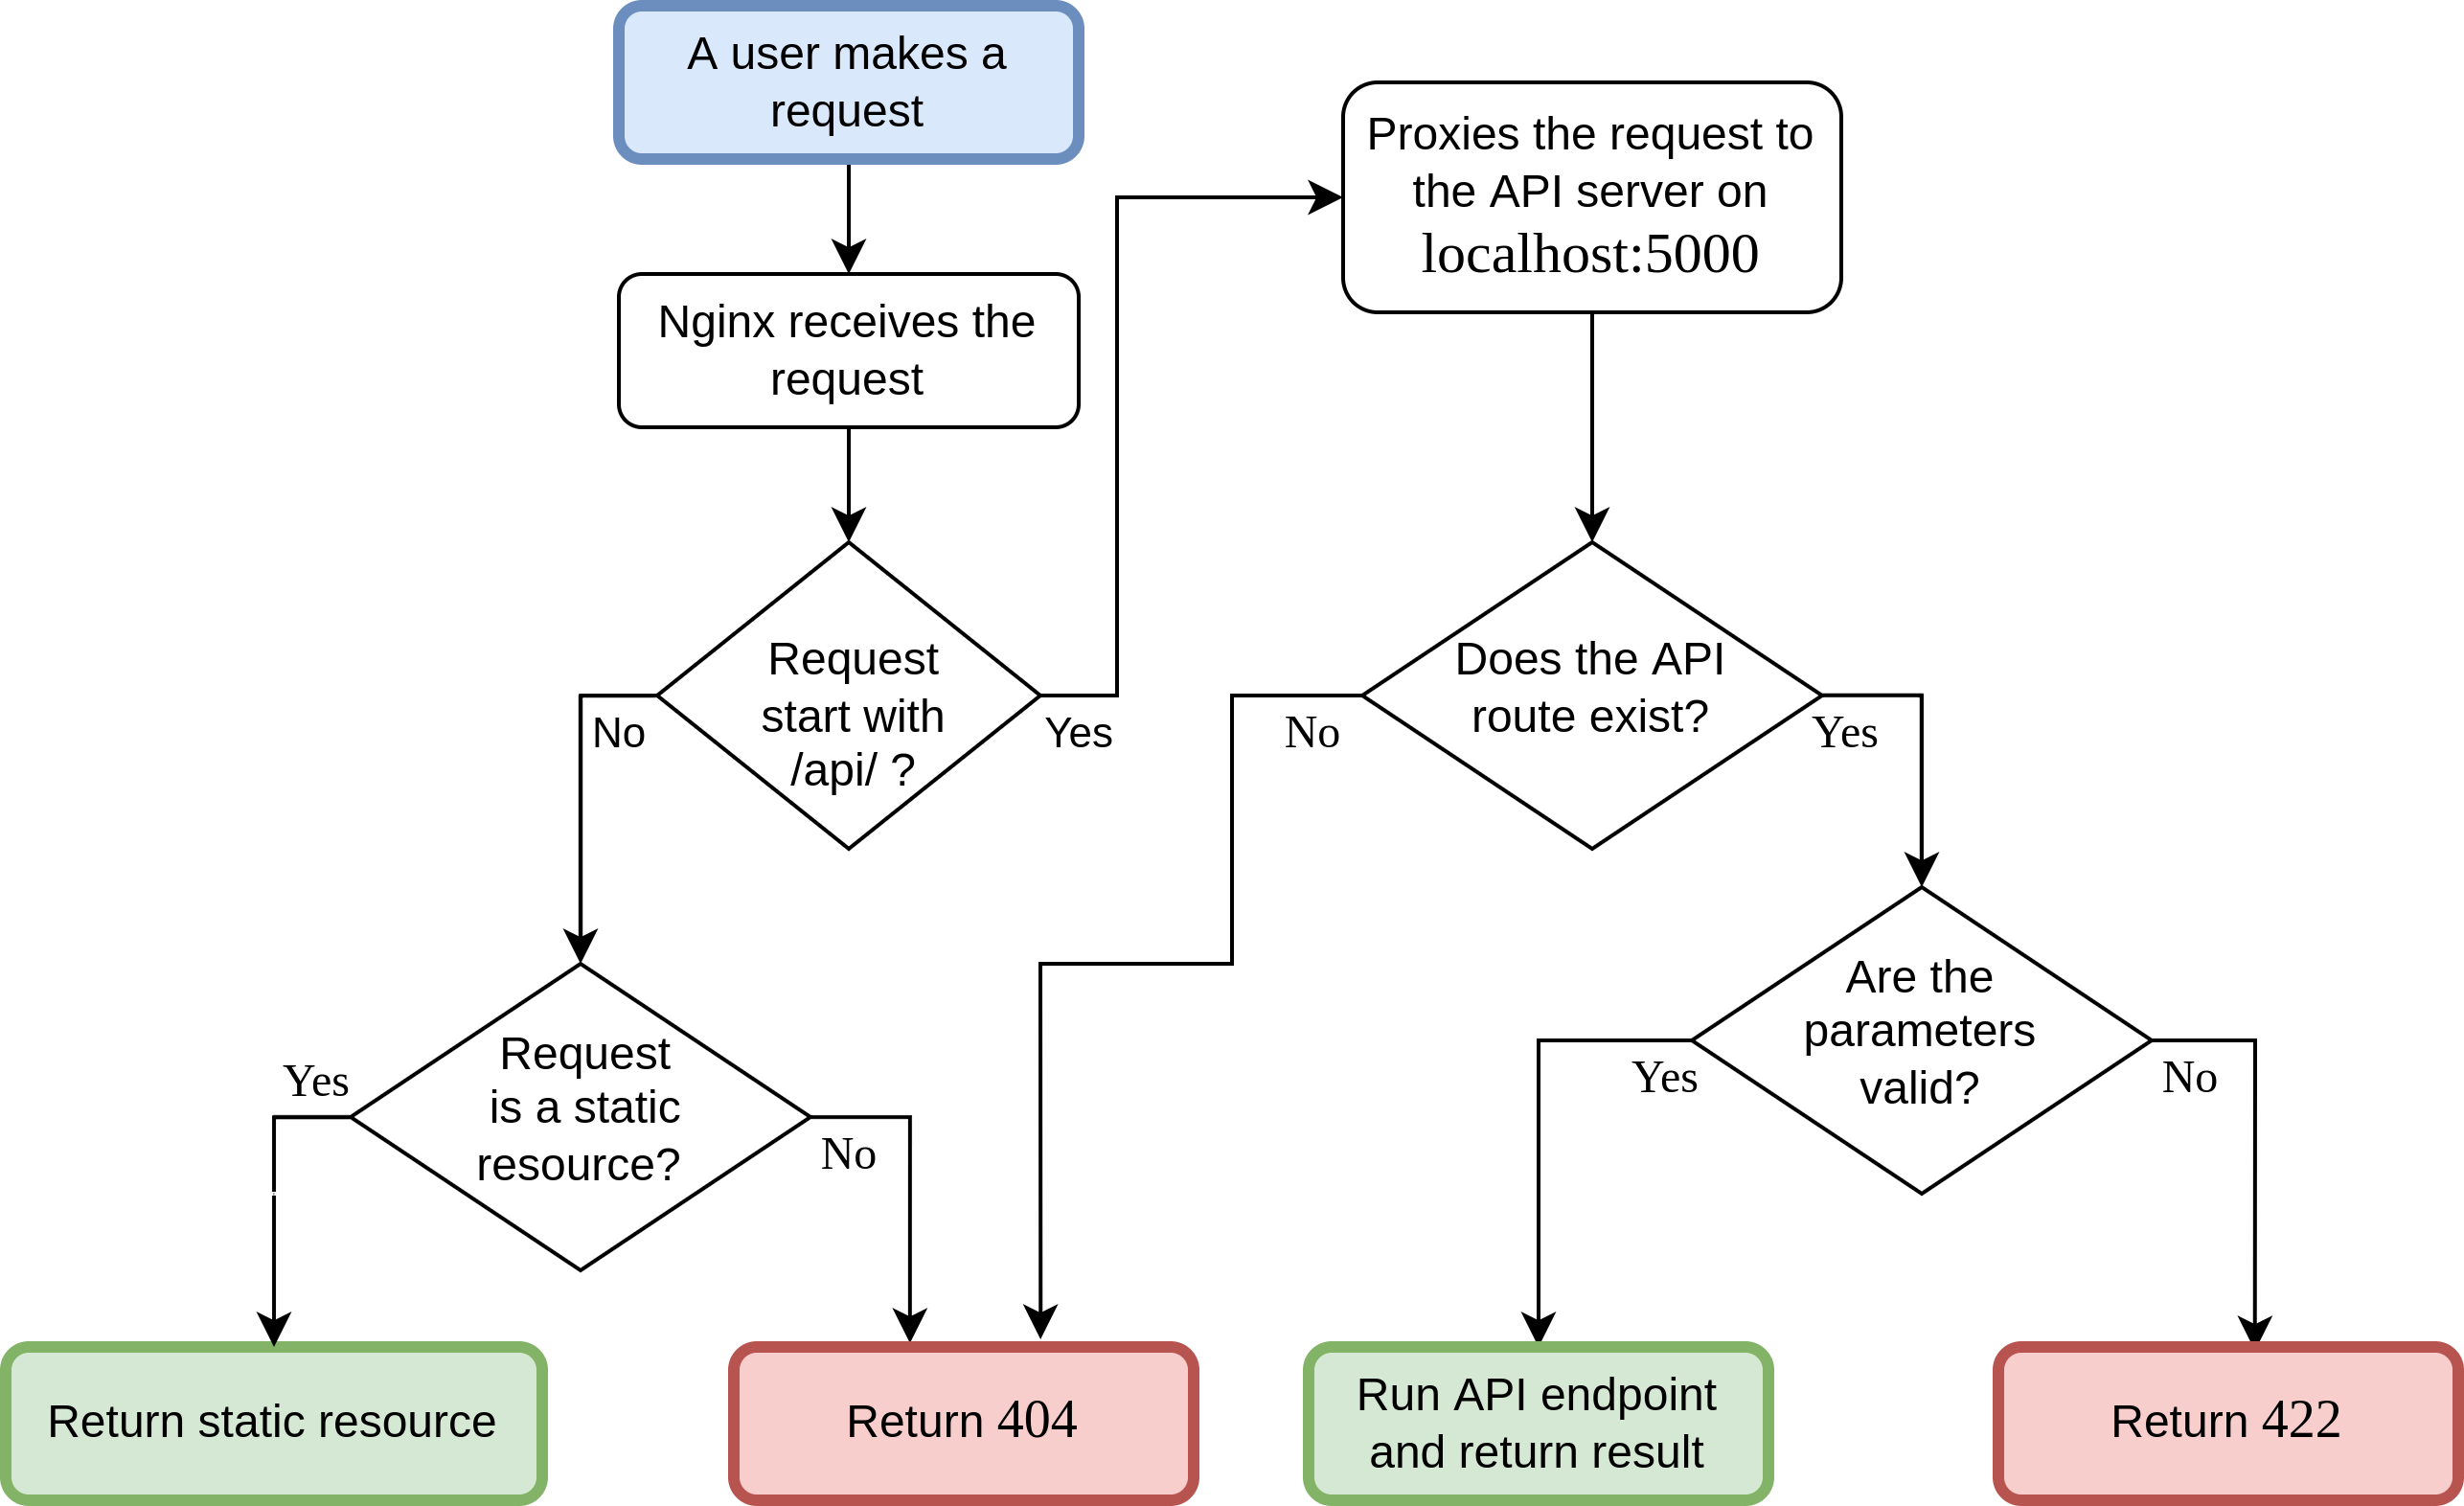
\includegraphics[width=13cm]{images/diagrams/smartformsmlsetup.png}}
	\caption{\url{https://smartforms.ml/} service diagram}
	\label{smartformsml-diagram}
\end{figure}


\section{Oauth2 Authentication Framework}

As SmartForms is a small application, requiring users to create an account with a username and password is tidious. We decided to use the \textit{OAuth v2.0}\cite{oauth2} (\textbf{O}pen \textbf{Auth}entication) protocol, which allows users to login using a $3^\textrm{rd}$ pary account, such as a Facebook, Google or Microsoft account.

Due to the difficulty to open register SmartForms as an OAuth service on most platforms (we need to show a proof we own a domain, ask for human verification, add a credit card etc) we have only registered our application on with Google Cloud.

This means that in its current state SmartForms only allows for authentication using a Google account, but adding additional services only requires a few lines of code besides registering SmartForms on said services.


% Vorbesc despre cum a functionat git, CI/CD, sincronizare cu Felix
\chapter{Tests, Source Control and CI/CD}

\section{Testing}

To ensure a high stability of the application and help speed up the development process we decided to use the \textit{TDD} (\textbf{T}est \textbf{D}riven \textbf{D}evelopment) approach: each API endpoint and all features of SmartForms are thoroughly tested by unit tests.

We also have integration tests, running the application end-to-end (generating forms, creating, modifying and uploading answers).

The only components of the application which are not tested by unit tests are:
\begin{itemize}
	\item The CNN training module, which is technically part of the software, but is only runned manually or if the network model is not found, which only happens due to human intervention.
	\item The \code{user} router, which can hardly be tested as it performs requests to Google Cloud. Testing the endpoints would require creating a test account on Google, extracting its authentication cookies, and manually forging a request to authenticate it on SmartForms, which is almost impossible and strongly forbidden by the Google terms\&conditions. 
\end{itemize}

The total coverage of our unit tests is of $85\%$, which might seem low, but most of the untested lines of code live either in the two modules mentioned above, or hard to reach sections which were manually tested during development.

\section{Git}

We are using Git\cite{Git} as a source control software, and use the Github platform as a remote. The entire project can be viewed online at \url{https://github.com/TeamUnibuc/SmartForms/}, where the entire history of the project (commits, pull requests and issues) is public. Please note that the repository contains SmartForms API as well as the SmartForms client, which is not part of our project, due to their tight connection.

The repository (backend and frontend combined) has over $300$ PRs and commits on the main branch, $35$ active branches and a total of $36.000$ added and $14.000$ deleted lines of code thoughout its history. 


\section{CI/CD}

The \textit{SmartForms} repository is set-up using \textbf{C}ontiguous \textbf{I}ntegration and \textbf{C}ontiguous \textbf{D}eployment pipelines. They are used in the following scenario:
\begin{enumerate}
	\item A developer wants to add a new feature to the project. He branches off from the master branch and implements the feature on the newly created branch.
	\item Once the feature is finished, the developer makes a \textit{pull request} -- also called \textit{merge request}, asking for his/her squashed commits to be applied to the master branch (instead of applying the squashed commits, a rebase or a simple merge are also possible, but less common).
	\item The \textbf{CI} pipeline kicks in, automatically running a series of checks and tests.
	\item If the tests succeed, and the branch is merged, the \textbf{CD} pipeline starts, pushing the entire code from the master branch to production.
\end{enumerate}

The contiguous deployment pipeline is written and mentained by ????\cite{felix}, but the integration one is written by us:

\begin{minted}[bgcolor=bg]{yaml}
# .github/workflows/backend.yml

name: Run Backend Unittests

on:
    push:
        branches: [ main ]
    pull_request:
        branches: [ main ]
        types: [ opened, synchronize ]
jobs:
    build:
        # avoids running AFTER a merged PR
        if: "!contains(github.event.head_commit.message,
                                         'Merge pull request #')"
        runs-on: ubuntu-latest

        steps:
            - uses: actions/checkout@v2
            - name: Set up Python 3.10
              uses: actions/setup-python@v2
              with:
                  python-version: "3.10"
            - name: Install dependencies
              run: |
                sudo apt-get install -y libzbar0 poppler-utils
                python -m pip install --upgrade pip
                pip install flake8 pytest
                pip install -r backend/requirements.txt
            - name: Lint with flake8
                ...
            - name: Test with unittest
              env:
                MONGO_USER: ${{ secrets.MONGO_USER }} 
                MONGO_PASSWORD: ${{ secrets.MONGO_PASSWORD }}
                ...
              run: |
                (cd backend/sources/tests/ && python -m unittest)
\end{minted}

The code shown above does:
\begin{enumerate}
	\item Check if the code being tested is part of a PR, and stops if not. 
	\item Install required packages on the machine -- both \textit{Debian} packages with \code{apt}, and \textit{Python} packages with \code{pip}.
	\item Sintactially check the code with \code{flake8}, a \textit{Python} linter.
	\item Run the backend unit and integration tests.
\end{enumerate}

% vorbesc de ce poate fi adaugat in plus
\chapter{Conclusion and Future Work}

\section{Possible Enhancements}

The software presented in this project is a MVP of a modern online forms and surveys generation and parsing tool. There however many areas in which the project can be extended.

\subsection{User Roles}

The \textit{SmartForms} API does not currently have any support for user roles, such as moderators or administrators. This is purely by design, as we did not consider it essential for our product -- as we use MongoDB, any modifications to users, forms or answers can easily be made directly from the database.

Adding user roles would however make the application more attractive to large corporations, where each employee has a specific set of attributions and authorizations.

\subsection{Stateless PDF Forms}

An important improvement we could have made, but decided against due to the centralized design of our application, is to save any form-related information directly on QR codes.

Currently, QR codes store the ID of the form they are printed onto, which is then used to retrieve from the database details about the form, in order to parse it. We can shortcircuit and completly eliminate the need for a database (in the matching process) by storing on the QR codes all of the details of the form.

While the amount of information to store might seem excessive, people already managed to fit an entire GUI game on single QR code\cite{game-qr-code}, which offers up to a few kilobytes of storage, depending on the error-correction level.

\subsection{Multithreading}

An important improvement speed-wise would be introducing multi-threading to our parsing pipeline. While the OCR model is hard to be ran in paralel as it might be running on the GPU, preprocessing such as QR code extraction, adaptive thresholding, features extraction\&matching and even dataloaders for the CNN could be ran in paralel, to fully utilize more than one CPU core. 


\subsection{Offline Login System}

\textit{SmartForms} relies on online $3^\textrm{rd}$ party authentication. While authentication checks can be disabled altogether by editing the '\code{.env}' file, being able to manage the access to forms and answers could be useful, even in offline scenarios.

\subsection{Additional Input Formats}

Another addition to \textit{SmartForms} could be the introduction of additional input formats, such as a large square for a signature, or a more advanced question format, mimicking questionaires of the form ``When I go to school I have to walk ..... km and it takes ..... minutes", in which text and answer boxes are mixed.

\section{Conclusions}

\textit{SmartForms} was an idea that came up with while helping a front desk worker transcribe a form I had just filled into his computer, one of the situations \textit{SmartFroms} solves. The API, form generation, and form parsing modules went through multiple iterations of approaches and technologies used before ending up in the current state, which we hope is the perfect balance of simplicity and usability, as \textit{SmartForms API} aims to offer a simple yet effective interface for managing questionaires and surverys.

The hardest part of the project has been by far the form parsing pipeline, due to many reasons, such as:
\begin{itemize}
	\item As data is comming from users, we cannot assume that the file format is recognized, files are not corrupted, images contain a valid form, the form exists etc.
	\item The process uses real-world images, which cannot be accuratly created digitally, which translated into a lot of printed forms, scans with various settings, pictures under different lighting conditions and angles and so forth.
	\item We had to make the existing dataset used for training the OCR CNN mimic our data. To check the real accuracy of the network, we had to also create a small verification dataset from scratch.
\end{itemize}

We have not talked too much about the client of \textit{SmartForms}, as it is not part of this project, but the two components (\textit{SmartForms API} and the \textit{SmartForms} client) work perfectly together, making the inner workings of the API completly transparent to the user.


While the software can still be improved, we believe it is already fit for being used by people or institutions for which \textit{SmartForms} presents attractive features, which in our opinion, makes the entire project an overall success.

\begin{thebibliography}{99}	

\bibitem{wicker1999reed}
S.~B.~Wicker, V.~K.~Bhargava,
\emph{Reed-Solomon codes and their applications},
John Wiley \& Sons, 1999.

\bibitem{masinter1998rfc2388}
L.~Masinter, 
\emph{RFC2388: Returning Values from Forms: multipart/form-data},
RFC Editor, 1998.

\bibitem{opencv-color-convention}
\emph{OpenCV: Color Conversions}, n.d., accessed 29 May 2022,  https://docs.opencv.org/3.4/de/d25/imgproc\_color\_conversions.html.

\bibitem{opencv-image-threshold}
\emph{OpenCV: Image Thresholding}, n.d., accessed 29 May 2022,
https://docs.opencv.org/4.x/d7/d4d/tutorial\_py\_thresholding.html

\bibitem{checker-illusion}
E.~H.~Adelson, Pbroks13, \emph{checker shadow illusion}, accessed 29 May 2022, https://commons.wikimedia.org/w/index.php?curid=75000950.

\bibitem{rublee2011orb}
E.~Rublee, V.~Rabaud, K.~Konolige, G.~Bradski,
\emph{ORB: An efficient alternative to SIFT or SURF},
	2011 International conference on computer vision, IEEE (2011),
	2564--2571.

\bibitem{HOG}
N.~Dalal, B.~Triggs,
\emph{Histograms of oriented gradients for human detection},
2005 IEEE computer society conference on computer vision and pattern recognition, IEEE (2005), Vol. 1, 886--893.

\bibitem{CNN}
K.~O'Shea, R.~Nash,
\emph{An introduction to convolutional neural networks}, arXiv preprint
arXiv:1511.08458, 2015.

\bibitem{pytorch}
\emph{Pytorch documentation}, n.d., accessed 30 May 2022,
https://pytorch.org/docs/stable/index.html.

\bibitem{resnet}
K.~He, X.~Zhang, S.~Ren, J.~Sun, 2016,
\emph{Deep residual learning for image recognition},
2016 IEEE conference on computer vision and pattern recognition, IEEE (2016), 770--778.

\bibitem{VGG}
K.~Simonyan, A.~Zisserman,
\emph{Very deep convolutional networks for large-scale image recognition}, arXiv preprint arXiv:1409.1556, 2014.

\bibitem{ReLU}
A.F.~Agarap,
\emph{Deep learning using rectified linear units (relu)}, arXiv preprint arXiv:1803.08375, 2018.

\bibitem{emnist}
G.~Cohen, S.~Afshar, J.~Tapson, A.~Schaik,
\emph{EMNIST: an extension of MNIST to handwritten letters}, arXiv preprint arXiv:1702.05373, 2017.

\bibitem{Git}
\emph{Git}, n.d., accessed 30 May 2022,
https://git-scm.com/

\bibitem{FastAPI}
\emph{FastAPI}, n.d., accessed 31 May 2022,
https://fastapi.tiangolo.com/

\bibitem{open-api}
\emph{OpenAPI Specification}, 20 February 2020, accessed 31 May 2022,
https://swagger.io/specification/

\bibitem{authentication-cookies}
J.S.~Murdoch,
\emph{Hardened stateless session cookies},
International Workshop on Security Protocols, Springer (2008),  93--101.

\bibitem{oauth2}
D.~Hardt,
\emph{RFC 6749: The OAuth 2.0 authorization framework}, RFC Editor, 2012.

\bibitem{nginx}
\emph{Nginx}, n.d., accessed 1 June 2022, 
https://nginx.org/en/.

\bibitem{game-qr-code}
MattKC, \emph{Can you fit a whole game into a QR code?}, accessed 2 Jun 2022, https://www.youtube.com/watch?v=ExwqNreocpg, 2020.

\end{thebibliography}
%\printbibliography
%\printbibliography[heading=bibintoc]
\end{document}
